\documentclass[12pt,a4paper,twoside,openright]{report}
\usepackage[pdfborder={0 0 0}]{hyperref}
\usepackage[margin=25mm]{geometry}
\usepackage{standalone}

% my imports
\usepackage{amsfonts}
\usepackage{amssymb}
\usepackage{amsmath}
\usepackage{amsthm}
\usepackage{amscd}
\usepackage{graphicx}
\usepackage{subcaption}
\usepackage{mathpartir}
\usepackage{isabelle}
\usepackage{isabellesym}
\usepackage{comment}
\usepackage[outputdir=output]{minted}
\usepackage{noindentafter}

% bibliography
\usepackage[backend=bibtex, sorting=none]{biblatex}
\bibliography{dissertation}
\bibliography{proposal/proposal}

% minted configuration
\usepackage[gray]{xcolor}
\usepackage{tcolorbox}
\setminted{frame=lines}

\raggedbottom
\sloppy
\clubpenalty1000%
\widowpenalty1000%
\renewcommand{\baselinestretch}{1.1}

\author{Michael Rawson}
\date{2016--17}

% helpful macros
\newcommand{\thetitle}{Verified Metatheory and Type Inference for a Name-Carrying Simply-Typed \(\lambda\)-Calculus}
\newcommand{\ident}[1]{\texttt{#1}}
\newcommand{\infertype}{\mathrm{infer}}
\newcommand{\names}{\mathbb{A}}
\newcommand{\unit}{\mathrm{unit}}
\newcommand{\wrap}[1]{\left(#1\right)}
\newcommand{\swap}{\leftrightarrow}
\newcommand{\dollar}{\mathbin{\textrm{\footnotesize{\textbf{\$}}}}}
\newcommand{\image}{\mathbin{\textrm{\footnotesize{\textbf{\{\$\}}}}}}
\newcommand{\fvs}{\mathrm{fvs}}
\newcommand{\supp}{\mathrm{supp}}
\newtheorem*{definition}{Definition}
\newtheorem{lemma}{Lemma}
\newtheorem{theorem}{Theorem}
\newenvironment{implementation}
 {\bigskip\begin{tcolorbox}[width=\textwidth]\begin{isabellebody}}
 {\end{isabellebody}\end{tcolorbox}\setlength{\leftskip}{0cm}}

% remove indents from paragraphs after some environments
\NoIndentAfterEnv{implementation}
\NoIndentAfterEnv{proof}

\begin{document}
\pagestyle{empty}
\rightline{\LARGE\textbf{Michael Rawson}}
\vspace*{60mm}
\begin{center}
\Huge
\textbf{\thetitle}\\[5mm]
Computer Science Tripos -- Part II\\[5mm]
Robinson College\\[5mm]
\today
\end{center}

%proforma
\pagestyle{plain}
\chapter*{Proforma}
{\large
\begin{tabular}{p{0.3\textwidth}p{0.7\textwidth}}
Name:              & \bf Michael Rawson\\
College:           & \bf Robinson College\\
Project Title:     & \bf \thetitle\\
Examination:       & \bf Computer Science Tripos -- Part II, July 2017\\
Word Count:        & 11,976\footnotemark[1]\\
Project Originator:& Dr. Dominic Mulligan\\
Supervisors:       & Dr. Dominic Mulligan and Dr. Victor Gomes\\
\end{tabular}
}
\footnotetext[1]{As computed by \emph{texcount}}
\stepcounter{footnote}

\section*{Original Aims of the Project}
I aim to create a mechanisation in Isabelle of the simply-typed \(\lambda\)-calculus, together with a verified algorithm for type inference.
Emphasis is placed on the treatment of binders in the calculus and the approach taken with representing \(\alpha\)-equivalence.

\section*{Work Completed}
This project meets all proposed success criteria, and adds two extensions.
I have implemented the calculus, encoded the \(\alpha\)-equivalence equivalence relation, and specified typing rules and a type inference algorithm for the calculus.
A number of correctness proofs accompany this implementation.
Further to this, I implemented extensions, one to add unit and pair values and corresponding types to the implementation, and one to show the confluence property of the calculus.

\section*{Special Difficulties}
None.

\newpage
\section*{Declaration}
I, Michael Rawson of Robinson College, being a candidate for Part II of the Computer Science Tripos, hereby declare that this dissertation and the work described in it are my own work, unaided except as may be specified below, and that the dissertation does not contain material that has already been used to any substantial extent for a comparable purpose.

\bigskip
\leftline{Signed }
\medskip
\leftline{Date }
\tableofcontents

\newpage
\section*{Acknowledgements}
I wish to acknowledge the efforts of my supervisors in guiding me in this project.
Both offered advice when I needed it, and let me get on when I didn't --- an unusual and invaluable skill!

\pagestyle{headings}

\chapter{Introduction}
This dissertation describes my part II project for the Computer Science Tripos, entitled \emph{Verified Metatheory and Type Inference for a Name-Carrying Simply-Typed \(\lambda\)-Calculus}.
The project consists of a series of machine-checked proofs about a typed \(\lambda\)-calculus, a type inference algorithm for the calculus, and a checked proof of correctness of the algorithm.

\section{Motivation}
After stating my interest in typed \(\lambda\)-calculi and computerised implementations thereof, my supervisor suggested that I implement a calculus, then prove it correct.
Proofs about systems involving names are famously fiddly, so a proof-checker would be used to ensure the proofs asserting the implementation correct were themselves sound.

Therefore, the project had several principle motivations:
\begin{itemize}
\item
produce a high-quality implementation of a typed calculus, encoded in a proof assistant
\item
ensure the implementation is correct --- informal pen-and-paper arguments are prone to error, so I had to provide formal, verified proofs in the assistant
\item
extract working code that is proven to be correct
\end{itemize}
\section{Related Computer Science}
The project draws on a wide-variety of areas in Computer Science: type theory, logic, formal verification and even HCI.

By verifying a \emph{typed} calculus, the project required some theory about types, including proving properties such as the preservation of types under \(\beta\)-reduction.
Verification itself requires some knowledge (and precise application) of logic, despite the best efforts of the proof-checking software.
Additionally, the approaches taken with informal proof versus those with verified proof remain extremely different: while largely the informal proof's structure remains in a formal proof, fiddly details require some knowledge of common verification techniques and some specialist software knowledge.

Finally, one aim of the project was to be easy to use and modify by others.
The exact internal presentation of the calculus used in the verification does not usually matter, but if external users unfamiliar with the implementation details are to use it effectively, the presentation must include several niceties that might not otherwise be used.
Picking the presentation of the calculus that minimises the effort required to use it required some thought about usability and interactions users might have.

\section{Previous Work}
Not sure what to put in this section. Lots of previous work!

\chapter{Preparation}
\label{chap:preparation}
After identifying the main goals, these coarse requirements are refined to be precise about objectives, and to drive development.
This results in a set of \emph{requirements} that can be analysed to predict problems and measure success.
Once any problems are resolved, work can begin on implementation.
Some mathematics is required to increase precision, and can be used to direct refinement of requirements.
In this chapter I discuss the theory required to begin formalisation, briefly introduce Isabelle, and produce a list of requirements.

\section{\(\lambda\)-Calculus}
\label{sec:lambda-intro}
The \(\lambda\)-calculus~\cite{lambda-overview} is a system of computation, represented by operations on \emph{terms}.
\begin{definition}
Terms \(M\) are inductively defined:
\begin{enumerate}
\item
A variable, \(x\), is always a term.
These may be sub-categorised to be \emph{bound} if some \emph{binder} in an expression binds them, or \emph{free}, if there is no such binder.
\item
If \(M\) is a term, abstractions \(\lambda x.M\) are also terms.
This intuitively represents an anonymous function returning \(M(x)\)), and \emph{binds} \(x\) in \(M\).
\item
If \(M\) and \(N\) are terms, applying \(M\) to \(N\) is also a term, \(\wrap{M\ N}\).
\end{enumerate}
\end{definition}

\noindent
Terms can be represented with an algebraic datatype.
For instance, in Standard ML:
\begin{minted}{SML}
datatype 'a trm =
    Var of 'a
  | Fn  of ('a * 'a trm)
  | App of ('a trm * 'a trm)
\end{minted}

Computation here is performed by \(\beta\)-reduction: terms \emph{reduce} to another term according to a series of rules, and hence computation occurs by sequential reductions.

\begin{definition}
\(M \to_\beta M'\) when one of the following holds:
\begin{enumerate}
\item
If left or right subterms of an application reduce, then the application also reduces: if \(M \to_\beta M'\), then \(\wrap{M\ N} \to_\beta \wrap{M'\ N}\).
\item
If \(M \to_\beta M'\), then \(\lambda x.M\) becomes \(\lambda x.M'\).
\item
If a term is of the form \(\wrap{\wrap{\lambda x.M}\ N}\), then it is a \(\beta\)-redex, and reduces to
\[
M[x := N]
\]
(\emph{viz.} \(M\) with occurrences of \(x\) substituted in a capture-avoiding fashion for \(N\)).
\end{enumerate}
\end{definition}

The order in which reduction steps occur in a computation is important for many applications of the \(\lambda\)-calculus, but I did not use this property in my dissertation.
Substitution, used informally above, is defined recursively.

\begin{definition}
Suppose \(N\) is substituted for \(x\) in \(M\), and \(y\) is any name that is not \(x\).
Then the result, \(M[x := N]\), is
\[
M[x := N] =
\begin{cases}
N & M = x\\
M & M = y\\
M & M = \lambda x. M'\\
\lambda y. \wrap{M'[x := N]} & M = \lambda y. M'\\
\wrap{M_1[x := N]\  M_2[x := N]} & M = \wrap{M_1\ M_2}\\
\end{cases}
\]
\end{definition}

\(\beta\)-reduction has \emph{confluence} property.
Confluence states that if \(A\) reduces in many steps to \(B\), and similarly on another path to \(C\), there is a \(D\) such that \(B\) and \(C\) reduce to \(D\), asserting that the order of reductions does not affect the final result.
There are terms that cannot be further reduced, like \(x\), \(\lambda y.y\), or \(\wrap{f\ x}\).
These terms are considered to be values, or \emph{in normal form}.

\begin{definition}
Variables \(x\) are in normal form.
Applications are in normal form if they are not a \(\beta\)-redex and both subterms are themselves in normal form.
Binders are in normal form if their bound subterm is in normal form.
\end{definition}

\section{Simple types}
\label{sec:type-intro}
Untyped calculi have disadvantages.
No types mean that unexpected constructions can occur, such as applying a non-function, which a type system generally prevents.
``Programs'' in the calculus may also fail to terminate: a sequence of reductions may not necessarily finish.
Consider

\[
\Omega = \wrap{\lambda x. \wrap{x\ x}}\ \wrap{\lambda x. \wrap{x\ x}}
\]

Then the only possible reduction for \(\Omega\) produces \(\Omega\), which may not terminate.
The untyped calculus can be extended to include a type system while maintaining an approach to names: a \emph{type} is simply added to each binder, so \(\lambda x.M\) becomes \(\lambda (x:T).M\), for an arbitrary \(T\).
Note that I use this, the Church style of typing, exclusively in my project.

\begin{definition}
Simple types \(\tau\) are either
\begin{enumerate}
\item
A base type, say \(\iota\).
\item
An arrow type \(\tau_1 \to \tau_2\) from one type to another.
\end{enumerate}
\end{definition}

Adding simple types to the binders of the untyped calculus produces the \emph{simply-typed} \(\lambda\)-calculus.
The typing relation \(\Gamma \vdash M : \tau\) is given inductively in Figure \ref{fig:typing}.
\(\Gamma\) here is a typing context: a partial function from variables to types.

\begin{figure}
\begin{mathpar}
\inferrule[var]
 {\Gamma(x) = \tau}
 {\Gamma \vdash x : \tau}

\inferrule[fn]
 {\Gamma\{x \mapsto \tau\} \vdash M : \sigma}
 {\Gamma \vdash \lambda (x : \tau). M : \tau \to \sigma}

\inferrule[app]
 {\Gamma \vdash M : \tau \to \sigma \\ \Gamma \vdash N : \tau}
 {\Gamma \vdash \wrap{M\ N} : \sigma}
\end{mathpar}
\caption{typing rules for the simply-typed calculus}
\label{fig:typing}
\end{figure}

I show several correctness properties that are not possible in an untyped calculus: progress, type preservation (subject reduction), and safety.
These capture semantics of Milner's~\cite{milner} maxim ``well-typed programs do not go wrong''.

\begin{definition}
The progress property asserts if \(\Gamma \vdash M : \tau\), \(M\) is either in normal form or can be reduced further.
\end{definition}

\begin{definition}
The preservation property holds if, assuming \(\Gamma \vdash M : \tau\) and \(M\) reduces to \(M'\), \(\Gamma \vdash M' : \tau\).
\end{definition}

Generally these are desirable properties: expressions should not ``get stuck'' computing non-values, or change type mid-reduction.

\begin{definition}
A language has the safety property if, when reducing a well-typed term \(M\) by a number of steps resulting in \(M'\), \(M'\) is either in normal form, or can be reduced further.
\end{definition}

This property is the main goal of verification: it shows that if a term is well-typed, there is no scenario in which reduction fails --- the term reduces, or computation has finished.

\begin{center}
\rule{.3\textwidth}{.5pt}
\end{center}

Type inference is the process of producing a type \(\tau\) for \(M\) such that \(\Gamma \vdash M : \tau\).
One advantage of the simply-typed calculus is that type inference is decidable, and straightforward, with no unification steps (in the Church style) or complexity that more advanced typing systems encounter.
The type inference algorithm \(\infertype(\Gamma, M)\) can be described by
\[
\infertype\wrap{\Gamma, M} =
\begin{cases}
\Gamma(x) & M = x\\
\tau \to \infertype\wrap{\Gamma\{x \mapsto \tau\}, N} & M = \lambda (x : \tau). N\\
\mathrm{apply}\wrap{\infertype\wrap{\Gamma, A}, \infertype\wrap{\Gamma, B}} & M = \wrap{A\ B}
\end{cases}
\]
where \(\mathrm{apply}\wrap{\tau \to \sigma, \tau}\) produces \(\sigma\).
All other input is undefined.
I use an option type to propagate errors upwards, which the above omits for simplicity.
Type inference can be shown correct with respect to a type system if it exclusively infers correct types (\emph{soundness}), and infers all possible correct types (\emph{completeness}).
With these properties, the typing rules and the inference algorithm are equivalent.

\section{The problem of \(\alpha\)-equivalence}
\label{sec:alpha-equivalence}
This representation, with names and binders, is insufficient.
It is convenient to reason that e.g. \(\lambda x.x\) and \(\lambda y.y\) are equal: they produce identical results on all inputs.
However, they differ structurally: \(x\) is not the same as \(y\).
This reasoning is called \emph{\(\alpha\)-equivalence}.

\begin{definition}
The \(\alpha\)-equivalence relation \(\equiv_\alpha\) is the least congruence on terms such that
\[
\lambda x.M \equiv_\alpha \lambda y.M'
\]
where y does not occur free in \(M\), and \(M'\) is \(M\) with \(x\) substituted for \(y\) (avoiding captures).
\end{definition}

Such an equivalence could be assumed whenever required.
Nonetheless, it is cumbersome to carry such an assumption, and proof assistants often reason better about equality than equivalence relations, as automation tools are tuned for equality.
This problem can be solved using \emph{quotient types}~\cite{quotient}.

\begin{definition}
A quotient type \(Q\) is a base type \(R\), an equivalence relation \(\sim\) on \(R\), and functions \(\mathrm{Abs} : R \to Q\) and \(\mathrm{Rep} : Q \to R\).
Items \(q_1 : Q\) and \(q_2 : Q\) are equal iff \(Rep\ q_1 \sim Rep\ q_2\).
\end{definition}

I now define a quotient type for \(\lambda\)-terms modulo \(\alpha\)-equivalence by encoding a datatype for pre-terms without equivalence as before, then the new type is a quotient over \(\alpha\)-equivalence.
While we now use equality directly, this equivalence relation is awkward to use.
There are alternative ways of handling names, the most prominent de Bruijn indices~\cite{deBruijn}, Higher-Order Abstract Syntax~\cite{HOAS} (HOAS), and nominal techniques~\cite{nominal}.
Ideally, these would allow the ``Barendregt convention'' for reasoning about names: for any term, assume that the bound variables are distinct, and fresh for a given set~\cite{lambda-overview}.
This simplifies proofs about name-carrying syntax, and is useful in informal reasoning about \(\lambda\)-calculus.

De Bruijn indices remove names altogether, and instead use natural numbers for bound variables to refer to the number of other binders between the variable and the respective binder.
\[
\lambda x. \lambda y. x
\]
becomes
\[
\lambda.\lambda. 1
\]
using de Bruijn indices.
\(\alpha\)-equivalence is now equality, as all bound names have been removed.
The downside is that using this representation for argument is unintuitive, using numbers rather than names.
There are variations on these indices, including de Bruijn levels (counting binders from the start, not relative to the variable --- the constant function becomes \(\lambda.\lambda. 0\)), and conventions separating free and bound variables~\cite{i-am-a-free-variable} syntactically, but the disadvantage stands: reasoning is complicated by arithmetic.

HOAS uses the host's (in this case Isabelle) own implementation of names to handle binding.
The datatype presented earlier would then be

\begin{minted}{SML}
datatype trm =
    Fn  of (trm -> trm)
  | App of (trm * trm)
\end{minted}

\(\lambda x.\lambda y.x\) would be represented as \mintinline{SML}{Fn (fn x => Fn (fn y => x))}.
While this implementation avoids many issues of other approaches, it is not possible to show certain properties with this representation~\cite{HOAS}.
Manipulating terms also becomes difficult, as binders have to be applied to access their terms.
Additionally, this representation is negative, so cannot be represented in many proof assistants, which require strictly-positive datatypes to avoid inconsistencies~\cite{inductive-types}.
Theoretical issues arise from the ability to place arbitrary host terms under binders, some of which may non-terms, so the representation is too permissive and allows ``junk terms''.

Parametric HOAS~\cite{PHOAS} removes some problems by re-introducing explicit variables, and parameterising binders over a set of names.
The approach reduces the effect of junk terms (since only terms depending on names are expressible), and the datatype is now strictly-positive:

\begin{minted}{SML}
datatype 'var trm =
    Var of 'var
  | Fn of ('var -> 'var trm)
  | App of ('var trm * 'var trm)
\end{minted}

Finally, the ideas of ``nominal techniques''~\cite{nominal} introduced by Gabbay and Pitts are a new approach, which retain the explicit representation of names, as in the na\"ive version.
The technique uses a definition of \(\alpha\)-equivalence based on \emph{permuting} names in a given expression.
I chose this approach, as it allowed a natural representation of the calculus, without compromising usability or theoretical properties, but allowing concise arguments.

Several further techniques exist, including recent research into viewing \(\lambda\)-terms as maps of occurrences of variables in a tree~\cite{term-maps}.
The area of binders is still active, with new approaches in continuous development.

\section{Nominal techniques}
\label{sec:nominal-intro}
I use the following simplified presentation of the nominal idea of \(\alpha\)-equivalence in my project, but the theoretical background is more general.
I present the simplified idea first, then an overview of the generality of nominal techniques.

\begin{definition}
A swapping \([x \swap y]\) is a pair of variables \(x\), \(y\).
\end{definition}

These represent changing instances of \(x\) to \(y\) and \(y\) to \(x\) within a structure, leaving other variables unchanged.

\begin{definition}
The effect of a swapping, \([x \swap y] \cdot M\) is defined as
\[
[x \swap y] \cdot M =
\begin{cases}
y & M = x\\
x & M = y\\
z & M = z, z \notin \{x, y\}\\
\lambda ([x \swap y] \cdot z). \wrap{[x \swap y] \cdot N} & M = \lambda z.N\\
\wrap{[x \swap y] \cdot A}\ \wrap{[x \swap y] \cdot B} & M = \wrap{A\ B}
\end{cases}
\]
\end{definition}

An equivalence \(\sim\) can be defined using only this operation, as shown in Figure \ref{fig:nominal} --- the preconditions \(z \# M\) and \(z \# N\) mean that ``\(z\) is \emph{fresh} for \(M\) and \(N\)''.
An element \(x\) is fresh in a set \(S\) iff \(x \notin S\), and a variable \(x\) is fresh for a term \(M\) iff \(x\) is fresh for the free variables of \(M\).

\begin{figure}
\begin{mathpar}
\inferrule[var]
 { }
 {x \sim x}

\inferrule[app]
 {A \sim C \\ B \sim D}
 {\wrap{A\ B} \sim \wrap{C\ D}}

\inferrule[fn]
 {[z \swap x] \cdot M \sim [z \swap y] \cdot N \\ z \# M \\ z \# N}
 {\lambda x.M \sim \lambda y.N}
\end{mathpar}
\caption{an equivalence defined in terms of swappings}
\label{fig:nominal}
\end{figure}
It can be shown~\cite{nominal-binders} that \(\sim\) is equivalent to \(\equiv_\alpha\).
Therefore, my approach to representing terms-modulo-\(\alpha\)-equivalence will be to develop a theory of swappings, then use it to show \(\sim\) is an equivalence relation, and finally produce a new type as a quotient of the concrete type with \(\sim\).
I also need a verified implementation of freshness.

\begin{center}
\rule{.3\textwidth}{.5pt}
\end{center}

\noindent
These definitions suffice for my project.
However, they are a simplification of more general theory, presented briefly here and in more detail elsewhere~\cite{nominal,nominal-talk,gabbay}.

Consider a set \(\names\) of \emph{names}.
Then, there is another set \(\textrm{Perm}(\names)\), which is the set of finite permutations on \(\names\).
This set forms a group: the group operator is composition, and identity is the identity permutation \(\varepsilon\).
Each permutation has an inverse.
Note here that every permutation can be decomposed into a sequence of swappings, permutations which only swap two variables, and hence composition is simply concatenating lists of swappings.

The \emph{action} of a permutation \(\pi\) on a structure \(x \in X\) which contains \(\names\) --- for instance, the set of \(\lambda\)-terms using \(\names\) as variables --- maps \(X\) onto itself, permuting the names in \(x\).

\begin{definition}
The action of \(\pi\) on \(X\), \(\pi \cdot x\), is a function that satisfies \(\pi_1 \cdot \pi_2 \cdot x = \wrap{\pi_1 \circ \pi_2} \cdot x\), and is \(x\) when \(\pi\) is the identity permutation.
\end{definition}

Some set \(\supp(x)\) of names \emph{support} \(x\): if a permutation does not change \(\supp(x)\), the permutation action will not change \(x\).
In the \(\lambda\)-calculus under \(\alpha\)-equivalence, \(\supp(x) = \fvs(x)\), as permuting bound variables will not change the term under \(\alpha\)-equivalence, but changing free variables does change \(x\).

\begin{definition}
A set \(X\) is a nominal set if for each \(x \in X\), \(\supp(x)\) is finite.
\end{definition}

Nominal sets form a category, where objects are nominal sets, and arrows are \emph{equivariant} functions, functions \(f\) that satisfy
\[
f(\pi \cdot x) = \pi \cdot f(x)
\]

\begin{figure}
\[
\begin{CD}
X	@>\pi>>	X\\
@VVfV		@VVfV\\
Y	@>\pi>>	Y
\end{CD}
\]
\caption{A commutative diagram showing the behaviour of an equivariant function.}
\label{fig:equivariant}
\end{figure}

Each nominal set \(X\) yields another nominal set \([\names]X\), whose inhabitants are \emph{name-abstractions} \(\langle a \rangle x\), with an equivalence relation \(\sim\).
\(\langle a \rangle x \sim \langle b \rangle y\) iff there is a new name \(c\), fresh for \(a, b, x, y\) such that \([a \swap c] \cdot x = [b \swap c] \cdot y\).
The permutation action on \([\names]X\) is defined to be such that \(\pi \cdot \wrap{\langle a \rangle x} = \langle \pi \cdot a \rangle\wrap{\pi \cdot x}\).
By using this definition on \(\lambda\)-terms, Gabbay arrives at the definition presented in Figure \ref{fig:nominal}.

\section{Isabelle}
\label{sec:isabelle-intro}
Isabelle~\cite{isabelle} is a logical framework, supporting several object logics (I use Higher-Order Logic, the default), proof methods to remove tedious proof steps, and a human-readable proof language, Isar~\cite{isar-phd}.
Proofs are checked in Isabelle by providing any definitions one wishes to make, then arguing theorems in this context.
Since each step is checked, the theorems must be logically correct with respect to the definitions used.
There are also other features Isabelle provides that I use in my project.

Quotient types are used heavily in my dissertation, for equivalence of permutations, and for \(\alpha\)-equivalence.
Isabelle provides this via the \texttt{quotient\_datatype} command~\cite{isabelle-quotient}, which takes a base type \(R\) and an equivalence relation \(\sim\) and produces a new quotient type \(Q\), \(\mathrm{Abs}\) and \(\mathrm{Rep}\).
It also provides ``lifting'' and ``transfer'' operations to move between the types.
Type classes~\cite{isabelle-typeclasses} are another feature I used, providing a way for types to conform to an interface (for instance, all types that can be ordered might form an ordering typeclass).
I used type classes to implement freshness polymorphically.

A major advantage of Isabelle over others was the straightforward support for quotient types.
Isabelle's rivals Agda and Coq both suffer from ``setoid hell'', in which non-equality equivalence relations must be passed around to reason about propositions involving equivalence.
There is no direct equivalent of \texttt{quotient\_type}, and the theory becomes somewhat involved to implement such a construct~\cite{quotients-hard}.
Isabelle also has excellent tooling and a stable core, and these factors combined made it a good choice for my project.

\section{Requirements analysis and engineering}
\label{sec:requirements}
Moving from coarse requirements to finer ones is now easier, as constraints are imposed by the mathematics.
Implementation can now be broken into the following steps:
\begin{enumerate}
\item
Develop work about freshness and swappings to support later developments.
\item
Define a datatype for representing simple types.
\item
Define \emph{pre-terms}, the raw terms of the calculus.
\item
Define the effect of swappings on pre-terms.
\item
Define the \(\alpha\)-equivalence relation.
\item
Show it is an equivalence relation.
\item
Define a type inference algorithm on pre-terms, show invariance under \(\alpha\)-equivalence.
\item
Produce a quotient type of \emph{terms} from pre-terms under equivalence.
\item
Lift required definitions and lemmas over the quotient.
\item
Prove required theorems by reference to identical results on pre-terms.
\item
Define a typing relation on terms.
\item
Argue safety properties of this typing relation.
\item
Show that the algorithm is sound and complete with respect to the typing relation.
\item
Conclude that the implementation is verified, extract code.
\end{enumerate}

The dependencies between steps are largely sequential, as shown in Figure \ref{fig:requirements-dependencies}, and each step can only be ``complete'', or ``incomplete'', considering the boolean nature of formal verification development.
A waterfall model of development seems appropriate: topological sorting of Figure \ref{fig:requirements-dependencies} would suffice to follow such a model.
However, Isabelle allows admitting propositions as axioms, so to a limited extent each step can follow an iterative model where proofs are progressively made more explicit, with fewer admitted steps.

\begin{figure}
\centering
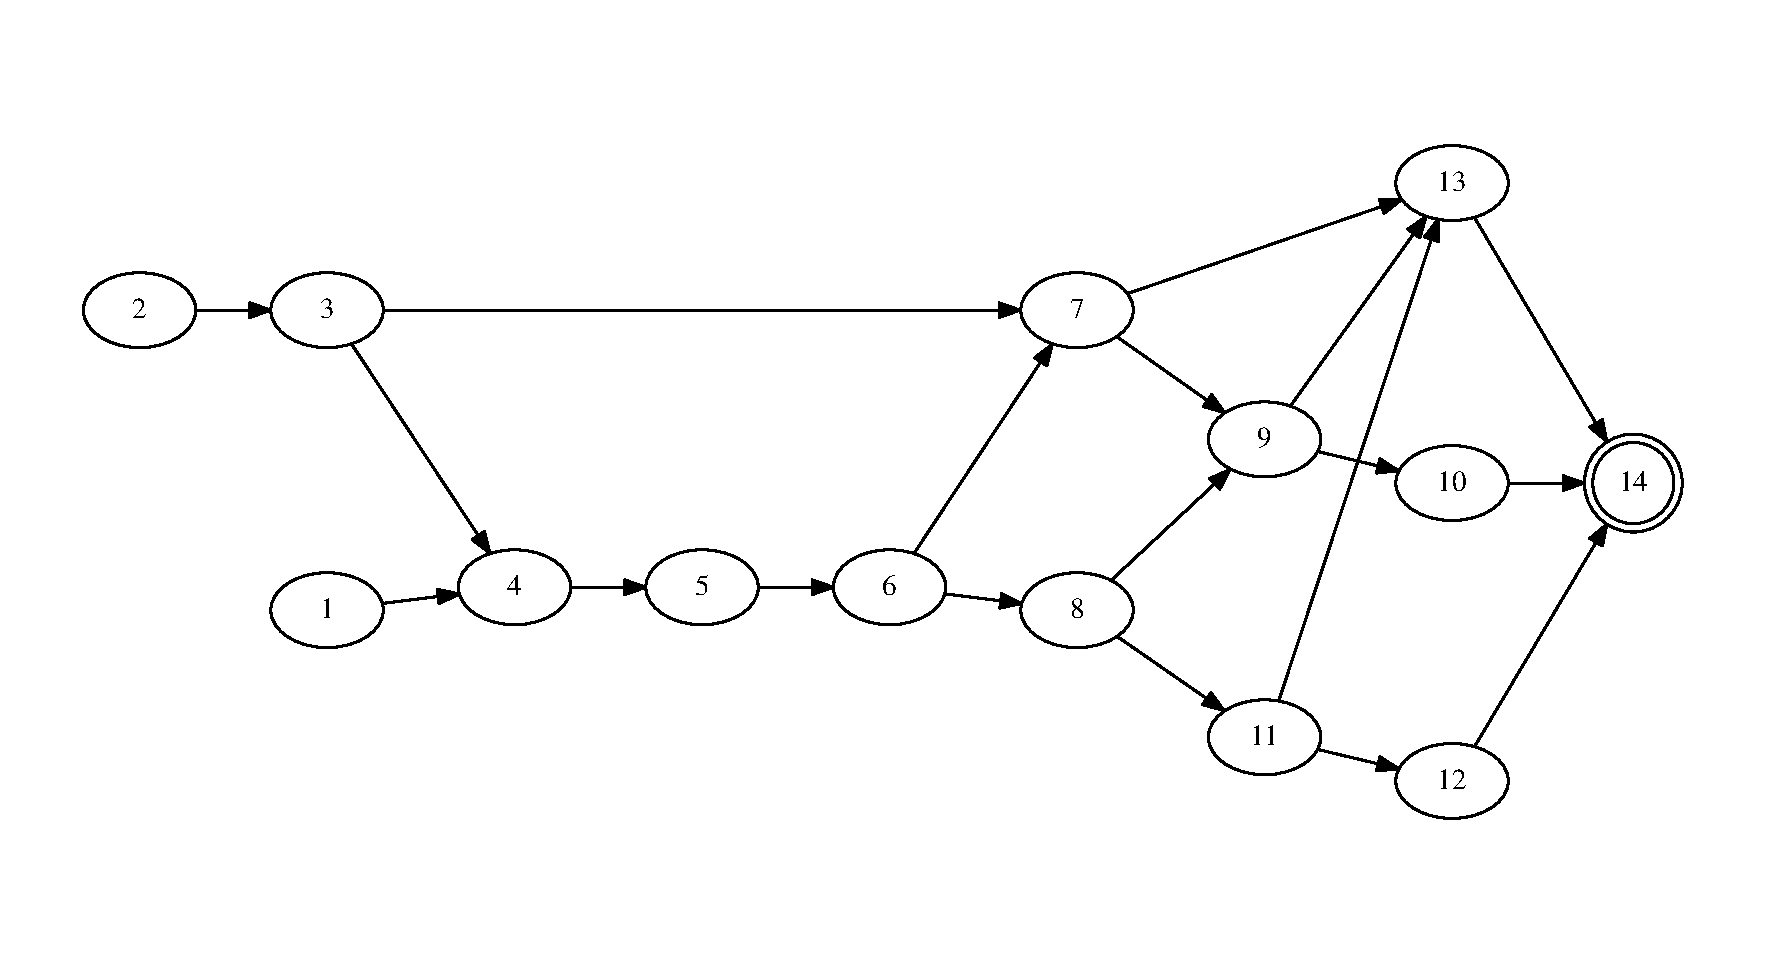
\includegraphics[width=\textwidth]{chapters/preparation/figures/dependencies}
\caption{A directed graph showing which tasks must be completed to begin others. \(A \to B\) shows that \(A\) must be complete before \(B\) may begin.}
\label{fig:requirements-dependencies}
\end{figure}

As far as possible, I followed software engineering good-practice.
All project files were checked into version control (git), and shared (read-only) with supervisors using a well-known hosting website.
Weekly progress meetings were observed to ensure the project did not get off-track.

\section{Starting point}
At the start of the project, I was familiar with the theory required for implementing \(\lambda\)-calculus and type theory.
I was not familiar with approaches to binding described above, or with Isabelle itself.
I am pleased to say I have now learned more about these topics.

\section{Summary}
In this chapter I discussed work that took place before implementation began.
I introduced background theory, covering untyped \(\lambda\)-calculus (\S\ref{sec:lambda-intro}), simple types (\S\ref{sec:type-intro}), \(\alpha\)-equivalence and approaches to this problem (\S\ref{sec:alpha-equivalence}), and introduced nominal techniques (\S\ref{sec:nominal-intro}).
I then described the Isabelle tooling (\S\ref{sec:isabelle-intro}), preparing for practical and theoretical challenges later.
Finally, I decomposed the project into steps (\S\ref{sec:requirements}), and described engineering techniques used to tackle the problem.

\chapter{Implementation}
The work is split into four modules, or what Isabelle calls \emph{theories}.
The first (\emph{Fresh}) deals with fresh names and implementations of freshness, the second (\emph{Permutation}) with a theory of permutations, and the third and fourth (\emph{PreSimplyTyped} and \emph{SimplyTyped}) with \(\lambda\)-terms, before and after the quotient respectively.
All theories develop upon basic theorems shown in Isabelle's standard library, called \emph{Main}.
A dependency graph is shown in figure \ref{fig:dependencies}.

\begin{figure}
\centering
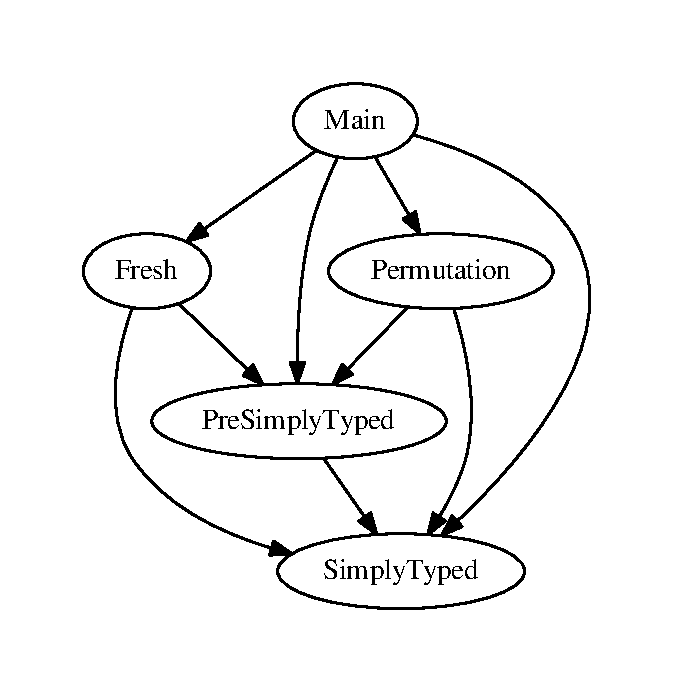
\includegraphics[width=.5\textwidth]{chapters/implementation/figures/dependencies}
\caption{A directed graph showing which of the theories depend on each other. \(A \to B\) shows that \(B\) depends upon results in \(A\).}
\label{fig:dependencies}
\end{figure}

\section{Freshness}
The idea of fresh variables is implemented first, so it can be used later in arguments about fresh names in a given \(\lambda\)-term.
The implementation should take a set (of some type, since we wish to be parametric) and produce an element not in that set.
In order to specify an interface over an arbitrary type, I used Isabelle's typeclass mechanism to make a class (i.e. an interface) for types that can produce a fresh element from a set:

\begin{implementation}
\isacommand{class}\isamarkupfalse%
\ fresh\ =\isanewline
\ \ \isakeyword{fixes}\ fresh{\isacharunderscore}in\ {\isacharcolon}{\isacharcolon}\ {\isachardoublequoteopen}{\isacharprime}a\ set\ {\isasymRightarrow}\ {\isacharprime}a{\isachardoublequoteclose}\isanewline
\ \ \isakeyword{assumes}\ {\isachardoublequoteopen}finite\ S\ {\isasymLongrightarrow}\ fresh{\isacharunderscore}in\ S\ {\isasymnotin}\ S{\isachardoublequoteclose}\isanewline
\end{implementation}

Note the pre-condition of \(S\) being a finite set: otherwise, many useful implementations (such as that of numbers, or finite strings) cannot conform to this interface.
To see this, consider (possibly-infinite) sets \(S\) of natural numbers.
Since \(S\) can be infinite, choose \(S\) to be \(\mathbb{N}\), the set of all natural numbers.
Now, if \(x\) is to be fresh in \(S\), \(x\) must be a natural number.
But since \(x \notin S\), \(x\) must also \emph{not} be a natural number, since \(S = \mathbb{N}\) --- hence, a contradiction.
As a result, sets used to generate a fresh variable must be finite.

It is now possible to argue about fresh sets in later developments.
However, to extract executable code, then there must be at least one implementation of this specification of freshness.
Unfortunately, not any implementation will do: for instance, Isabelle allows use of the Hilbert indefinite description operator \(\epsilon\) in definitions, so
\[
\epsilon x. x \notin S
\]
would be a perfectly valid (and logical) definition of freshness for any instance for which you could prove there was such an \(x\) --- but this definition is not executable, and hence code cannot be extracted from it.
Natural numbers provide a straightforward interface to define an \emph{executable} freshness algorithm for: to make a fresh natural number from a finite set \(S\), take the largest element of the set, then add 1 to it (in the case of the empty set, produce 0).

\begin{implementation}
\isacommand{instantiation}\isamarkupfalse%
\ nat\ {\isacharcolon}{\isacharcolon}\ fresh\isanewline
\isakeyword{begin}\isanewline
\ \ \isacommand{definition}\isamarkupfalse%
\ fresh{\isacharunderscore}in{\isacharunderscore}nat\ {\isacharcolon}{\isacharcolon}\ {\isachardoublequoteopen}nat\ set\ {\isasymRightarrow}\ nat{\isachardoublequoteclose}\ \isakeyword{where}\isanewline
\ \ \ \ {\isacharbrackleft}code{\isacharbrackright}{\isacharcolon}\ {\isachardoublequoteopen}fresh{\isacharunderscore}in{\isacharunderscore}nat\ S\ {\isasymequiv}\ {\isacharparenleft}if\ Set{\isachardot}is{\isacharunderscore}empty\ S\ then\ {\isadigit{0}}\ else\ Max\ S\ {\isacharplus}\ {\isadigit{1}}{\isacharparenright}{\isachardoublequoteclose}\isanewline
\end{implementation}

The above also generates a proof obligation to show that this satisfies the freshness specification.

\begin{lemma}
For any finite set \(S\) of natural numbers, the procedure above produces a number \(n\) such that \(n \notin S\).
\end{lemma}
\begin{proof}
\(S\) is either the empty set, or it is not.
If \(S\) is empty, 0 is produced as fresh in \(S\).
\(0 \notin S\) by definition of the empty set.
If \(S\) is non-empty, then \(n'\) is produced such that \(n'\) is one more (i.e. strictly larger) than the largest element of \(S\), \(n\).
Suppose for contradiction that \(n'\) were in \(S\).
Then \(n'\) would be the largest element of \(S\), not \(n\).
Hence \(n'\) must not be in \(S\).
\end{proof}

\section{Swappings and Permutations}
Swappings are used in the nominal definition of \(\alpha\)-equivalence, seen later.
While using this definition, applications of swappings can build up, and need reducing; for example, applying any given swapping twice is the same operation as not applying any swappings at all.
While these rules can be argued only in the context of sequences of swapping application, it is more convenient to allow for composition of swappings into \emph{permutations}.
Simple equality here will not suffice either: permutations are equal iff they have the same effect on all inputs.
This is another use case for the quotient type mechanism: by identifying permutations that are extensionally, but not intensionally, equal, a new type can be made that does not make this distinction.

Therefore, I proceed by first defining swappings, then \emph{pre-permutations}, then later produce \emph{permutations}.

\begin{implementation}
\isacommand{type{\isacharunderscore}synonym}\isamarkupfalse%
\ {\isacharprime}a\ swp\ =\ {\isachardoublequoteopen}{\isacharprime}a\ {\isasymtimes}\ {\isacharprime}a{\isachardoublequoteclose}\isanewline
\isacommand{type{\isacharunderscore}synonym}\isamarkupfalse%
\ {\isacharprime}a\ preprm\ =\ {\isachardoublequoteopen}{\isacharprime}a\ swp\ list{\isachardoublequoteclose}\isanewline
\end{implementation}

The identity permutation \(\varepsilon\) is then defined to be the empty list: as mentioned, this is not the only possible implementation, but at least one is required for later use as the quotient identity.

\begin{implementation}
\isacommand{definition}\isamarkupfalse%
\ preprm{\isacharunderscore}id\ {\isacharcolon}{\isacharcolon}\ {\isachardoublequoteopen}{\isacharprime}a\ preprm{\isachardoublequoteclose}\ \isakeyword{where}\ {\isachardoublequoteopen}preprm{\isacharunderscore}id\ =\ {\isacharbrackleft}{\isacharbrackright}{\isachardoublequoteclose}\isanewline
\end{implementation}

Converting a swapping into a permutation can be done by placing the swapping inside a list of its own --- then, it still has the effect of the original swapping, but is a permutation.

\begin{implementation}
\isacommand{definition}\isamarkupfalse%
\ preprm{\isacharunderscore}unit\ {\isacharcolon}{\isacharcolon}\ {\isachardoublequoteopen}{\isacharprime}a\ {\isasymRightarrow}\ {\isacharprime}a\ {\isasymRightarrow}\ {\isacharprime}a\ preprm{\isachardoublequoteclose}\ \isakeyword{where}\isanewline
\ \ {\isachardoublequoteopen}preprm{\isacharunderscore}unit\ a\ b\ {\isasymequiv}\ {\isacharbrackleft}{\isacharparenleft}a,\ b{\isacharparenright}{\isacharbrackright}{\isachardoublequoteclose}\isanewline
\end{implementation}

\subsection{Operations on Pre-Permutations}
\begin{definition}
Application of pre-permutations to variables, \(\pi \dollar x\), is defined as follows.
\begin{enumerate}
\item
\(\varepsilon \dollar x = x\)
\item
Applying the sequence \(\wrap{a, b} :: \pi'\) to \(x\) is the same as applying \(\wrap{a, b}\) to \(\pi' \dollar x\).
\end{enumerate}
\end{definition}

\begin{implementation}
\isacommand{fun}\isamarkupfalse%
\ swp{\isacharunderscore}apply\ {\isacharcolon}{\isacharcolon}\ {\isachardoublequoteopen}{\isacharprime}a\ swp\ {\isasymRightarrow}\ {\isacharprime}a\ {\isasymRightarrow}\ {\isacharprime}a{\isachardoublequoteclose}\ \isakeyword{where}\isanewline
\ \ {\isachardoublequoteopen}swp{\isacharunderscore}apply\ {\isacharparenleft}a,\ b{\isacharparenright}\ x\ =\ {\isacharparenleft}if\ x\ =\ a\ then\ b\ else\ {\isacharparenleft}if\ x\ =\ b\ then\ a\ else\ x{\isacharparenright}{\isacharparenright}{\isachardoublequoteclose}\isanewline
\isanewline
\isacommand{fun}\isamarkupfalse%
\ preprm{\isacharunderscore}apply\ {\isacharcolon}{\isacharcolon}\ {\isachardoublequoteopen}{\isacharprime}a\ preprm\ {\isasymRightarrow}\ {\isacharprime}a\ {\isasymRightarrow}\ {\isacharprime}a{\isachardoublequoteclose}\ \isakeyword{where}\isanewline
\ \ {\isachardoublequoteopen}preprm{\isacharunderscore}apply\ {\isacharbrackleft}{\isacharbrackright}\ x\ =\ x{\isachardoublequoteclose}\isanewline
\end{implementation}

From this definition, we can show that the defined identity element is in fact identity.

\begin{lemma}
\label{lemma:identity-application}
\(\varepsilon\) has the property \(\varepsilon \dollar x\), for any \(x\).
\end{lemma}
\begin{proof}
By definition of application.
\end{proof}

In later proofs about the \(\alpha\)-equivalence of binders, it's useful to be able to argue both that \(x = y \Longrightarrow \pi \dollar x = \pi \dollar y\) (which follows from identity), its inverse, \(x \neq y \Longrightarrow \pi \dollar x \neq \pi \dollar y\), and the converse, \(\pi \dollar x = \pi \dollar y \Longrightarrow x = y\) (i.e. that permutation application is injective).

\begin{lemma}
\label{lemma:apply-unequal}
If \(x \neq y\), then \(\pi \dollar x \neq \pi \dollar y\)
\end{lemma}
\begin{proof}
By induction on \(\pi\).
The base case is easy using Lemma \ref{lemma:identity-application}, as by assumption \(x \neq y\).
For the inductive step, suppose \(x' \neq y'\).
Then \([\wrap{a, b}] \dollar x' \neq [\wrap{a, b}] \dollar y'\), by cases on \(x'\) and \(y'\).
\end{proof}

\begin{lemma}
Application of permutations \(\pi\) is injective.
\end{lemma}
\begin{proof}
By induction on \(\pi\).
The base case follows by definition.
Using the inductive hypothesis, have that \([(a, b)] \dollar \wrap{\pi' \dollar x} = [(a, b)] \dollar \wrap{\pi' \dollar y}\).
Then use the contrapositive of Lemma \ref{lemma:apply-unequal} to show that \(x = y\) using the inductive hypothesis.
\end{proof}

There are a couple of other useful operations on pre-permutations that are defined on the pre-permutations, then lifted over the equivalence relation.

\begin{definition}
The composite pre-permutation \(\pi \diamond \sigma\) is the sequence \(\sigma\) appended to the sequence \(\pi\) to create a new sequence.
\end{definition}
Therefore, composition can be implemented as a list-append operation.

\begin{implementation}
\isacommand{definition}\isamarkupfalse%
\ preprm{\isacharunderscore}compose\ {\isacharcolon}{\isacharcolon}\ {\isachardoublequoteopen}{\isacharprime}a\ preprm\ {\isasymRightarrow}\ {\isacharprime}a\ preprm\ {\isasymRightarrow}\ {\isacharprime}a\ preprm{\isachardoublequoteclose}\ \isakeyword{where}\isanewline
\ \ {\isachardoublequoteopen}preprm{\isacharunderscore}compose\ f\ g\ {\isasymequiv}\ f\ {\isacharat}\ g{\isachardoublequoteclose}\isanewline
\end{implementation}

Permutation composition must behave as if it were function composition: otherwise, it's not a very good definition of ``composition''.

\begin{lemma}
\label{lemma:apply-composition}
Application of the composite permutation \(\pi \diamond \sigma\) is the same as applying first \(\sigma\), then \(\pi\).
\end{lemma}
\begin{proof}
By induction on \(\pi\).
Both cases then follow by definition.
\end{proof}

A common simplifying argument is to move swappings around until two are adjacent, since clearly swapping two things twice is the same as not swapping them at all.

\begin{lemma}
\label{lemma:unit-involution}
Composition of the unit permutation \([\wrap{a, b}]\) with itself is equivalent to the identity element.
\end{lemma}
\begin{proof}
Unfold the definition of equivalence, then consider whether \(x\), the variable the permutation is applied to, is \(a\), \(b\), or neither.
If it is \(a\) or \(b\), then swapping \(a\) to \(b\), then \(b\) to \(a\) (or vice-versa) produces the same \(x\).
If it is not, then the swapping has no effect, so two iterations of swapping still has no effect.
\end{proof}

\begin{definition}
The inverse of a permutation \(\pi\), \(\pi^{-1}\), is defined to be the reverse of the sequence of swappings \(\pi\) consists of.
\end{definition}

\begin{implementation}
\isacommand{definition}\isamarkupfalse%
\ preprm{\isacharunderscore}inv\ {\isacharcolon}{\isacharcolon}\ {\isachardoublequoteopen}{\isacharprime}a\ preprm\ {\isasymRightarrow}\ {\isacharprime}a\ preprm{\isachardoublequoteclose}\ \isakeyword{where}\isanewline
\ \ {\isachardoublequoteopen}preprm{\isacharunderscore}inv\ {\isasympi}\ {\isasymequiv}\ rev\ {\isasympi}{\isachardoublequoteclose}\isanewline
\end{implementation}

It can be shown that this is in fact the inverse of a permutation as follows.
\begin{lemma}
\label{lemma:inverse-involution}
For any \(\pi\) and \(x\), \(\pi^{-1} \dollar \pi \dollar x = x\), and vice-versa, \(\pi \dollar \pi^{-1} \dollar x = x\).
\end{lemma}
\begin{proof}
By induction on \(\pi\), with a trivial base case.
For the inductive step, assume that \(\pi'^{-1} \dollar \pi' \dollar x = x\) and try to show
\[
\wrap{[\wrap{a, b}] \diamond \pi'}^{-1} \dollar \wrap{[\wrap{a, b}] \diamond \pi'} \dollar x = x
\]

Note that
\[
\wrap{[\wrap{a, b}] \diamond \pi'}^{-1} = \pi'^{-1} \diamond [\wrap{a, b}]
\]
by definition of inverse.
Hence, using Lemmas \ref{lemma:apply-composition} and \ref{lemma:unit-involution} and the inductive hypothesis,
\begin{align*}
\wrap{[\wrap{a, b}] \diamond \pi'}^{-1} \dollar \wrap{\wrap{[\wrap{a, b}] \diamond \pi'} \dollar x}
&= \wrap{\pi'^{-1} \diamond [\wrap{a, b}]} \dollar \wrap{\wrap{[\wrap{a, b}] \diamond \pi'} \dollar x}\\
&= \pi'^{-1} \dollar \wrap{[\wrap{a, b}] \diamond [\wrap{a, b}]} \dollar \pi' \dollar x\\
&= \pi'^{-1} \dollar \wrap{\varepsilon} \dollar \pi' \dollar x\\
&= \pi'^{-1} \dollar \pi' \dollar x\\
&= x\\
\end{align*}
as required.
The alternative proposition follows from this and the fact that \(\wrap{\pi^{-1}}^{-1} = \pi\), by definition.
\end{proof}
\subsection{Pre-Permutations and Equivalence}
By using the definition of permutation application, I can argue that permutations are equivalent, so I start by defining the extensionality relation:

\begin{implementation}
\isacommand{definition}\isamarkupfalse%
\isanewline
\ \ preprm{\isacharunderscore}ext\ {\isacharcolon}{\isacharcolon}\ {\isachardoublequoteopen}{\isacharprime}a\ preprm\ {\isasymRightarrow}\ {\isacharprime}a\ preprm\ {\isasymRightarrow}\ bool{\isachardoublequoteclose}\ {\isacharparenleft}\isakeyword{infix}\ {\isachardoublequoteopen}=p{\isachardoublequoteclose}\ {\isadigit{1}}{\isadigit{0}}{\isadigit{0}}{\isacharparenright}\isanewline
\ \ \isakeyword{where}\isanewline
\ \ {\isachardoublequoteopen}{\isasympi}\ =p\ {\isasymsigma}\ {\isasymequiv}\ {\isasymforall}x{\isachardot}\ preprm{\isacharunderscore}apply\ {\isasympi}\ x\ =\ preprm{\isacharunderscore}apply\ {\isasymsigma}\ x{\isachardoublequoteclose}\isanewline
\end{implementation}

i.e. that \(\pi\) and \(\sigma\) are equivalent, \(\pi \equiv_p \sigma\),  when for any input \(x\) applying \(\pi\) and \(\sigma\) produces the same result.

\begin{lemma}
\(\equiv_p\) is an equivalence relation.
\end{lemma}
\begin{proof}
Unfolding the definition of equivalence, \(\equiv_p\) is trivially reflexive, symmetric, and transitive.
Therefore it is an equivalence relation.
\end{proof}

Several properties of composition and inverse under this equivalence behave as they would under equality as well.

\begin{lemma}
If \(\sigma \equiv_p \tau\), then \(\pi \diamond \sigma \equiv_p \pi \diamond \tau\).
\end{lemma}
\begin{lemma}
If \(\sigma \equiv_p \tau\), then \(\sigma \diamond \pi \equiv_p \tau \diamond \pi\).
\end{lemma}
\begin{proof}
Both of these follow from Lemma \ref{lemma:apply-composition}.
\end{proof}

\begin{lemma}
\label{lemma:uncompose}
If \(\pi \equiv_p \sigma\) and \(\pi \diamond \tau \equiv_p \sigma \diamond \rho\),
then \(\tau \equiv_p \rho\).
\end{lemma}
\begin{proof}
By assumption obtain \(\pi \diamond \tau \equiv_p \pi \diamond \rho\), then using the injectivity of permutation application, arrive at the result.
\end{proof}

\begin{lemma}
If \(\pi \equiv_p \sigma\), then \(\pi^{-1} \equiv_p \sigma^{-1}\).
\end{lemma}
\begin{proof}
Note that \(\wrap{\pi^{-1}}^{-1} \diamond \pi^{-1} \equiv_p \varepsilon\) and \(\wrap{\sigma^{-1}}^{-1} \diamond \sigma^{-1} \equiv_p \varepsilon\), using Lemma \ref{lemma:inverse-involution}.
Hence \(\pi \diamond \pi^{-1} \equiv_p \varepsilon\), and correspondingly for \(\sigma\).
From these obtain \(\pi \diamond \pi^{-1} \equiv_p \sigma \diamond \sigma^{-1}\), since \(\equiv_p\) is an equivalence relation.
Finally, derive the result by applying Lemma \ref{lemma:uncompose} and the assumptions.
\end{proof}

It's also algebraically interesting to note that composition with an inverse also produces identity.
\begin{lemma}
\label{lemma:group-inverse}
For any \(\pi\), \(\pi^{-1} \diamond \pi \equiv_p \varepsilon\).
\end{lemma}
\begin{proof}
Using Lemmas \ref{lemma:inverse-involution} and \ref{lemma:apply-composition}, this follows directly.
\end{proof}

\subsection{Quotient}
The preceding theory about permutations and how application, composition, and inversion work together can now be lifted into an extensional context with a quotient type.

\begin{implementation}
\isacommand{quotient{\isacharunderscore}type}\isamarkupfalse%
\ {\isacharprime}a\ prm\ =\ {\isachardoublequoteopen}{\isacharprime}a\ preprm{\isachardoublequoteclose}\ {\isacharslash}\ preprm{\isacharunderscore}ext\isanewline
%
\isatagproof
\isacommand{proof}\isamarkupfalse%
{\isacharparenleft}rule\ equivpI{\isacharparenright}\isanewline
\ \ \isacommand{show}\isamarkupfalse%
\ {\isachardoublequoteopen}reflp\ preprm{\isacharunderscore}ext{\isachardoublequoteclose}\ \isacommand{using}\isamarkupfalse%
\ preprm{\isacharunderscore}ext{\isacharunderscore}reflp\isacommand{{\isachardot}}\isamarkupfalse%
\isanewline
\ \ \isacommand{show}\isamarkupfalse%
\ {\isachardoublequoteopen}symp\ preprm{\isacharunderscore}ext{\isachardoublequoteclose}\ \isacommand{using}\isamarkupfalse%
\ preprm{\isacharunderscore}ext{\isacharunderscore}symp\isacommand{{\isachardot}}\isamarkupfalse%
\isanewline
\ \ \isacommand{show}\isamarkupfalse%
\ {\isachardoublequoteopen}transp\ preprm{\isacharunderscore}ext{\isachardoublequoteclose}\ \isacommand{using}\isamarkupfalse%
\ preprm{\isacharunderscore}ext{\isacharunderscore}transp\isacommand{{\isachardot}}\isamarkupfalse%
\isanewline
\isacommand{qed}\isamarkupfalse%
\endisatagproof
\end{implementation}

The quotient-type construction produces a proof obligation to show that \(\equiv_p\) is an equivalence relation, which has already been shown.
There is now a tedious, but necessary task of lifting all definitions and lemmas (often easier to prove on the raw type) into the new equivalence.
For example, definitions are lifted like so:

\begin{implementation}
\isacommand{lift{\isacharunderscore}definition}\isamarkupfalse%
\ prm{\isacharunderscore}id\ {\isacharcolon}{\isacharcolon}\ {\isachardoublequoteopen}{\isacharprime}a\ prm{\isachardoublequoteclose}\ {\isacharparenleft}{\isachardoublequoteopen}{\isasymepsilon}{\isachardoublequoteclose}{\isacharparenright}\ \isakeyword{is}\ preprm{\isacharunderscore}id%
\end{implementation}

and a lemma might be transferred from acting on the equivalence class to a concrete term like so:

\begin{implementation}
\isacommand{lemma}\isamarkupfalse%
\ prm{\isacharunderscore}apply{\isacharunderscore}injective{\isacharcolon}\isanewline
\ \ \isakeyword{shows}\ {\isachardoublequoteopen}inj\ {\isacharparenleft}prm{\isacharunderscore}apply\ {\isasympi}{\isacharparenright}{\isachardoublequoteclose}\isanewline
%
\isadelimproof
%
\endisadelimproof
%
\isatagproof
\isacommand{by}\isamarkupfalse%
{\isacharparenleft}transfer,\ metis\ preprm{\isacharunderscore}apply{\isacharunderscore}injective{\isacharparenright}%
\endisatagproof
\end{implementation}

It's instructive to note at this point that the set of permutations over a base set \(S\), \(P_S\) form a group \(\wrap{P_S, \circ}\), with inverses being provided by the inverse operation, and \(\varepsilon\) as the identity element.

Some final operations did not need to be defined on pre-permutations, and could be defined directly on the quotiented type.

\begin{definition}
The image of a set \(S\) under a permutation \(\pi\), \(\pi \image S\), is the image of applying \(\pi\) on that set, \(\{\pi \dollar x\ |\ x \in S\}\).
\end{definition}

\begin{implementation}
\isacommand{definition}\isamarkupfalse%
\ prm{\isacharunderscore}set\ {\isacharcolon}{\isacharcolon}\ {\isachardoublequoteopen}{\isacharprime}a\ prm\ {\isasymRightarrow}\ {\isacharprime}a\ set\ {\isasymRightarrow}\ {\isacharprime}a\ set{\isachardoublequoteclose}\ {\isacharparenleft}\isakeyword{infix}\ {\isachardoublequoteopen}{\isacharbraceleft}{\isachardollar}{\isacharbraceright}{\isachardoublequoteclose}\ {\isadigit{1}}{\isadigit{4}}{\isadigit{0}}{\isacharparenright}\ \isakeyword{where}\isanewline \ \ {\isachardoublequoteopen}prm{\isacharunderscore}set\ {\isasympi}\ S\ {\isasymequiv}\ image\ {\isacharparenleft}prm{\isacharunderscore}apply\ {\isasympi}{\isacharparenright}\ S{\isachardoublequoteclose}\isanewline
\end{implementation}

\begin{definition}
The \emph{disagreement set} of \(\pi\) and \(\sigma\) is all the \(x\) that they disagree on --- that is, \(\pi \dollar x \neq \sigma \dollar x\).
\end{definition}
\begin{implementation}
\isacommand{definition}\isamarkupfalse%
\ prm{\isacharunderscore}disagreement\ {\isacharcolon}{\isacharcolon}\ {\isachardoublequoteopen}{\isacharprime}a\ prm\ {\isasymRightarrow}\ {\isacharprime}a\ prm\ {\isasymRightarrow}\ {\isacharprime}a\ set{\isachardoublequoteclose}\ {\isacharparenleft}{\isachardoublequoteopen}ds{\isachardoublequoteclose}{\isacharparenright}\ \isakeyword{where}\isanewline
\ \ {\isachardoublequoteopen}prm{\isacharunderscore}disagreement\ {\isasympi}\ {\isasymsigma}\ {\isasymequiv}\ {\isacharbraceleft}x{\isachardot}\ {\isasympi}\ {\isachardollar}\ x\ {\isasymnoteq}\ {\isasymsigma}\ {\isachardollar}\ x{\isacharbraceright}{\isachardoublequoteclose}\isanewline
\end{implementation}

\section{Raw \(\lambda\)-terms}
Simple types and raw \(\lambda\)-terms are defined as expected.
I use natural numbers for a concrete variable type as there is a freshness implementation for them already, but any other variable that satisfies the freshness constraints can be used.
For instance, strings of characters are a possible variable type, but the set of booleans is not.

\begin{implementation}
\isacommand{type{\isacharunderscore}synonym}\isamarkupfalse%
\ tvar\ =\ nat\isanewline
\isanewline
\isacommand{datatype}\isamarkupfalse%
\ type\ =\isanewline
\ \ TVar\ tvar\isanewline
{\isacharbar}\ TArr\ type\ type\isanewline
\isanewline
\isacommand{datatype}\isamarkupfalse%
\ {\isacharprime}a\ ptrm\ =\isanewline
\ \ PVar\ {\isacharprime}a\isanewline
{\isacharbar}\ PApp\ {\isachardoublequoteopen}{\isacharprime}a\ ptrm{\isachardoublequoteclose}\ {\isachardoublequoteopen}{\isacharprime}a\ ptrm{\isachardoublequoteclose}\isanewline
{\isacharbar}\ PFn\ {\isacharprime}a\ type\ {\isachardoublequoteopen}{\isacharprime}a\ ptrm{\isachardoublequoteclose}\isanewline
\end{implementation}

Defining the effect of permutations on pre-terms, \(\pi \bullet X\), is done recursively.

\begin{implementation}
\isacommand{fun}\isamarkupfalse%
\ ptrm{\isacharunderscore}apply{\isacharunderscore}prm\ {\isacharcolon}{\isacharcolon}\ {\isachardoublequoteopen}{\isacharprime}a\ prm\ {\isasymRightarrow}\ {\isacharprime}a\ ptrm\ {\isasymRightarrow}\ {\isacharprime}a\ ptrm{\isachardoublequoteclose}\ {\isacharparenleft}\isakeyword{infixr}\ {\isachardoublequoteopen}{\isasymbullet}{\isachardoublequoteclose}\ {\isadigit{1}}{\isadigit{5}}{\isadigit{0}}{\isacharparenright}\ \isakeyword{where}\isanewline
\ \ {\isachardoublequoteopen}ptrm{\isacharunderscore}apply{\isacharunderscore}prm\ {\isasympi}\ {\isacharparenleft}PVar\ x{\isacharparenright}\ =\ PVar\ {\isacharparenleft}{\isasympi}\ {\isachardollar}\ x{\isacharparenright}{\isachardoublequoteclose}\isanewline
{\isacharbar}\ {\isachardoublequoteopen}ptrm{\isacharunderscore}apply{\isacharunderscore}prm\ {\isasympi}\ {\isacharparenleft}PApp\ A\ B{\isacharparenright}\ =\ PApp\ {\isacharparenleft}ptrm{\isacharunderscore}apply{\isacharunderscore}prm\ {\isasympi}\ A{\isacharparenright}\ {\isacharparenleft}ptrm{\isacharunderscore}apply{\isacharunderscore}prm\ {\isasympi}\ B{\isacharparenright}{\isachardoublequoteclose}\isanewline
{\isacharbar}\ {\isachardoublequoteopen}ptrm{\isacharunderscore}apply{\isacharunderscore}prm\ {\isasympi}\ {\isacharparenleft}PFn\ x\ T\ A{\isacharparenright}\ =\ PFn\ {\isacharparenleft}{\isasympi}\ {\isachardollar}\ x{\isacharparenright}\ T\ {\isacharparenleft}ptrm{\isacharunderscore}apply{\isacharunderscore}prm\ {\isasympi}\ A{\isacharparenright}{\isachardoublequoteclose}\isanewline
\end{implementation}

I then can re-define a number of lemmas about the application of permutations in the context of pre-terms by transcribing them.
For example, compare the following with the corresponding lemmas about application of permutations on names.

\begin{implementation}
\isacommand{lemma}\isamarkupfalse%
\ ptrm{\isacharunderscore}prm{\isacharunderscore}apply{\isacharunderscore}id{\isacharcolon}\isanewline
\ \ \isakeyword{shows}\ {\isachardoublequoteopen}{\isasymepsilon}\ {\isasymbullet}\ X\ =\ X{\isachardoublequoteclose}\isanewline
\isatagproof
\isacommand{by}\isamarkupfalse%
{\isacharparenleft}induction\ X,\ simp{\isacharunderscore}all\ add{\isacharcolon}\ prm{\isacharunderscore}apply{\isacharunderscore}id{\isacharparenright}%
\endisatagproof
\isanewline
\isanewline
\isacommand{lemma}\isamarkupfalse%
\ ptrm{\isacharunderscore}prm{\isacharunderscore}apply{\isacharunderscore}compose{\isacharcolon}\isanewline
\ \ \isakeyword{shows}\ {\isachardoublequoteopen}{\isasympi}\ {\isasymbullet}\ {\isasymsigma}\ {\isasymbullet}\ X\ =\ {\isacharparenleft}{\isasympi}\ {\isasymdiamondop}\ {\isasymsigma}{\isacharparenright}\ {\isasymbullet}\ X{\isachardoublequoteclose}\isanewline
\isatagproof
\isacommand{by}\isamarkupfalse%
{\isacharparenleft}induction\ X,\ simp{\isacharunderscore}all\ add{\isacharcolon}\ prm{\isacharunderscore}apply{\isacharunderscore}composition{\isacharparenright}%
\endisatagproof
\end{implementation}

A similar style of definition applies for free variables.

\begin{implementation}
\isacommand{fun}\isamarkupfalse%
\ ptrm{\isacharunderscore}fvs\ {\isacharcolon}{\isacharcolon}\ {\isachardoublequoteopen}{\isacharprime}a\ ptrm\ {\isasymRightarrow}\ {\isacharprime}a\ set{\isachardoublequoteclose}\ \isakeyword{where}\isanewline
\ \ {\isachardoublequoteopen}ptrm{\isacharunderscore}fvs\ {\isacharparenleft}PVar\ x{\isacharparenright}\ {\isacharequal}\ {\isacharbraceleft}x{\isacharbraceright}{\isachardoublequoteclose}\isanewline
{\isacharbar}\ {\isachardoublequoteopen}ptrm{\isacharunderscore}fvs\ {\isacharparenleft}PApp\ A\ B{\isacharparenright}\ {\isacharequal}\ ptrm{\isacharunderscore}fvs\ A\ {\isasymunion}\ ptrm{\isacharunderscore}fvs\ B{\isachardoublequoteclose}\isanewline
{\isacharbar}\ {\isachardoublequoteopen}ptrm{\isacharunderscore}fvs\ {\isacharparenleft}PFn\ x\ {\isacharunderscore}\ A{\isacharparenright}\ {\isacharequal}\ ptrm{\isacharunderscore}fvs\ A\ {\isacharminus}\ {\isacharbraceleft}x{\isacharbraceright}{\isachardoublequoteclose}\isanewline
\end{implementation}

In later lemmas, a given set of names frequently has to be shown to be finite, so that a fresh name can be generated with respect to them.
To aid this, show that the free variables of a term are always finite.
\begin{lemma}
For any \(X\), the free variables of \(X\) form a finite set.
\end{lemma}
\begin{proof}
By induction on \(X\).
\end{proof}

Also, the free-variables operation can be shown to be equivariant, the first case of this property in the project.
\begin{lemma}
For any \(X\) and \(\pi\), the free variables of \(\pi \bullet X\) are the image of \(\pi\) in the free variables of \(X\).
\end{lemma}
\begin{proof}
By induction on \(X\).
\begin{enumerate}
\item
In the case of variables, note that \(\pi \bullet x = \pi \dollar x\).
Then the proposition follows directly.
\item
Assume that \(\fvs\wrap{\pi \bullet A} = \pi \image \fvs(A)\), and similarly for \(B\).
Then the lemma holds for \(\wrap{A\ B}\):
\begin{align*}
\fvs\wrap{\pi \bullet \wrap{A\ B}}
&= \fvs\wrap{\wrap{\pi \bullet A}\ \wrap{\pi \bullet B}}\\
&= \fvs\wrap{\pi \bullet A} \cup \fvs\wrap{\pi \bullet A}\\
&= \pi \image \fvs(A) \cup \pi \image \fvs(B)\\
&= \pi \image \wrap{\fvs(A) \cup \fvs(B)}\\
&= \pi \image \fvs\wrap{A\ B}
\end{align*}
\item
Assume that \(\fvs\wrap{\pi \bullet A} = \pi \image \fvs(A)\).
Then finish the lemma similarly:
\begin{align*}
\fvs\wrap{\pi \bullet \lambda \wrap{x:T}.A} 
&= \fvs\wrap{\lambda \wrap{\pi \dollar x : T}. \wrap{\pi \bullet A}}\\
&= \fvs\wrap{\pi \bullet A} - \wrap{\pi \dollar x}\\
&= \pi \image \fvs(A) - \wrap{\pi \dollar x}\\
&= \pi \image \wrap{\fvs(A) - x}\\
&= \pi \image \wrap{\fvs\wrap{\lambda (x:T).A}}
\end{align*}
\end{enumerate}
\end{proof}

Isabelle also provides a function called ``size'' with every datatype to determine the number of nodes contained within a given instance of the datatype --- this corresponds to the definition of term size \(|M|\) described earlier.
To use the size of a term in later arguments (e.g. for induction on the size of said term), it is useful to show that \(|\pi \bullet M| = |M|\).

\begin{lemma}
The size of a pre-term \(X\) is the same as the size of \(X\) under a permutation, \(\pi \bullet X\).
\end{lemma}
\begin{proof}
By induction on \(X\), then by definition of permutation application.
\end{proof}

\subsection{\(\alpha\)-equivalence}
Isabelle provides built-in support for inductive definitions, so reproducing the nominal definition of \(\alpha\)-equivalence is straightforward.
I used a slightly different formulation in which there are two cases for functions: one where the swapping variables are the same, and one when they are not.
This is equivalent, but makes for a shorter proof script.

\begin{implementation}
\isacommand{inductive}\isamarkupfalse%
\isanewline
\ \ ptrm{\isacharunderscore}alpha{\isacharunderscore}equiv\ {\isacharcolon}{\isacharcolon}\ {\isachardoublequoteopen}{\isacharprime}a\ ptrm\ {\isasymRightarrow}\ {\isacharprime}a\ ptrm\ {\isasymRightarrow}\ bool{\isachardoublequoteclose}\ {
\isacharparenleft}\isakeyword{infix}\ {\isachardoublequoteopen}{\isasymapprox}{\isachardoublequoteclose}\ {\isadigit{1}}{\isadigit{0}}{\isadigit{0}}{\isacharparenright}\isanewline
\ \ \isakeyword{where}\isanewline
\ \ var{\isacharcolon}\ {\isachardoublequoteopen}{\isacharparenleft}PVar\ x{\isacharparenright}\ {\isasymapprox}\ {\isacharparenleft}PVar\ x{\isacharparenright}{\isachardoublequoteclose}\isanewline
{\isacharbar}\ app{\isacharcolon}\ {\isachardoublequoteopen}{\isasymlbrakk}A\ {\isasymapprox}\ B{\isacharsemicolon}\ C\ {\isasymapprox}\ D{\isasymrbrakk}\ {\isasymLongrightarrow}\ {\isacharparenleft}PApp\ A\ C{\isacharparenright}\ {\isasymapprox}\ {\isacharparenleft}PApp\ B\ D{\isacharparenright}{\isachardoublequoteclose}\isanewline
{\isacharbar}\ fn{\isadigit{1}}{\isacharcolon}\ {\isachardoublequoteopen}A\ {\isasymapprox}\ B\ {\isasymLongrightarrow}\ {\isacharparenleft}PFn\ x\ T\ A{\isacharparenright}\ {\isasymapprox}\ {\isacharparenleft}PFn\ x\ T\ B{\isacharparenright}{\isachardoublequoteclose}\isanewline
{\isacharbar}\ fn{\isadigit{2}}{\isacharcolon}\ {\isachardoublequoteopen}{\isasymlbrakk}a\ {\isasymnoteq}\ b{\isacharsemicolon}\ A\ {\isasymapprox}\ {\isacharbrackleft}a\ {\isasymleftrightarrow}\ b{\isacharbrackright}\ {\isasymbullet}\ B{\isacharsemicolon}\ a\ {\isasymnotin}\ ptrm{\isacharunderscore}fvs\ B{\isasymrbrakk}\isanewline
\ \ \ \ \ \ \ \ {\isasymLongrightarrow}\ {\isacharparenleft}PFn\ a\ T\ A{\isacharparenright}\ {\isasymapprox}\ {\isacharparenleft}PFn\ b\ T\ B{\isacharparenright}{\isachardoublequoteclose}\isanewline
\end{implementation}

However, it does not provide eliminators by default, and these must be added manually using a separate command.
Eliminators provide reasoning to ``go backwards'' from an inductive predicate, and see what conditions might have caused it to hold.
For example, if \(\wrap{A\ C} \sim \wrap{B\ D}\), the only conclusion we can draw from the definition of \(\sim\) is that \(A \sim B\) and \(C \sim D\).

\begin{implementation}
\isacommand{inductive{\isacharunderscore}cases}\isamarkupfalse%
\ varE{\isacharcolon}\ \ {\isachardoublequoteopen}PVar\ x\ {\isasymapprox}\ Y{\isachardoublequoteclose}\isanewline
\isacommand{inductive{\isacharunderscore}cases}\isamarkupfalse%
\ appE{\isacharcolon}\ \ {\isachardoublequoteopen}PApp\ A\ B\ {\isasymapprox}\ Y{\isachardoublequoteclose}\isanewline
\isacommand{inductive{\isacharunderscore}cases}\isamarkupfalse%
\ fnE{\isacharcolon}\ \ \ {\isachardoublequoteopen}PFn\ x\ T\ A\ {\isasymapprox}\ Y{\isachardoublequoteclose}\isanewline
\end{implementation}

These provide this style of reasoning, bound to the labels as a theorem.
For instance \emph{varE} is effectively

\begin{implementation}
\isacommand{lemma}\isamarkupfalse%
\ varE\isanewline
\ \ \isakeyword{fixes}\ P\isanewline
\ \ \isakeyword{assumes}\ {\isachardoublequoteopen}PVar x\ {\isasymapprox}\ Y{\isachardoublequoteclose}\isanewline
\ \ \isakeyword{assumes}\ {\isachardoublequoteopen}Y = PVar x {\isasymLongrightarrow} P{\isachardoublequoteclose}\isanewline
\ \ \isakeyword{shows}\ {\isachardoublequoteopen}P{\isachardoublequoteclose}\isanewline
\isakeyword{proof}\isanewline
\ \ \ldots\isanewline
\isakeyword{qed}\isanewline
\end{implementation}

A good test of the definition of this relation is to show that free variables and permutation application are preserved under it, a fundamental property of \(\alpha\)-equivalence.

\begin{lemma}
Assume \(X \sim Y\).
Then \(\fvs(X) = \fvs(Y)\).
\end{lemma}
\begin{proof}
By induction on the derivation of \(X \sim Y\).
\emph{var}, \emph{app}, and \emph{fn1} are easy.

For \emph{fn2}, assume:
\begin{itemize}
\item
\(a \neq b\)
\item
\(A \sim [a \swap b] \bullet B\)
\item
\(a \notin \fvs(B)\)
\item
the induction hypothesis, \(\fvs(A) = \fvs\wrap{[a \swap b] \bullet B}\)
\end{itemize}
Then, try and show \(\fvs\wrap{\lambda (a:T).A} = \fvs\wrap{\lambda (b:T).B}\).
\begin{align*}
\fvs\wrap{\lambda (a:T).A}
&= \fvs(A) - a\\
&= \fvs\wrap{[a \swap b] \bullet B} - a\\
&= \wrap{[a \swap b] \image \fvs(B)} - a\\
\end{align*}
Now the proof is stuck --- the proof will follow from arriving at the term \(\fvs(B) - b\), but simplifying will not arrive there.
To fix this, consider whether \(b\) is in the free variables of \(B\).
If it is, then \([a \swap b] \image \fvs(B) = \fvs(B) - {b} \cup {a}\), since \(a \notin \fvs(B)\), so
\begin{align*}
\wrap{[a \swap b] \image \fvs(B)} - a
&= \fvs(B) - {b} \cup {a} - a\\
&= \fvs(B) - b
\end{align*}
If it is not, then \([a \swap b]\) has no effect, so
\begin{align*}
\wrap{[a \swap b] \image \fvs(B)} - a
&= \fvs(B) - a\\
&= \fvs(B) = \fvs(B) - b
\end{align*}
Now
\begin{align*}
\fvs\wrap{\lambda (a:T).A}
&= \fvs(B) - b\\
&= \fvs\wrap{\lambda (b:T).B}
\end{align*}
\end{proof}

\begin{lemma}
Assume \(X \sim Y\).
Then \(\pi \bullet X \sim \pi \bullet Y\).
\end{lemma}
\begin{proof}
By induction on the derivation of \(X \sim Y\).
Again \emph{var}, \emph{app}, and \emph{fn1} turn out to be easy.
For \emph{fn2}, assume as usual that \(a \neq b\), \(a \notin \fvs(B)\), and the induction hypothesis \(\pi \bullet A \sim \pi \bullet [a \swap b] \bullet B\).
Then, deduce from these the preconditions for \(\lambda (\pi \dollar a:T). \pi \bullet A \sim \lambda (\pi \dollar b:T). \pi \bullet B\), namely that
\begin{itemize}
\item
\(\pi \bullet a \neq \pi \bullet b\)
\item
\(\pi \dollar a \notin \fvs\wrap{\pi \bullet B}\)
\item
\(\pi \bullet A \sim [\pi \dollar a \swap \pi \dollar b] \bullet \pi \bullet B\)
\end{itemize}
Finally, see that both sides of the equivalence can be simplified to produce the result.
\end{proof}

Now I show that \(\sim\) is an equivalence relation.
Some simple but specific results are needed first, which are presented informally:

\begin{lemma}
\label{lemma:transfer-swapping}
The statement \([a \swap b] \bullet X \sim Y\) is equivalent to the statement \(X \sim [a \swap b] \bullet Y\).
\end{lemma}
\begin{proof}
This can be shown in both directions by permuting both sides by \([a \swap b]\) again, then using the fact that \([a \swap b] \diamond [a \swap b] = \varepsilon\).
\end{proof}

\begin{lemma}
\label{lemma:transfer-freshness}
If \(a \notin \fvs(B)\), and \(A \sim [a \swap b] \bullet B\), then \(b \notin \fvs(A)\).
\end{lemma}
\begin{proof}
By a similar argument.
\end{proof}

These are now used to argue the conditions of being an equivalence relation, namely reflexivity, symmetry, and transitivity.

\begin{lemma}
\(\sim\) is reflexive: that is, for all terms \(X\), \(X \sim X\).
\end{lemma}
\begin{proof}
By induction on \(X\).
\end{proof}

\begin{lemma}
\(\sim\) is symmetric, so for all terms \(X\), \(Y\), \(X \sim Y \Longrightarrow Y \sim X\).
\end{lemma}
\begin{proof}
By induction on the derivation of \(X \sim Y\).
As usual, \emph{fn2} is the difficult case.
It is given from the induction process that \(a \neq b\), \(A \sim [a \swap b] \bullet B\), \(a \notin \fvs(B)\), and the inductive hypothesis, \([a \swap b] \bullet B \sim A\).
From these and Lemmas \ref{lemma:transfer-swapping} and \ref{lemma:transfer-freshness}, deduce that \(b \neq a\), \(B \sim [b \swap a] \bullet A\), and \(b \notin \fvs(A)\).
Then note that these are the conditions required to show \(\lambda (b:T).B \sim \lambda (a:T).A\), which is the required result.
\end{proof}

\begin{lemma}
\(\sim\) is transitive.
If \(X \sim Y\) and \(Y \sim Z\), then \(X \sim Z\).
\end{lemma}
\begin{proof}
By induction on the size of \(X\), then by cases on \(X\).
This generates the inductive hypothesis
\[
\forall K Y Z. \wrap{|K| < |X|, K \sim Y, Y \sim Z} \Longrightarrow K \sim Z
\]
If \(X\) is a variable, the result follows by deducing that \(Y\) and \(Z\) must also be variables (using the eliminators defined earlier), and that they must all be the same variable.
If \(X\) is instead an application, the inductive hypothesis can be used to show that both components of the application in \(X\) and \(Z\) are equivalent, and hence that \(X \sim Z\) by definition of \(\sim\).

Finally, if \(X\) is an abstraction, there are four cases to consider, depending on whether \emph{fn1} or \emph{fn2} is used to get from \(X\) to \(Y\), and again from \(Y\) to \(Z\).
The difficult case is when both relations are produced by \emph{fn2}.
This case can be further broken down when \(X\) and \(Z\) use the same variable in their binder --- suppose \(X = \lambda (x:T).A\), \(Y = \lambda (y:T).B\), and \(Z = \lambda (z:T). C\), then either \(x = z\) or \(x \neq z\).
If \(x = z\), then \(A \sim C\); since \(A \sim [x \swap y] \bullet B\) and \(B \sim [y \swap x] \bullet C\), \(A \sim [x \swap y] \bullet [y \swap x] \bullet C\), so \(A \sim C\) since the swappings cancel out.

However, if \(x \neq z\), \(X \sim Z\) has to be shown by \emph{fn2}.
Since both derivations were by \emph{fn2}, \(A \sim [x \swap y] \bullet [y \swap z] \bullet C\), but since \(x\), \(y\), and \(z\) are all now distinct it is possible to show (by definition of permutations) that \([x \swap y] \diamond [y \swap z] = [x \swap z]\), so \(A \sim [x \swap z] \bullet C\).
Also, \(x \notin \fvs(C)\) holds by noting that \(x \notin \fvs([y \swap z] \bullet C)\), then considering if \(z\) is in the free variables of \(C\).
If it is, then \(x \notin \fvs(C)\), since \(x \neq y \neq z\) and hence swapping \(z\) for \(y\) has no effect on whether \(x\) is in the free variables of the term or not.
If it is not, then the swapping has no effect, so \(x \notin \fvs(C)\) trivially.

Concluding, \(x \neq z\), \(A \sim [x \swap z] \bullet C\), and \(x \notin \fvs(C)\), so it follows that \(\lambda (x:T).A \sim \lambda (z:T).C\).
\end{proof}

\begin{theorem}
\(\sim\) is an equivalence relation.
\end{theorem}
\begin{proof}
Since \(\sim\) is reflexive, symmetric, and transitive, it is an equivalence relation.
\end{proof}

\subsection{Type Inference Algorithm}
The last task that needs to be done on the pre-terms is to implement a type inference algorithm on the concrete syntax, which can then be lifted to terms.

The algorithm is implemented as follows, which typing contexts modelled as a partial function from names to terms.

\begin{implementation}
\isacommand{type{\isacharunderscore}synonym}\isamarkupfalse%
\ {\isacharprime}a\ typing{\isacharunderscore}ctx\ {\isacharequal}\ {\isachardoublequoteopen}{\isacharprime}a\ {\isasymrightharpoonup}\ type{\isachardoublequoteclose}\isanewline
\isanewline
\isacommand{fun}\isamarkupfalse%
\ ptrm{\isacharunderscore}infer{\isacharunderscore}type\ {\isacharcolon}{\isacharcolon}\ {\isachardoublequoteopen}{\isacharprime}a\ typing{\isacharunderscore}ctx\ {\isasymRightarrow}\ {\isacharprime}a\ ptrm\ {\isasymRightarrow}\ type\ option{\isachardoublequoteclose}\ \isakeyword{where}\isanewline
\ \ {\isachardoublequoteopen}ptrm{\isacharunderscore}infer{\isacharunderscore}type\ {\isasymGamma}\ {\isacharparenleft}PVar\ x{\isacharparenright}\ {\isacharequal}\ {\isasymGamma}\ x{\isachardoublequoteclose}\isanewline
{\isacharbar}\ {\isachardoublequoteopen}ptrm{\isacharunderscore}infer{\isacharunderscore}type\ {\isasymGamma}\ {\isacharparenleft}PApp\ A\ B{\isacharparenright}\ {\isacharequal}\isanewline
\ \ \ \ {\isacharparenleft}case\ {\isacharparenleft}ptrm{\isacharunderscore}infer{\isacharunderscore}type\ {\isasymGamma}\ A{\isacharcomma}\ ptrm{\isacharunderscore}infer{\isacharunderscore}type\ {\isasymGamma}\ B{\isacharparenright}\ of\isanewline
\ \ \ \ \ \ \ {\isacharparenleft}Some\ {\isacharparenleft}TArr\ {\isasymtau}\ {\isasymsigma}{\isacharparenright}{\isacharcomma}\ Some\ {\isasymtau}{\isacharprime}{\isacharparenright}\ {\isasymRightarrow}\ {\isacharparenleft}if\ {\isasymtau}\ {\isacharequal}\ {\isasymtau}{\isacharprime}\ then\ Some\ {\isasymsigma}\ else\ None{\isacharparenright}\isanewline
\ \ \ \ \ {\isacharbar}\ {\isacharunderscore}\ {\isasymRightarrow}\ None\isanewline
\ \ \ {\isacharparenright}{\isachardoublequoteclose}\isanewline
{\isacharbar}\ {\isachardoublequoteopen}ptrm{\isacharunderscore}infer{\isacharunderscore}type\ {\isasymGamma}\ {\isacharparenleft}PFn\ x\ {\isasymtau}\ A{\isacharparenright}\ {\isacharequal}\ {\isacharparenleft}case\ ptrm{\isacharunderscore}infer{\isacharunderscore}type\ {\isacharparenleft}{\isasymGamma}{\isacharparenleft}x\ {\isasymmapsto}\ {\isasymtau}{\isacharparenright}{\isacharparenright}\ A\ of\isanewline
\ \ \ \ \ Some\ {\isasymsigma}\ {\isasymRightarrow}\ Some\ {\isacharparenleft}TArr\ {\isasymtau}\ {\isasymsigma}{\isacharparenright}\isanewline
\ \ \ {\isacharbar}\ None\ {\isasymRightarrow}\ None\isanewline
\ \ \ {\isacharparenright}{\isachardoublequoteclose}\isanewline
\end{implementation}

Before this definition can be lifted across equivalence classes, it is required to show that it is invariant under \(\alpha\)-equivalence.
This can be done with the help of a lemma about swapping names in a typing context.

\begin{lemma}
\label{lemma:infer-typing-swap}
Assume two names \(a\) and \(b\) are distinct, and \(b \notin \fvs(X)\).
Then
\[
\infertype\wrap{\Gamma\{a \mapsto \tau\}, X} = \infertype\wrap{\Gamma\{b \mapsto \tau\}, [a \swap b] \bullet X}
\]
\end{lemma}
\begin{proof}
By induction on the structure of \(X\).
\end{proof}

\begin{theorem}
The inference algorithm is invariant under equivalence.
If \(X \sim Y\), then for any context \(\Gamma\),
\[
\infertype\wrap{\Gamma, X} = \infertype\wrap{\Gamma, Y}
\]
\end{theorem}
\begin{proof}
By induction on the derivation of \(X \sim Y\).
All cases other than \emph{fn2} follow immediately by definition.
For \emph{fn2}, use the definition of the type inference algorithm and Lemma \ref{lemma:infer-typing-swap} to show that the function bodies have the same type \(\sigma\), then note that both \(X\) and \(Y\) then have inferred type \(\tau \to \sigma\).
\end{proof}

\section{\(\lambda\)-terms with \(\alpha\)-equivalence}
As before with permutations, pre-terms can now be lifted to terms using the quotient-type machinery.

\begin{implementation}
\isacommand{quotient{\isacharunderscore}type}\isamarkupfalse%
\ {\isacharprime}a\ trm\ {\isacharequal}\ {\isachardoublequoteopen}{\isacharprime}a\ ptrm{\isachardoublequoteclose}\ {\isacharslash}\ ptrm{\isacharunderscore}alpha{\isacharunderscore}equiv\isanewline
%
\isadelimproof
%
\endisadelimproof
%
\isatagproof
\isacommand{proof}\isamarkupfalse%
{\isacharparenleft}rule\ equivpI{\isacharparenright}\isanewline
\ \ \isacommand{show}\isamarkupfalse%
\ {\isachardoublequoteopen}reflp\ \ ptrm{\isacharunderscore}alpha{\isacharunderscore}equiv{\isachardoublequoteclose}\ \isacommand{using}\isamarkupfalse%
\ ptrm{\isacharunderscore}alpha{\isacharunderscore}equiv{\isacharunderscore}reflp\isacommand{{\isachardot}}\isamarkupfalse%
\isanewline
\ \ \isacommand{show}\isamarkupfalse%
\ {\isachardoublequoteopen}symp\ \ \ ptrm{\isacharunderscore}alpha{\isacharunderscore}equiv{\isachardoublequoteclose}\ \isacommand{using}\isamarkupfalse%
\ ptrm{\isacharunderscore}alpha{\isacharunderscore}equiv{\isacharunderscore}symp\isacommand{{\isachardot}}\isamarkupfalse%
\isanewline
\ \ \isacommand{show}\isamarkupfalse%
\ {\isachardoublequoteopen}transp\ ptrm{\isacharunderscore}alpha{\isacharunderscore}equiv{\isachardoublequoteclose}\ \isacommand{using}\isamarkupfalse%
\ ptrm{\isacharunderscore}alpha{\isacharunderscore}equiv{\isacharunderscore}transp\isacommand{{\isachardot}}\isamarkupfalse%
\isanewline
\isacommand{qed}\isamarkupfalse%
%
\endisatagproof
\end{implementation}

Again, all the definitions have to be lifted as well, but there is some extra boilerplate now, as equality rules don't necessarily hold.
First, every lifted datatype constructor has to be shown to be not equal to every other datatype constructor, of which the following is an indicative example.

\begin{implementation}
\isacommand{lemma}\isamarkupfalse%
\ var{\isacharunderscore}not{\isacharunderscore}app{\isacharcolon}\isanewline
\ \ \isakeyword{shows}\ {\isachardoublequoteopen}Var\ x\ {\isasymnoteq}\ App\ A\ B{\isachardoublequoteclose}\isanewline
%
\isadelimproof
%
\endisadelimproof
%
\isatagproof
\isacommand{proof}\isamarkupfalse%
{\isacharparenleft}transfer{\isacharparenright}\isanewline
\ \ \ldots\isanewline
\isacommand{qed}\isamarkupfalse%
%
\endisatagproof
\end{implementation}

Then, the ``obvious'' conclusions from equality don't necessarily hold either, and must be shown manually.
For example, suppose \(\wrap{A\ B} = \wrap{C\ D}\).
You can conclude that \(A = C\) and \(B = D\) from this, but with the quotient type Isabelle cannot infer this and it has to be shown manually.

\subsection{Induction Principles}
Isabelle does not generate an induction principle for the new terms automatically, but it is possible to produce one by deferring to the concrete-syntax induction principle.

\begin{lemma}
Suppose \(P\) is a unary predicate on terms, suppose also that for all variables \(x\), \(P(x)\) holds, that if \(P(A)\) and \(P(B)\) hold, then \(P\wrap{A\ B}\) also holds, and finally that if \(P(A)\) holds, then \(P\wrap{\lambda (x:T). A}\) also holds.
Then for any term \(M\), \(P(M)\).
\end{lemma}
\begin{proof}
Transfer these hypotheses to the level of pre-terms, then show that for any pre-term \(X\), \(P\wrap{\textrm{Abs}(X)}\), by using the pre-term induction principle.
The result then follows from lifting this result back up to the level of terms.
\end{proof}

Similar principles can also be produced for proof by cases and proof by induction on the size of a term.
Being able to prove and use different induction principles also allows for proof by \emph{strong} induction.

\begin{lemma}
Suppose now that \(P\) is a \emph{binary} predicate on pairs consisting of a set of names and a term.
The term is the object of induction, and \(S\) is a set of names to avoid when discussing binders.
Suppose that
\begin{enumerate}
\item
\(S\) is a finite set of names.
\item
\(P\wrap{S, x}\), for any variable \(x\).
\item
If \(P\wrap{S, A}\) and \(P\wrap{S, B}\), then \(P\wrap{S, \wrap{A\ B}}\).
\item
If \(x \notin S\) and \(P\wrap{S, A}\), then \(P\wrap{S, \wrap{\lambda (x:T). A}}\).
\end{enumerate}
Now for any term \(M\), \(P\wrap{S, M}\).
Note especially the last point --- assuming that \(x\) is fresh in a set makes many proofs simpler and shorter.
\end{lemma}
\begin{proof}
First, show a harder conclusion: that for any permutation \(\pi\), \(P\wrap{S, \pi \cdot M}\).
This is argued by induction on \(M\), using the simple induction rule proved earlier.
The variable and application cases are by analogy with the simple induction, but the function binder needs special attention.

In the binding case, assume that \(P\wrap{S, \pi \cdot A}\) for any \(\pi\), and show that \(P\wrap{S, \pi cdot \lambda (x:T).A}\).
To prove this, produce a new variable \(y\) (using the freshness implementation!) that is fresh with respect to the union of \(S\), the free variables of \(\pi \cdot A\), and \(\pi \dollar z\).
Now for any \(B\), if \(P\wrap{S, B}\), then \(P\wrap{S, \lambda (y:T).B}\), using the assumptions --- in particular, \(P\wrap{S, \lambda (y:T). \wrap{[y \swap \pi \dollar x] \diamond \pi} \cdot A}\).

However, by using the \emph{fn2} rule, it can be shown that
\begin{align*}
\lambda (y:T). \wrap{[y \swap \pi \dollar x] \diamond \pi} \cdot A
&= \lambda (\pi \dollar x:T). \pi \cdot A\\
&= \pi \cdot \lambda (x:T). A
\end{align*}
And so \(P\wrap{S, \pi \cdot \lambda (x:T).A}\) holds for any \(\pi\).

Now that the stronger result is established, the original result can be shown by setting \(\pi = \varepsilon\).
\end{proof}

Further induction principles can be produced by combining the strong induction principle with proof by cases (``strong cases'') and proof by induction on the size of a term (``strong depth induction'').

\subsection{Typing Judgements}
An explicit inductively-defined typing relation is used to ensure that the type inference algorithm is correct (or at least respects the typing judgements as written)
Additionally, it is easier to argue that inductive definitions respect certain properties (e.g. the subject reduction property), then to show that the algorithm is sound and complete with respect to the judgements, than it is to argue directly about the algorithm.

The judgements presented earlier are encoded in Isabelle as follows:

\begin{implementation}
\isacommand{inductive}\isamarkupfalse%
\ typing\ {\isacharcolon}{\isacharcolon}\ {\isachardoublequoteopen}{\isacharprime}a\ typing{\isacharunderscore}ctx\ {\isasymRightarrow}\ {\isacharprime}a\ trm\ {\isasymRightarrow}\ type\ {\isasymRightarrow}\ bool{\isachardoublequoteclose}\  \isakeyword{where}\isanewline
\ \ tvar{\isacharcolon}\ \ {\isachardoublequoteopen}{\isasymGamma}\ x\ {\isacharequal}\ Some\ {\isasymtau}\ {\isasymLongrightarrow}\ {\isasymGamma}\ {\isasymturnstile}\ Var\ x\ {\isacharcolon}\ {\isasymtau}{\isachardoublequoteclose}\isanewline
{\isacharbar}\ tapp{\isacharcolon}\ \ {\isachardoublequoteopen}{\isasymlbrakk}{\isasymGamma}\ {\isasymturnstile}\ f\ {\isacharcolon}\ {\isacharparenleft}TArr\ {\isasymtau}\ {\isasymsigma}{\isacharparenright}{\isacharsemicolon}\ {\isasymGamma}\ {\isasymturnstile}\ x\ {\isacharcolon}\ {\isasymtau}{\isasymrbrakk}\ {\isasymLongrightarrow}\ {\isasymGamma}\ {\isasymturnstile}\ App\ f\ x\ {\isacharcolon}\ {\isasymsigma}{\isachardoublequoteclose}\isanewline
{\isacharbar}\ tfn{\isacharcolon}\ \ \ {\isachardoublequoteopen}{\isasymGamma}{\isacharparenleft}x\ {\isasymmapsto}\ {\isasymtau}{\isacharparenright}\ {\isasymturnstile}\ A\ {\isacharcolon}\ {\isasymsigma}\ {\isasymLongrightarrow}\ {\isasymGamma}\ {\isasymturnstile}\ Fn\ x\ {\isasymtau}\ A\ {\isacharcolon}\ {\isacharparenleft}TArr\ {\isasymtau}\ {\isasymsigma}{\isacharparenright}{\isachardoublequoteclose}\isanewline
\end{implementation}

The usual eliminators then need to be proved manually, as the quotient type adds a layer of complexity that Isabelle's usual inductive-cases feature cannot currently deal with.
For example,

\begin{implementation}
\isacommand{lemma}\isamarkupfalse%
\ typing{\isacharunderscore}appE{\isacharcolon}\isanewline
\ \ \isakeyword{assumes}\ {\isachardoublequoteopen}{\isasymGamma}\ {\isasymturnstile}\ App\ A\ B\ {\isacharcolon}\ {\isasymsigma}{\isachardoublequoteclose}\isanewline
\ \ \isakeyword{shows}\ {\isachardoublequoteopen}{\isasymexists}{\isasymtau}{\isachardot}\ {\isacharparenleft}{\isasymGamma}\ {\isasymturnstile}\ A\ {\isacharcolon}\ {\isacharparenleft}TArr\ {\isasymtau}\ {\isasymsigma}{\isacharparenright}{\isacharparenright}\ {\isasymand}\ {\isacharparenleft}{\isasymGamma}\ {\isasymturnstile}\ B\ {\isacharcolon}\ {\isasymtau}{\isacharparenright}{\isachardoublequoteclose}\isanewline
\end{implementation}

provides reverse reasoning about the typing judgement of an application.
With these eliminators, the first of several properties about the type system can be shown: weakening.

\begin{theorem}
Assume that \(\Gamma \vdash M : \tau\), and pick \(y\) such that \(y \notin \fvs(M)\).
Then
\[\Gamma\{y \mapsto \sigma\} \vdash M : \tau\]
for any \(\sigma\) --- that is, weakening the typing context with any other variable derives the same type, providing that the variable is fresh.
\end{theorem}
\begin{proof}
By induction on the derivation of the typing induction.
\emph{tvar} and \emph{tapp} turn out to be easy, but the presence of a binder in \emph{tfn} complicates matters.
From assumption, we have that \(y \notin \fvs\wrap{\lambda (x:\tau). A}\), so either \(y = x\) or \(y \notin \fvs(A)\).
In the first case, adding the \(x \mapsto \tau\) to the context simply overwrites the weakened context.
For the second, \(y \notin \fvs(A)\) can be combined with the induction hypothesis to show the result.
\end{proof}

\subsection{Substitution and \(\beta\)-Reduction}
Most of the properties I show about the type system of the calculus require an implementation of \(\beta\)-reduction, which itself requires substitution to be defined first.
I define a substitution relation inductively, then show that the relation is a function, so that \(\beta\)-reduction can be defined in terms of it.

\begin{implementation}
\isacommand{inductive}\isamarkupfalse%
\ substitutes\ {\isacharcolon}{\isacharcolon}\ {\isachardoublequoteopen}{\isacharprime}a\ trm\ {\isasymRightarrow}\ {\isacharprime}a\ {\isasymRightarrow}\ {\isacharprime}a\ trm\ {\isasymRightarrow}\ {\isacharprime}a\ trm\ {\isasymRightarrow}\ bool{\isachardoublequoteclose}\ \isakeyword{where}\isanewline
\ \ var{\isadigit{1}}{\isacharcolon}\ {\isachardoublequoteopen}x\ {\isacharequal}\ y\ {\isasymLongrightarrow}\ substitutes\ {\isacharparenleft}Var\ x{\isacharparenright}\ y\ M\ M{\isachardoublequoteclose}\isanewline
{\isacharbar}\ var{\isadigit{2}}{\isacharcolon}\ {\isachardoublequoteopen}x\ {\isasymnoteq}\ y\ {\isasymLongrightarrow}\ substitutes\ {\isacharparenleft}Var\ x{\isacharparenright}\ y\ M\ {\isacharparenleft}Var\ x{\isacharparenright}{\isachardoublequoteclose}\isanewline
{\isacharbar}\ app{\isacharcolon}\ \ {\isachardoublequoteopen}{\isasymlbrakk}substitutes\ A\ x\ M\ A{\isacharprime}{\isacharsemicolon}\ substitutes\ B\ x\ M\ B{\isacharprime}{\isasymrbrakk}\isanewline
\ \ \ \ \ \ {\isasymLongrightarrow}\ substitutes\ {\isacharparenleft}App\ A\ B{\isacharparenright}\ x\ M\ {\isacharparenleft}App\ A{\isacharprime}\ B{\isacharprime}{\isacharparenright}{\isachardoublequoteclose}\isanewline
{\isacharbar}\ fn{\isacharcolon}\ \ \ {\isachardoublequoteopen}{\isasymlbrakk}x\ {\isasymnoteq}\ y{\isacharsemicolon}\ y\ {\isasymnotin}\ fvs\ M{\isacharsemicolon}\ substitutes\ A\ x\ M\ A{\isacharprime}{\isasymrbrakk}\isanewline
\ \ \ \ \ \ substitutes\ {\isacharparenleft}Fn\ y\ T\ A{\isacharparenright}\ x\ M\ {\isacharparenleft}Fn\ y\ T\ A{\isacharprime}{\isacharparenright}{\isachardoublequoteclose}\isanewline
\end{implementation}

The usual eliminators follow.
For a relation \(R\) to a be a function, it has to be both \emph{total} --- that is, for every \(a\), there is a \(b\), such that \(\wrap{a, b} \in R\) --- and \emph{single-valued}, so there is only one \(b\) for any \(a\).

\begin{lemma}
\label{lemma:substitution-total}
The substitution relation is total: for any term \(A\), there is an \(A'\) which is the substitution of \(x\) for \(M\) in \(A\).
\end{lemma}
\begin{proof}
By strong induction on \(A\), avoiding both \(x\) and the free variables of \(M\).
For the variable case, consider whether the variable is equal to \(x\) or not, and use either the \emph{var1} or \emph{var2} rules accordingly.
Applications follow straightforwardly from the induction hypotheses.
Finally, for functions \(\lambda (y:T). B\), note that \(y \neq x\) and \(y \notin \fvs(M)\), by the strong induction hypothesis.
Hence the \emph{fn} rule applies.
\end{proof}

\begin{lemma}
\label{lemma:substitution-unique}
The substitution relation is unique: if \(B\) and \(C\) are both substitutions of \(x\) for \(M\) in \(A\), then \(B = C\).
\end{lemma}
\begin{proof}
Again by strong induction on \(A\), avoiding \(x\) and \(\fvs(M)\).
Each case can be proved by using the appropriate eliminator.
\end{proof}

\begin{lemma}
Substitution is a function.
\end{lemma}
\begin{proof}
Using Lemmas \ref{lemma:substitution-unique} and \ref{lemma:substitution-total}, substitution is a function by definition.
\end{proof}

It is possible to define a function within Isabelle that finds the unique term that a substitution results in.
This is done using the definition description operator, which Isabelle calls ``THE''.
Then, a series of simplification lemmas can be used to make this definition useful, which all use this result to argue that the substitution has exactly one result.

\begin{implementation}
\isacommand{definition}\isamarkupfalse%
\ subst\ {\isacharcolon}{\isacharcolon}\ {\isachardoublequoteopen}{\isacharprime}a\ trm\ {\isasymRightarrow}\ {\isacharprime}a\ {\isasymRightarrow}\ {\isacharprime}a\ trm\ {\isasymRightarrow}\ {\isacharprime}a\ trm{\isachardoublequoteclose}\ {\isacharparenleft}{\isachardoublequoteopen}{\isacharunderscore}{\isacharbrackleft}{\isacharunderscore}\ {\isacharcolon}{\isacharcolon}{\isacharequal}\ {\isacharunderscore}{\isacharbrackright}{\isachardoublequoteclose}{\isacharparenright}\ \isakeyword{where}\isanewline
\ \ {\isachardoublequoteopen}subst\ A\ x\ M\ {\isasymequiv}\ {\isacharparenleft}THE\ X{\isachardot}\ substitutes\ A\ x\ M\ X{\isacharparenright}{\isachardoublequoteclose}\isanewline
\end{implementation}

For an example of a simplification lemma for this function, consider the result of substituting \(M\) for \(x\) in the term \(x\).

\begin{implementation}
\isacommand{lemma}\isamarkupfalse%
\ subst{\isacharunderscore}simp{\isacharunderscore}var{\isadigit{1}}{\isacharcolon}\isanewline
\ \ \isakeyword{shows}\ {\isachardoublequoteopen}{\isacharparenleft}Var\ x{\isacharparenright}{\isacharbrackleft}x\ {\isacharcolon}{\isacharcolon}{\isacharequal}\ M{\isacharbrackright}\ {\isacharequal}\ M{\isachardoublequoteclose}\isanewline
\isatagproof
\isacommand{unfolding}\isamarkupfalse%
\ subst{\isacharunderscore}def\ \isacommand{by}\isamarkupfalse%
{\isacharparenleft}\isanewline
\ \ rule{\isacharcomma}\isanewline
\ \ metis\ substitutes{\isachardot}var{\isadigit{1}}{\isacharcomma}\isanewline
\ \ metis\ substitutes{\isacharunderscore}function\ substitutes{\isachardot}var{\isadigit{1}}\isanewline
{\isacharparenright}%
\end{implementation}

At this point, I can showcase the strength of the strong induction principle (and hence the whole nominal approach) by showing \emph{Barendregt's substitution lemma}, which produces a method of re-writing substitutions in a different order.

\begin{lemma}
Assume that \(y \neq z\), and that \(y \notin \fvs(L)\).
Then the following property of substitutions holds:
\[
M[y := N][z := L] = M[z := L][y := N[z := L]]
\]
\end{lemma}
\begin{proof}
By strong induction on \(M\), avoiding \(y\), \(z\), and the free variables of \(N\) and \(L\).
Normally, the proof proceeds by induction on \(M\), deals easily with the variable and application cases, then becomes concerned with details of name clashing in the binder case.
However, by avoiding the names, and hence the problem, altogether with the aid of the strong induction principle, the proof is much simpler and the binder case follows almost directly.
\end{proof}

An important step in showing the subject reduction principle is a result about the effect of substitution on typing, which is used in contracting a \(\beta\)-redex.
This particular lemma also exercises the strong depth-induction principle, combining the ability to avoid name conflicts in the proof, and also to assume that the result holds for any term smaller than the one currently under consideration.

\begin{lemma}
\label{lemma:typing-subst}
Assume that \(N\) has type \(\tau\) under a context \(\Gamma\), and that with \(\Gamma\) extended with \(z\) mapping to \(\tau\), \(M\) has type \(\sigma\).
Then substituting \(z\) for \(N\) in \(M\) has type \(\sigma\) under \(\Gamma\).
\end{lemma}
\begin{proof}
By strong induction on the size of \(M\), avoiding \(z\) and the free variables of \(N\).
As usual, the variable case follows by considering whether or not the variable is \(z\) or not, and the application case follows from the inductive hypothesis.
For the function case, the weakening result about the type system can be used to show that \(\Gamma\{x \mapsto T\} \vdash N : \tau\).

By assumption, \(\Gamma\{z \mapsto \tau\} \vdash \lambda (x:T).A : \sigma\), and hence there is a type \(\sigma'\) such that \(\sigma = T \to \sigma'\), and
\[
\Gamma\{z \mapsto \tau, x \mapsto T\} \vdash A : \sigma'
\]
Hence by the inductive hypotheses, \(\Gamma\{x \mapsto T\} \vdash A[z := N] : \sigma'\), and then
\[
\Gamma \vdash \lambda (x:T). A[z := N] : \sigma
\]
From here the result follows by using the simplification rules for substitution.
\end{proof}

Moving on, I used substitution to define single-step \(\beta\)-reduction with the usual inductive strategy.

\begin{implementation}
\isacommand{inductive}\isamarkupfalse%
\ beta{\isacharunderscore}reduction\ {\isacharcolon}{\isacharcolon}\ {\isachardoublequoteopen}{\isacharprime}a\ trm\ {\isasymRightarrow}\ {\isacharprime}a\ trm\ {\isasymRightarrow}\ bool{\isachardoublequoteclose}\ {\isacharparenleft}{\isachardoublequoteopen}{\isacharunderscore}\ {\isasymrightarrow}{\isasymbeta}\ {\isacharunderscore}{\isachardoublequoteclose}{\isacharparenright}\ \isakeyword{where}\isanewline
\ \ beta{\isacharcolon}\ \ {\isachardoublequoteopen}{\isacharparenleft}App\ {\isacharparenleft}Fn\ x\ T\ A{\isacharparenright}\ M{\isacharparenright}\ {\isasymrightarrow}{\isasymbeta}\ {\isacharparenleft}A{\isacharbrackleft}x\ {\isacharcolon}{\isacharcolon}{\isacharequal}\ M{\isacharbrackright}{\isacharparenright}{\isachardoublequoteclose}\isanewline
{\isacharbar}\ app{\isadigit{1}}{\isacharcolon}\ \ {\isachardoublequoteopen}A\ {\isasymrightarrow}{\isasymbeta}\ A{\isacharprime}\ {\isasymLongrightarrow}\ {\isacharparenleft}App\ A\ B{\isacharparenright}\ {\isasymrightarrow}{\isasymbeta}\ {\isacharparenleft}App\ A{\isacharprime}\ B{\isacharparenright}{\isachardoublequoteclose}\isanewline
{\isacharbar}\ app{\isadigit{2}}{\isacharcolon}\ \ {\isachardoublequoteopen}B\ {\isasymrightarrow}{\isasymbeta}\ B{\isacharprime}\ {\isasymLongrightarrow}\ {\isacharparenleft}App\ A\ B{\isacharparenright}\ {\isasymrightarrow}{\isasymbeta}\ {\isacharparenleft}App\ A\ B{\isacharprime}{\isacharparenright}{\isachardoublequoteclose}\isanewline
{\isacharbar}\ fn{\isacharcolon}\ \ \ \ {\isachardoublequoteopen}A\ {\isasymrightarrow}{\isasymbeta}\ A{\isacharprime}\ {\isasymLongrightarrow}\ {\isacharparenleft}Fn\ x\ T\ A{\isacharparenright}\ {\isasymrightarrow}{\isasymbeta}\ {\isacharparenleft}Fn\ x\ T\ A{\isacharprime}{\isacharparenright}{\isachardoublequoteclose}\isanewline
\end{implementation}

I can now show that types are preserved under single-step reduction, another step towards the subject reduction property.
\begin{lemma}
\label{lemma:preservation'}
Assume that \(M\) is judged to have type \(\tau\) under a context \(\Gamma\).
\(M\) now reduces in a single step to \(M'\).
\(M'\) still has type \(\tau\) under \(\Gamma\).
\end{lemma}
\begin{proof}
Proof proceeds by induction on the derivation of \(\Gamma \vdash M : \tau\).
There are no possible beta-reductions for variables, and only one for functions, so these cases follow easily.
However, there are three possible ways an application can reduce: the left-hand side might reduce, the right-hand side might reduce, or the application may be a redex and reduce by substitution.
By considering these three cases and using the inductive hypotheses (and Lemma \ref{lemma:typing-subst} for the redex case), the result follows immediately in every case.
\end{proof}

\subsection{Normal Forms and the Progress Property}
The normal form predicate on terms may be defined inductively (again), which can then be used to show the progress property, a safety theorem of the type system, which captures the idea that well-typed terms cannot get ``stuck'': they are either already in a normal form, or can be reduced further.

\begin{implementation}
\isacommand{inductive}\isamarkupfalse%
\ NF\ {\isacharcolon}{\isacharcolon}\ {\isachardoublequoteopen}{\isacharprime}a\ trm\ {\isasymRightarrow}\ bool{\isachardoublequoteclose}\ \isakeyword{where}\isanewline
\ \ var{\isacharcolon}\ {\isachardoublequoteopen}NF\ {\isacharparenleft}Var\ x{\isacharparenright}{\isachardoublequoteclose}\isanewline
{\isacharbar}\ app{\isacharcolon}\ {\isachardoublequoteopen}{\isasymlbrakk}A\ {\isasymnoteq}\ Fn\ x\ T\ A{\isacharprime}{\isacharsemicolon}\ NF\ A{\isacharsemicolon}\ NF\ B{\isasymrbrakk}\ {\isasymLongrightarrow}\ NF\ {\isacharparenleft}App\ A\ B{\isacharparenright}{\isachardoublequoteclose}\isanewline
{\isacharbar}\ fn{\isacharcolon}\ {\isachardoublequoteopen}NF\ A\ {\isasymLongrightarrow}\ NF\ {\isacharparenleft}Fn\ x\ T\ A{\isacharparenright}{\isachardoublequoteclose}\isanewline
\end{implementation}

\begin{theorem}
\label{theorem:progress}
Assume that \(M\) is well-typed.
Then \(M\) is either in normal form, or there is an \(M'\) such that \(M\) reduces to \(M'\) in one step.
\end{theorem}
\begin{proof}
By induction on \(M\).
The variable case is trivial, and in the binder case by hypothesis either the bound term is in normal form, or it can reduce one further --- in which case either \(M\) is in normal form, or it can reduce further.

In the application case, if either of the application's subterms can reduce, then the application can reduce.
Alternatively, if the application forms a redex, it can also reduce.
However, if none of these conditions hold, then it is in normal form, so in any event the term is in normal form, or can reduce further.
\end{proof}

\subsection{Many-Step Reduction}
Many-step reduction is simply the reflexive, transitive closure of single-step reduction.

\begin{implementation}
\isacommand{inductive}\isamarkupfalse%
\ beta{\isacharunderscore}reduces\ {\isacharcolon}{\isacharcolon}\ {\isachardoublequoteopen}{\isacharprime}a\ trm\ {\isasymRightarrow}\ {\isacharprime}a\ trm\ {\isasymRightarrow}\ bool{\isachardoublequoteclose}\ {\isacharparenleft}{\isachardoublequoteopen}{\isacharunderscore}\ {\isasymrightarrow}{\isasymbeta}\isactrlsup {\isacharasterisk}\ {\isacharunderscore}{\isachardoublequoteclose}{\isacharparenright}\ \isakeyword{where}\isanewline
\ \ reflexive{\isacharcolon}\ \ {\isachardoublequoteopen}M\ {\isasymrightarrow}{\isasymbeta}\isactrlsup {\isacharasterisk}\ M{\isachardoublequoteclose}\isanewline
{\isacharbar}\ transitive{\isacharcolon}\ {\isachardoublequoteopen}{\isasymlbrakk}M\ {\isasymrightarrow}{\isasymbeta}\isactrlsup {\isacharasterisk}\ M{\isacharprime}{\isacharsemicolon}\ M{\isacharprime}\ {\isasymrightarrow}{\isasymbeta}\ M{\isacharprime}{\isacharprime}{\isasymrbrakk}\ {\isasymLongrightarrow}\ M\ {\isasymrightarrow}{\isasymbeta}\isactrlsup {\isacharasterisk}\ M{\isacharprime}{\isacharprime}{\isachardoublequoteclose}\isanewline
\end{implementation}

Now I can prove the subject-reduction and safety properties for the type system, using Lemma \ref{lemma:preservation'} and the progress property shown in Theorem \ref{theorem:progress}.

\begin{theorem}
Assume that \(M\) has type \(\tau\) in a context \(\Gamma\), and that \(M\) reduces to \(M'\) in an arbitrary number of steps.
Then \(M'\) also has this type under the same context.
\end{theorem}
\begin{proof}
By induction on the many-step reduction of \(M\) to \(M'\).
The reflexive case follows immediately, and the transitive case from the induction hypothesis and Lemma \ref{lemma:preservation'}.
\end{proof}

\begin{theorem}
Assume again that \(M\) is well-typed and \(M\) reduces in many steps to \(M'\).
Then \(M\) is either in normal form, or there is an \(M''\) such that \(M'\) reduces to \(M''\) in exactly one step.
\end{theorem}
\begin{proof}
By induction on the many-step reduction.
In the reflexive case, the results follows immediately from the progress property.
For the transitive case, show that all terms in the transitive relation remain well-typed using the subject-reduction property.
Then apply the progress property.
\end{proof}

I am now finished with the properties I stated in my project proposal.
The task that remains is to show that the inference algorithm is correct with respect to the typing judgements, and hence that the type inference algorithm also has these properties.

\subsection{Inference Correctness}
To show that the inference algorithm is correct, it has to be both \emph{sound} and \emph{complete}.
The algorithm is sound if for any inference it makes, the same judgement can be made in the typing rules.
Conversely, the algorithm is complete if for any judgement that can be made through the typing rules, it can also infer the same type.

\begin{lemma}
The algorithm is sound.
Assume that \(\infertype\wrap{\Gamma, M} = \tau\).
Then \(\Gamma \vdash M : \tau\).
\end{lemma}
\begin{proof}
By induction on \(M\).
In the variable case, \(M\) has an inferred type only if the variable is present in the domain of \(\Gamma\).
But then the typing rule for variables can also deduce this type.
For applications, it follows that the left subterm must have an inferred arrow type, and the right-hand-side a matching type for the arrow.
By the induction hypothesis, these can also be judged using the typing rules, and hence the application rule can be used to produce the result.
Finally, for the binder case, the arrow type can only be inferred if the bound sub-term has an inferred type under the augmented context.
Then by the induction hypothesis and the function rule in the typing judgements, the result follows.
\end{proof}

\begin{lemma}
The algorithm is complete.
Assume that \(\Gamma \vdash M : \tau\).
Then \(\infertype\wrap{\Gamma, M} = \tau\).
\end{lemma}
\begin{proof}
By induction on the typing derivation.
All cases then follow by using the inductive hypothesis and the simplification rules for inference.
\end{proof}

\begin{theorem}
The type inference algorithm is correct.
\end{theorem}
\begin{proof}
Since it is sound and complete, the algorithm is correct, at least by reference to the typing relation.
\end{proof}

\section{Extensions}
\subsection{Unit and Pair Terms}
One extension I added to the project was unit and pair terms, with suitable extensions to the type system.
To do this, I extended the term datatype to include a unit value, a pair constructor, and projection functions for either side of a pair.

\begin{implementation}
\isacommand{datatype}\isamarkupfalse%
\ {\isacharprime}a\ ptrm\ {\isacharequal}\isanewline
\ \ PUnit\isanewline
{\isacharbar}\ PVar\ {\isacharprime}a\isanewline
{\isacharbar}\ PApp\ {\isachardoublequoteopen}{\isacharprime}a\ ptrm{\isachardoublequoteclose}\ {\isachardoublequoteopen}{\isacharprime}a\ ptrm{\isachardoublequoteclose}\isanewline
{\isacharbar}\ PFn\ {\isacharprime}a\ type\ {\isachardoublequoteopen}{\isacharprime}a\ ptrm{\isachardoublequoteclose}\isanewline
{\isacharbar}\ PPair\ {\isachardoublequoteopen}{\isacharprime}a\ ptrm{\isachardoublequoteclose}\ {\isachardoublequoteopen}{\isacharprime}a\ ptrm{\isachardoublequoteclose}\isanewline
{\isacharbar}\ PFst\ {\isachardoublequoteopen}{\isacharprime}a\ ptrm{\isachardoublequoteclose}\isanewline
{\isacharbar}\ PSnd\ {\isachardoublequoteopen}{\isacharprime}a\ ptrm{\isachardoublequoteclose}\isanewline
\end{implementation}

The definition of types also had to be updated to allow typing these new terms.

\begin{implementation}
\isacommand{datatype}\isamarkupfalse%
\ type\ {\isacharequal}\isanewline
\ \ TUnit\isanewline
{\isacharbar}\ TVar\ tvar\isanewline
{\isacharbar}\ TArr\ type\ type\isanewline
{\isacharbar}\ TPair\ type\ type\isanewline
\end{implementation}

Having done this, the main task for this extension was updating all the lemmas and definitions to include the new constructions.
In general this was easier than writing the project over again as the semantics for the new constructions are simpler than e.g. application or binder terms.
Perhaps the most interesting adaptation was the new typing rules, which notably added the constraint that a projection function was only well-typed if it was applied to a term that was a pair type.

One major problem with the combination of this extension and the approach I took with the project as a whole was the number of lemmas that had to be written to determine that any datatype constructor was not equal to a distinct datatype constructor: for example, no pair is equal to a binder.
This rapidly reduced the scope of the extension: the original plan was to include sum types and a fixed-point operator as well.

\subsection{Confluence}
One additional property of the calculus I showed was \emph{confluence} --- this is a property that is generally shown for the untyped calculus, but also holds true for the typed calculus presented here.
The confluence property for a reduction system (such as this one) states that ``if \(A\) reduces in many steps to \(B\) and also to \(C\) (possibly by differing paths), then there is a \(D\) such that \(B\) and \(C\) both reduce in many steps to \(D\)''.

There are several techniques to showing this property for a reduction system.
I took the approach taken by Takahashi~\cite{Takahashi} in his work on the \(\lambda\)-calculus of defining two new inductive definitions, parallel reduction and complete development, to show that \(\beta\)-reduction of terms has the confluence property.
I followed Randy Pollack's excellent overview~\cite{pollack} of the technique and implemented the ideas (for an untyped calculus) in a typed calculus, extended as seen above.

First, I define the relation for parallel reduction (written \(A \gg B\)).
Intuitively, this relation is similar to \(\beta\)-reduction, but at any step where recursive reductions (like reducing the left or right subterm of an application) as well as structural reductions (like contracting a redex) are possible, it performs both at once.

\begin{implementation}
\isacommand{inductive}\isamarkupfalse%
\ parallel{\isacharunderscore}reduction\ {\isacharcolon}{\isacharcolon}\ {\isachardoublequoteopen}{\isacharprime}a\ trm\ {\isasymRightarrow}\ {\isacharprime}a\ trm\ {\isasymRightarrow}\ bool{\isachardoublequoteclose}\ {\isacharparenleft}{\isachardoublequoteopen}{\isacharunderscore}\ {\isachargreater}{\isachargreater}\ {\isacharunderscore}{\isachardoublequoteclose}{\isacharparenright}\ \isakeyword{where}\isanewline
\ \ refl{\isacharcolon}\ {\isachardoublequoteopen}A\ {\isachargreater}{\isachargreater}\ A{\isachardoublequoteclose}\isanewline
{\isacharbar}\ beta{\isacharcolon}\ {\isachardoublequoteopen}{\isasymlbrakk}A\ {\isachargreater}{\isachargreater}\ A{\isacharprime}{\isacharsemicolon}\ B\ {\isachargreater}{\isachargreater}\ B{\isacharprime}{\isasymrbrakk}\ {\isasymLongrightarrow}\ {\isacharparenleft}App\ {\isacharparenleft}Fn\ x\ T\ A{\isacharparenright}\ B{\isacharparenright}\ {\isachargreater}{\isachargreater}\ {\isacharparenleft}A{\isacharprime}{\isacharbrackleft}x\ {\isacharcolon}{\isacharcolon}{\isacharequal}\ B{\isacharprime}{\isacharbrackright}{\isacharparenright}{\isachardoublequoteclose}\isanewline
{\isacharbar}\ eta{\isacharcolon}\ \ {\isachardoublequoteopen}A\ {\isachargreater}{\isachargreater}\ A{\isacharprime}\ {\isasymLongrightarrow}\ {\isacharparenleft}Fn\ x\ T\ A{\isacharparenright}\ {\isachargreater}{\isachargreater}\ {\isacharparenleft}Fn\ x\ T\ A{\isacharprime}{\isacharparenright}{\isachardoublequoteclose}\isanewline
{\isacharbar}\ app{\isacharcolon}\ \ {\isachardoublequoteopen}{\isasymlbrakk}A\ {\isachargreater}{\isachargreater}\ A{\isacharprime}{\isacharsemicolon}\ B\ {\isachargreater}{\isachargreater}\ B{\isacharprime}{\isasymrbrakk}\ {\isasymLongrightarrow}\ {\isacharparenleft}App\ A\ B{\isacharparenright}\ {\isachargreater}{\isachargreater}\ {\isacharparenleft}App\ A{\isacharprime}\ B{\isacharprime}{\isacharparenright}{\isachardoublequoteclose}\isanewline
{\isacharbar}\ pair{\isacharcolon}\ {\isachardoublequoteopen}{\isasymlbrakk}A\ {\isachargreater}{\isachargreater}\ A{\isacharprime}{\isacharsemicolon}\ B\ {\isachargreater}{\isachargreater}\ B{\isacharprime}{\isasymrbrakk}\ {\isasymLongrightarrow}\ {\isacharparenleft}Pair\ A\ B{\isacharparenright}\ {\isachargreater}{\isachargreater}\ {\isacharparenleft}Pair\ A{\isacharprime}\ B{\isacharprime}{\isacharparenright}{\isachardoublequoteclose}\isanewline
{\isacharbar}\ fst{\isadigit{1}}{\isacharcolon}\ {\isachardoublequoteopen}P\ {\isachargreater}{\isachargreater}\ P{\isacharprime}\ {\isasymLongrightarrow}\ {\isacharparenleft}Fst\ P{\isacharparenright}\ {\isachargreater}{\isachargreater}\ {\isacharparenleft}Fst\ P{\isacharprime}{\isacharparenright}{\isachardoublequoteclose}\isanewline
{\isacharbar}\ fst{\isadigit{2}}{\isacharcolon}\ {\isachardoublequoteopen}A\ {\isachargreater}{\isachargreater}\ A{\isacharprime}\ {\isasymLongrightarrow}\ {\isacharparenleft}Fst\ {\isacharparenleft}Pair\ A\ B{\isacharparenright}{\isacharparenright}\ {\isachargreater}{\isachargreater}\ A{\isacharprime}{\isachardoublequoteclose}\isanewline
{\isacharbar}\ snd{\isadigit{1}}{\isacharcolon}\ {\isachardoublequoteopen}P\ {\isachargreater}{\isachargreater}\ P{\isacharprime}\ {\isasymLongrightarrow}\ {\isacharparenleft}Snd\ P{\isacharparenright}\ {\isachargreater}{\isachargreater}\ {\isacharparenleft}Snd\ P{\isacharprime}{\isacharparenright}{\isachardoublequoteclose}\isanewline
{\isacharbar}\ snd{\isadigit{2}}{\isacharcolon}\ {\isachardoublequoteopen}B\ {\isachargreater}{\isachargreater}\ B{\isacharprime}\ {\isasymLongrightarrow}\ {\isacharparenleft}Snd\ {\isacharparenleft}Pair\ A\ B{\isacharparenright}{\isacharparenright}\ {\isachargreater}{\isachargreater}\ B{\isacharprime}{\isachardoublequoteclose}\isanewline
\end{implementation}

Where the relation was under-specified in the literature (for instance, Pollack's parallel reduction relation does not include rules for evaluating projection functions), I kept with this spirit and reduce the projected term as it is structurally removed from the pair --- note \emph{fst2} and \emph{snd2}.

Next, the complete development relation (written \(A \ggg B\)) is similar to parallel reduction, but written in such a way as to remove any ambiguity as to which rule applies.
For instance, a term \(A\) might be reducible under parallel reduction by some rule to \(A'\).
However, for any given rule it might reduce by, it can also reduce by \emph{refl} to itself.
Complete developments remove this ambiguity.

\begin{implementation}
\isacommand{inductive}\isamarkupfalse%
\ complete{\isacharunderscore}development\ {\isacharcolon}{\isacharcolon}\ {\isachardoublequoteopen}{\isacharprime}a\ trm\ {\isasymRightarrow}\ {\isacharprime}a\ trm\ {\isasymRightarrow}\ bool{\isachardoublequoteclose}\ {\isacharparenleft}{\isachardoublequoteopen}{\isacharunderscore}\ {\isachargreater}{\isachargreater}{\isachargreater}\ {\isacharunderscore}{\isachardoublequoteclose}{\isacharparenright}\ \isakeyword{where}\isanewline
\ \ unit{\isacharcolon}\ {\isachardoublequoteopen}Unit\ {\isachargreater}{\isachargreater}{\isachargreater}\ Unit{\isachardoublequoteclose}\isanewline
{\isacharbar}\ var{\isacharcolon}\ \ {\isachardoublequoteopen}{\isacharparenleft}Var\ x{\isacharparenright}\ {\isachargreater}{\isachargreater}{\isachargreater}\ {\isacharparenleft}Var\ x{\isacharparenright}{\isachardoublequoteclose}\isanewline
{\isacharbar}\ beta{\isacharcolon}\ {\isachardoublequoteopen}{\isasymlbrakk}A\ {\isachargreater}{\isachargreater}{\isachargreater}\ A{\isacharprime}{\isacharsemicolon}\ B\ {\isachargreater}{\isachargreater}{\isachargreater}\ B{\isacharprime}{\isasymrbrakk}\ {\isasymLongrightarrow}\ {\isacharparenleft}App\ {\isacharparenleft}Fn\ x\ T\ A{\isacharparenright}\ B{\isacharparenright}\ {\isachargreater}{\isachargreater}{\isachargreater}\ {\isacharparenleft}A{\isacharprime}{\isacharbrackleft}x\ {\isacharcolon}{\isacharcolon}{\isacharequal}\ B{\isacharprime}{\isacharbrackright}{\isacharparenright}{\isachardoublequoteclose}\isanewline
{\isacharbar}\ eta{\isacharcolon}\ \ {\isachardoublequoteopen}A\ {\isachargreater}{\isachargreater}{\isachargreater}\ A{\isacharprime}\ {\isasymLongrightarrow}\ {\isacharparenleft}Fn\ x\ T\ A{\isacharparenright}\ {\isachargreater}{\isachargreater}{\isachargreater}\ {\isacharparenleft}Fn\ x\ T\ A{\isacharprime}{\isacharparenright}{\isachardoublequoteclose}\isanewline
{\isacharbar}\ app{\isacharcolon}\ \ {\isachardoublequoteopen}{\isasymlbrakk}A\ {\isachargreater}{\isachargreater}{\isachargreater}\ A{\isacharprime}{\isacharsemicolon}\ B\ {\isachargreater}{\isachargreater}{\isachargreater}\ B{\isacharprime}{\isacharsemicolon}\ {\isacharparenleft}{\isasymAnd}x\ T\ M{\isachardot}\ A\ {\isasymnoteq}\ Fn\ x\ T\ M{\isacharparenright}{\isasymrbrakk}\isanewline
\ \ \ \ \ \ {\isasymLongrightarrow}\ {\isacharparenleft}App\ A\ B{\isacharparenright}\ {\isachargreater}{\isachargreater}{\isachargreater}\ {\isacharparenleft}App\ A{\isacharprime}\ B{\isacharprime}{\isacharparenright}{\isachardoublequoteclose}\isanewline
{\isacharbar}\ pair{\isacharcolon}\ {\isachardoublequoteopen}{\isasymlbrakk}A\ {\isachargreater}{\isachargreater}{\isachargreater}\ A{\isacharprime}{\isacharsemicolon}\ B\ {\isachargreater}{\isachargreater}{\isachargreater}\ B{\isacharprime}{\isasymrbrakk}\ {\isasymLongrightarrow}\ {\isacharparenleft}Pair\ A\ B{\isacharparenright}\ {\isachargreater}{\isachargreater}{\isachargreater}\ {\isacharparenleft}Pair\ A{\isacharprime}\ B{\isacharprime}{\isacharparenright}{\isachardoublequoteclose}\isanewline
{\isacharbar}\ fst{\isadigit{1}}{\isacharcolon}\ {\isachardoublequoteopen}{\isasymlbrakk}P\ {\isachargreater}{\isachargreater}{\isachargreater}\ P{\isacharprime}{\isacharsemicolon}\ {\isacharparenleft}{\isasymAnd}A\ B{\isachardot}\ P\ {\isasymnoteq}\ Pair\ A\ B{\isacharparenright}{\isasymrbrakk}\ {\isasymLongrightarrow}\ {\isacharparenleft}Fst\ P{\isacharparenright}\ {\isachargreater}{\isachargreater}{\isachargreater}\ {\isacharparenleft}Fst\ P{\isacharprime}{\isacharparenright}{\isachardoublequoteclose}\isanewline
{\isacharbar}\ fst{\isadigit{2}}{\isacharcolon}\ {\isachardoublequoteopen}A\ {\isachargreater}{\isachargreater}{\isachargreater}\ A{\isacharprime}\ {\isasymLongrightarrow}\ {\isacharparenleft}Fst\ {\isacharparenleft}Pair\ A\ B{\isacharparenright}{\isacharparenright}\ {\isachargreater}{\isachargreater}{\isachargreater}\ A{\isacharprime}{\isachardoublequoteclose}\isanewline
{\isacharbar}\ snd{\isadigit{1}}{\isacharcolon}\ {\isachardoublequoteopen}{\isasymlbrakk}P\ {\isachargreater}{\isachargreater}{\isachargreater}\ P{\isacharprime}{\isacharsemicolon}\ {\isacharparenleft}{\isasymAnd}A\ B{\isachardot}\ P\ {\isasymnoteq}\ Pair\ A\ B{\isacharparenright}{\isasymrbrakk}\ {\isasymLongrightarrow}\ {\isacharparenleft}Snd\ P{\isacharparenright}\ {\isachargreater}{\isachargreater}{\isachargreater}\ {\isacharparenleft}Snd\ P{\isacharprime}{\isacharparenright}{\isachardoublequoteclose}\isanewline
{\isacharbar}\ snd{\isadigit{2}}{\isacharcolon}\ {\isachardoublequoteopen}B\ {\isachargreater}{\isachargreater}{\isachargreater}\ B{\isacharprime}\ {\isasymLongrightarrow}\ {\isacharparenleft}Snd\ {\isacharparenleft}Pair\ A\ B{\isacharparenright}{\isacharparenright}\ {\isachargreater}{\isachargreater}{\isachargreater}\ B{\isacharprime}{\isachardoublequoteclose}\isanewline
\end{implementation}

It is always the case that a term can be reduced by the complete development relation; this is obvious for parallel reduction (by \emph{refl}), but can also be shown for a complete development.

\begin{lemma}
For any term \(A\), there is an \(A'\) such that \(A \ggg A'\).
\end{lemma}
\begin{proof}
By induction on the structure of \(A\).
In each case, choose a rule based on the structure, then obtain \(A'\) by means of that rule and the induction hypothesis.
\end{proof}

To progress towards the confluence property, I need to show the \emph{diamond property} for parallel reduction, but to get there an auxiliary lemma is required about decomposing a complete development into two parallel reductions.

\begin{lemma}
Suppose \(A \ggg D\) and \(A \gg B\).
Then \(B \gg D\).
\end{lemma}
\begin{proof}
By induction on the derivation of \(A \ggg D\).
For each case, consider how \(A\) (\(A\) and \(D\) are now known from the case) might have reduced under parallel reduction to \(B\), obtain a value for \(B\), then show that \(B \gg D\) by any relevant rule.
\end{proof}

It can now be shown that parallel reduction has the diamond property: that reduction that goes in different directions can always be re-united by another step.

\begin{lemma}
Assume that \(A \gg B\) and \(A \gg C\).
Then there is a \(D\) such that \(B \gg D\) and \(C \gg D\).
\end{lemma}
\begin{proof}
Obtain a \(D\) such that \(A \ggg D\), since such a \(D\) always exists.
Hence by the previous lemma, both \(B \gg D\) and \(C \gg D\).
Thus the diamond property holds for \(\wrap{\gg}\).
\end{proof}

Finally, define the reflexive-transitive closure of \(\wrap{\gg}\), \(\wrap{\gg^*}\) as usual.
It can be shown by a diagram chase that \(\wrap{\gg^*}\), so all that remains is to show that the closure of parallel reduction is equivalent to the closure of \(\beta\)-reduction.
This is done by a two-way conversion: converting single-step parallel reduction to many-step \(\beta\)-reduction, and converting \(\beta\)-reduction to single-step parallel reduction.

\begin{lemma}
If \(A \gg B\), then \(A \to_\beta^* B\).
\end{lemma}
\begin{proof}
By induction on the derivation of \(A \gg B\).
Each case can be converted straightforwardly to a chain of zero or more \(\beta\)-reductions.
\end{proof}

\begin{lemma}
If \(A \to_\beta B\), then \(A \gg B\).
\end{lemma}
\begin{proof}
By induction on the derivation of the \(\beta\)-reduction.
Each case forms (some part of) the corresponding parallel reduction rule, and the \emph{refl} rule of parallel reduction allows reducing subterms that the \(\beta\)-reduction does not reduce.
\end{proof}

\begin{lemma}
\(\wrap{\to_\beta^*}\) and \(\wrap{\gg^*}\) are equivalent.
\end{lemma}
\begin{proof}
Directly from the previous pair of lemmas.
\end{proof}

Finally, the confluence property follows from this and the diamond property of the closure of parallel reduction.

\begin{theorem}
Suppose \(A \to_\beta^* B\) and \(A \to_\beta^* C\).
Then there exists a \(D\) such that \(B \to_\beta^* D\) and \(C \to_\beta^* D\).
\end{theorem}
\begin{proof}
By assumption, \(A \gg^* B\) and \(A \gg^* C\), since the two relations are equivalent.
Then obtain a \(D\) such that \(B \gg^* D\) and \(C \gg^* D\), using the diamond property of \(\wrap{\gg^*}\).
Finally, note that \(B \to_\beta^* D\) and \(C \to_\beta^* D\), again using the equivalence.
\end{proof}

\chapter{Evaluation}
While my implementation is \emph{verified}, there are several places in which it can still fail.
The project as a whole rests on the correctness of Isabelle's logical kernel, and on the correctness of its code extraction mechanism.
If either of these (although the code extraction mechanism is far more likely) were to be shown incorrect, my project is also potentially incorrect.
In addition, the definitions encoded within Isabelle may not be definitions that match the conventional definitions --- they could be technically incorrect, surprising, or vacuous.
However, there are other metrics to the project's success other than its relative truth:
\begin{itemize}
\item
Practical examples: while the implementation is theoretically correct with respect to a set of definitions, these definitions must correspond to an intuitive understanding of what the implementation should do.
Therefore, manually-written tests should check the expected properties of the calculus to avoid vacuous or controversial definitions.
\item
Performance: extracted algorithms should perform well, at least asymptotically.
It is difficult to argue this directly in a proof assistant, so it is easier to produce empirical data and show that statistically the algorithm works as expected.
\item
Comparison to other work: there is existing academic work in this general area, and comparisons must be drawn to highlight successes and failures in my approach.
The choice of representation especially in the project is somewhat unusual, and comes with advantages and disadvantages compared to other approaches.
\end{itemize}

The majority of the practical evaluation was directed at the extracted type inference algorithm, but there is also some testing of freshened variables and the representation of the calculus itself.

\section{Framework for Evaluation}
\label{sec:framework}
Isabelle supports four programming languages in its code-extraction machinery~\cite{codegen-reference}: Standard ML, OCaml, Haskell, and Scala.
Haskell was the chosen language for evaluating the type inference algorithm: it offered better library and runtime support for testing and benchmarking than Standard ML and OCaml, but remained closer to the algorithm expressed in Isabelle than Scala (which has a more complex type system, and is object-oriented).
To build and evaluate the extracted code, I used Stack~\cite{stack}, a tool for Haskell that provides sandboxing, compiler and package isolation, build systems, and support for running tests and benchmarks, in combination with GHC~\cite{GHC}, the \emph{de facto} standard Haskell compiler.

Isabelle's code extraction mechanism immediately produced correct code that resembled the formalisation very well without further tweaking, but there were several problems that needed to be fixed without touching (and thereby invalidating) the extracted code.
I added a new module \emph{Utils} to the extracted code which provided some utilities for testing and benchmarking and fixed the problems:
\begin{itemize}
\item
The extracted code initially wouldn't compile, as it produced invalid Haskell type signatures that are neither Haskell '98 nor Haskell 2010.
The type signatures added explicit universal quantification to type variables, where usually the compiler would infer that all type variables were implicitly universally quantified.
For example, the polymorphic identity function in standard Haskell
\begin{minted}{Haskell}
id :: a -> a
id x = x
\end{minted}
became
\begin{minted}{Haskell}
id :: forall a. a -> a
id x = x
\end{minted}
However, this could be made to build using the \emph{ExplicitForAll} GHC extension, which allows this syntax (albeit only to facilitate more useful extensions).
\item
Extracted code often implemented its own version of standard Haskell typeclasses, (such as that for partial orders), implemented but did not instantiate a typeclass, or did not implement/export useful functions (such as serialisation functions).
In all cases typeclass instances could be provided easily:
standard Haskell typeclasses can be implemented in terms of the custom typeclasses,
\begin{minted}{Haskell}
instance Ord Nat where
  (<=) = Orderings.less_eq
\end{minted}
instances can be provided \emph{ex post facto} in Haskell,
\begin{minted}{Haskell}
instance Eq Nat where
  (==) = equal_nat
\end{minted}
and trivial typeclass instances can be implemented manually, or, more efficiently, using the \emph{StandaloneDeriving} extension.
\begin{minted}{Haskell}
deriving instance Show Nat
deriving instance Read Nat
\end{minted}
\item
In a similar vein, despite extracting both a typeclass for fresh variables and an implementation of the typeclass for natural numbers, the code extraction failed to join the two, so
\begin{minted}{Haskell}
instance Fresh Nat where
  fresh_in = fresh_in_nat
\end{minted}
had to be added manually to use the freshness implementation.
\end{itemize}
\section{Practical Examples and Property Testing}
\label{sec:property-testing}
A common method of testing software is unit testing, in which code is subjected to single pass/fail test units.
This works well for most cases, but the mathematical nature of the domain means that lots of test cases ought to be universally quantified over their inputs, rather than a fixed constant as in unit testing.
Property testing, on the other hand, generates random test data and checks a property holds for all of them.
This technique is better suited to the problem: it approximates universal quantification, and the random inputs find edge-cases quickly.

To implement property testing, I used HSpec~\cite{hspec}, a library for structuring Haskell tests, combined with QuickCheck~\cite{quickcheck}, a library for property testing.
A test program using these libraries looks like Figure \ref{fig:example-test}.
HSpec and QuickCheck together provide some useful functions which I use to write my tests:
\begin{description}
\item[\texttt{hspec}] --- run a suite of tests
\item[\texttt{describe}] --- group a set of tests by which ``feature'' they belong to
\item[\texttt{it}] --- describe a single test
\item[\texttt{property}] --- test a QuickCheck property in HSpec
\item[\texttt{forAll}] --- check that a property holds when quantified over a given generator
\end{description}

%TC: ignore
\begin{figure}
\begin{minted}{Haskell}
main :: IO ()
main = hspec $ do
  describe "unit inference" $ do
    it "infers unit values to have unit type" $ do
      property $
        forAll contexts $ \c ->
        infer' c PUnit `shouldBe` pure TUnit
\end{minted}
\caption{an example test program: this asserts that, for all typing contexts \(c\), the inferred type of a unit value is the unit type}
\label{fig:example-test}
\end{figure}
%TC: endignore

One problem with property testing \`a-la-QuickCheck is that random generators for all tested types have to be written.
QuickCheck provides generators for all basic types, and some derived ones via a typeclass mechanism (e.g. if you have generators for types \(t_1\) and \(t_2\), you also have a generator for \(t_1 \times t_2\)), but any new types introduced have to have custom generators written.
I wrote generators for natural numbers, types, typing contexts, and pre-terms, and also for ill-typed and well-typed terms.

With these generators, I then wrote tests that asserted, in the context of various categories, the following propositions --- note the similarity in structure to the inductive typing judgements.
Write \(\infertype(\Gamma, M)\) for the result of running the inference algorithm with context \(\Gamma\) on term \(M\), and use \(\bot\) to indicate a type error.
Consider all free variables universally quantified (i.e. randomly-generated in the test).
\begin{itemize}
\item fresh variables:
\begin{itemize}
\item a fresh \(x\) generated with respect to \(S\) has the property \(x \notin S\)
\end{itemize}
\item unit inference:
\begin{itemize}
\item \(\infertype(\Gamma, \unit) = 0\)
\end{itemize}
\item variable inference:
\begin{itemize}
\item any variable \(x\) satisfies \(\infertype(\Gamma, x) = \bot\)
\item if \(x\) is fresh in the domain of \(\Gamma\), \(\infertype(\Gamma, x) = \bot\)
\item if there is a \(\tau\) such that \(\Gamma(x) = \tau\), then \(\infertype(\emptyset, x) = \tau\)
\end{itemize}
\item \(\lambda\)-inference:
\begin{itemize}
\item if \(\infertype(\Gamma\{x \mapsto \tau\}, M) = \bot\), then \(\infertype(\Gamma, \lambda (x : \tau). M) = \bot\)
\item for all variables \(x\), \(y\), \(x \neq y\) implies that \(y\) is not bound in the expression \(\lambda (x : \tau). y\)
\item if \(\infertype(\Gamma\{x \mapsto \tau\}, M) = \sigma\), then \(\infertype(\Gamma,\lambda (x : \tau). M) = \tau \to \sigma\)
\end{itemize}
\item application inference:
\begin{itemize}
\item if \(\infertype(\Gamma, M) = \bot\), \(\infertype(\Gamma, (M\ N)) = \bot\)
\item also, if \(\infertype(\Gamma, N) = \bot\), \(\infertype(\Gamma, (M\ N)) = \bot\)
\item if \(\infertype(\Gamma, M) = T\) and \(T\) is not of the form \(\tau \to \sigma\), then \(\infertype(\Gamma, (M\ N)) = \bot\)
\item if \(T\) \emph{is} of the form \(\tau \to \sigma\), but \(\infertype(\Gamma, N) \neq \tau\), then \(\infertype(\Gamma, (M\ N)) = \bot\)
\item finally, if \(\infertype(\Gamma, N) = \tau\), then \(\infertype(\Gamma, (M\ N)) = \sigma\)
\end{itemize}
\item pair inference:
\begin{itemize}
\item if \(\infertype(\Gamma, M) = \bot\), then \(\infertype(\Gamma, (M, N)) = \bot\)
\item also, if \(\infertype(\Gamma, N) = \bot\), then \(\infertype(\Gamma, (M, N)) = \bot\)
\item if \(\infertype(\Gamma, M) = \tau_1\) and \(\infertype(\Gamma, N) = \tau_2\), then \(\infertype(\Gamma, (M, N)) = \tau_1 \times \tau_2\)
\end{itemize}
\item projection inference:
\begin{itemize}
\item if \(\infertype(\Gamma, M) = \bot\), then \(\infertype(\Gamma, \pi_1(M)) = \bot\) and \(\infertype(\Gamma, \pi_2(M)) = \bot\)
\item if \(\infertype(\Gamma, M) = T\), but \(T\) is not of the form \(\tau_1 \times \tau_2\), then \(\infertype(\Gamma, \pi_1(M)) = \bot\) and \(\infertype(\Gamma, \pi_2(M)) = \bot\)
\item if \(T\) is of the form \(\tau_1 \times \tau_2\), then \(\infertype(\Gamma, \pi_1(M)) = \tau_1\) and \(\infertype(\Gamma, \pi_2(M)) = \tau_2\)
\end{itemize}
\item testing assumptions
\begin{itemize}
\item if a term \(M\) is generated from the ill-typed pool, \(\infertype(\Gamma, M) = \bot\)
\item on the other hand, if \(M\) is generated from the well-typed pool, \(\infertype(\Gamma, M) = \tau\) for some \(\tau\)
\end{itemize}
\end{itemize}

All tests pass, producing output similar to that shown in Figure \ref{fig:tests-output}.
While property tests can never provide absolute confidence in the project (in this case the parameter space is infinite), they do produce empirical evidence to \emph{suggest} correctness.

\begin{figure}
\centering
\begin{minted}{text}
fresh variables
  fresh in a set
unit inference
  infers unit values to have unit type
inference of variables
  undefined in the empty context
  undefined if fresh in a context
  infers the correct type if in a context
inference of lambdas
  propagates type errors
  doesn't bind extraneous variables
  infers a correct type
inference of applications
  propagates type errors on the left
  propagates type errors on the right
  undefined for non-arrow application
  undefined for type mismatch
  infers correct type
inference of pairs
  propagates type errors on the left
  propagates type errors on the right
  infers correct type
inference of projection
  propagates type errors
  undefined for non-pair application
  infers correct type
testing assumptions
  ill-typed terms are ill-typed
  well-typed terms are well-typed

Finished in 48.3063 seconds
21 examples, 0 failures
\end{minted}
\caption{output from property testing}
\label{fig:tests-output}
\end{figure}

\section{Benchmarking and Performance}
\label{sec:benchmarking}
Inputs to the type inference algorithm can be given a notion of size by counting the number of nodes in the syntax tree of the input.
For instance, the term \(\pi_1((\lambda (x : 0). (x, \unit))\ \unit)\) is shown in Figure \ref{fig:example-tree} and has 7 syntactic nodes.
Formally, the size of a term \(M\), \(|M|\), can be given recursively by
\[
|M| =
\begin{cases}
1 & M = \unit\\
1 & M = x\\
1 + |M'| & M = \lambda (x : \tau). M'\\
1 + |A| + |B| & M = (A\ B)\\
1 + |A| + |B| & M = (A, B)\\
1 + |P| & M = \pi_1(P)\\
1 + |P| & M = \pi_2(P)\\
\end{cases}
\]

Given this, the formalised type inference algorithm can be seen (by induction) to have time complexity \(O(|M|)\) with respect to the input \(M\), assuming that finite map update/lookup operations are \(O(1)\).
However, it is difficult to see how to show this formally in Isabelle, and there is no reason to worry about performance until the code is extracted anyway --- at which point the code may have drastically different performance characteristics than the idealised formal specification.
This is because Isabelle does not directly ``project out'' the function definition (as type-theoretic proof assistants such as Coq~\cite{coq-extract} often do with proof terms), but instead performs a series of translations.
The steps~\cite{HRS} are as follows:
\begin{enumerate}
\item
Re-write the function definition using a set of rules encoded in a higher-order rewite system --- a rewrite system on typed \(\lambda\)-terms --- these may be automatically generated by e.g. the function definition, or manually by proving a rewriting to hold in Isabelle.
\item
Once the re-writing has taken place, the result is encoded in an intermediate language similar to Haskell, known as Mini-Haskell.
\item
If the target language is one without typeclasses (i.e. not Haskell), then the typeclasses in Isabelle are translated into a dictionary structure using a translation~\cite{dictionary-translation} originally used to specify Haskell's typeclasses.
\item
Finally, the resulting intermediate language statements are translated directly into functional programming languages which allow for pure code: otherwise, the translations would not be valid.
\end{enumerate}

Any of these steps may cause unpredictable performance characteristics.
Therefore, we are left to try and establish performance characteristics of the extracted code by the scientific method, rather than mathematically.

\begin{figure}
\centering
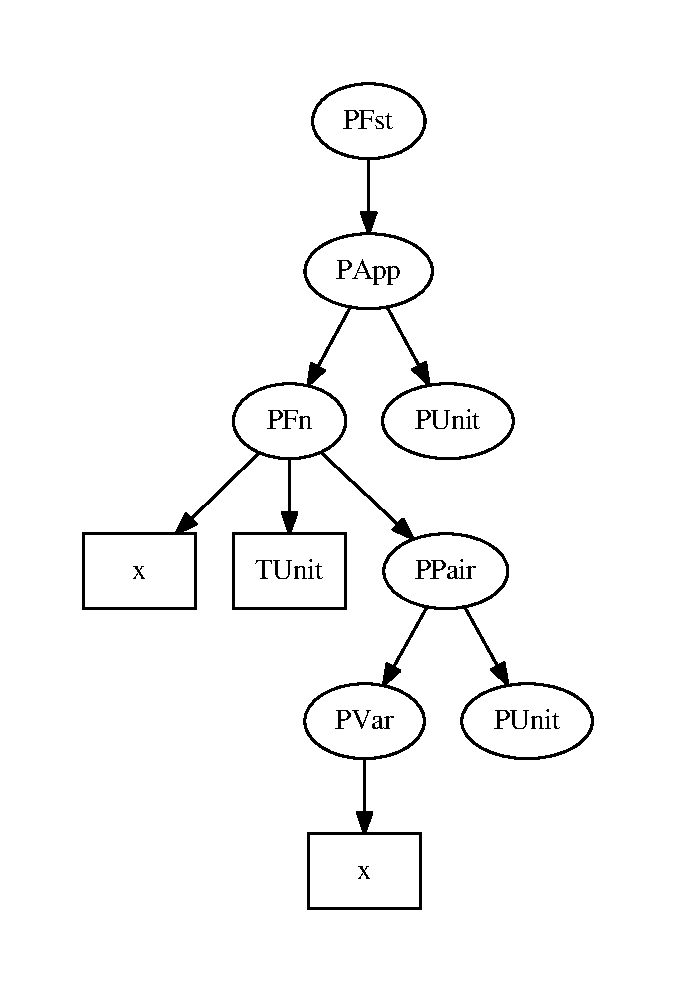
\includegraphics[height=4in]{chapters/evaluation/figures/example-tree.pdf}
\caption{an example syntax tree: syntactic nodes are shown by ellipses, with incidental data in boxes}
\label{fig:example-tree}
\end{figure}

\subsection{Experimental Method}
There is a problem in that asymptotic complexity cannot be determined by any performance measurements on finite inputs.
However, since type inference is only likely to be run on terms of a reasonable size, say, no more than \(10^5\), we can state that it has a certain complexity within a given range of sizes, then conjecture that this extends to an asymptotic result.

The experimental approach, is as follows:
\begin{enumerate}
\item
Generate representative test data of several different orders of magnitude in the reasonable range.
\item
Benchmark the algorithm on each of these test inputs and record performance.
\item
Correlate (logarithmic) runtime against (logarithmic) input size to determine an asymptotic performance bound.
A log/log plot is used since the range of values is too large to plot reasonably, but I do not wish to disturb the relationship between the data points.
Plotting both logarithmically allows us to display the relationship between inputs and runtime of several different orders of magnitude.
\end{enumerate}

Ideally the data generated would be (pseudo-) random, in order to prevent any patterns introduced in the test data from affecting the benchmark: the generators used to produce test data could then be repurposed to benchmark data.
Another constraint is that the expression must be well-typed in general, or the error propagating through will remove most of the processing from the benchmark.

Unfortunately, QuickCheck's random generation procedures turned out to be too slow to produce large randomised inputs efficiently.
QuickCheck uses the standard random package for generic applications which is not optimised for speed, and QuickCheck itself is not designed to produce large inputs, as its main use case is finding edge-cases (which tend to be smaller).
Benchmarking showed that random number generation was the bottleneck, but perhaps this would be different if QuickCheck were designed differently.
Instead, I used deterministic algorithms to produce large inputs, according to a variety of patterns:
\begin{enumerate}
\item well-typed terms, using all datatype constructors
\item pairs, with each sub-term a pair
\item projection functions applied to pairs repeatedly
\item applications, with each sub-term of equal size
\item applications, with unbalanced sub-terms
\item function binders in a chain
\item a sequence of binders, followed by bound variables
\end{enumerate}
These are designed to test general performance on varied inputs, on specific inputs, and finally to stress the typing context operations.
I then used the patterns to generate data, sized from 1, increasing by a factor of 10 to 100,000, and wrote the data to file for reproducibility (available under \texttt{infer/samples} in the source tree submitted with this dissertation).

Producing well-typed terms was quite tricky, even for this simple type system.
The general approach was for each generator to assume that any recursive calls generated well-typed terms, and maintain the invariant that the result it generates is also well-typed.
Then, the matter of choosing which sort of node was to be produced at any step in the recursive algorithm was done by taking the remainder of the size required and producing the corresponding type of data, which produced a well-distributed tree for a deterministic algorithm.
For instance, the algorithm for testing projections is shown in Figure \ref{figure:projection-sample}.

\begin{figure}
\begin{minted}{Haskell}
benchProjections :: Int -> Term
benchProjections n
  | (n <= 0) = PUnit
  | (n `mod` 2 == 0) = PSnd . PPair PUnit $ benchProjections (n - 2)
  | otherwise = PFst . flip PPair PUnit $ benchProjections (n - 2)
\end{minted}
\caption{The Haskell function generating a test of projection performance based on a size parameter.}
\label{figure:projection-sample}
\end{figure}

Benchmarking algorithms on small inputs (``micro-benchmarking'') has the problem of jitter: outside factors such as cache effects, branch prediction and kernel scheduling can all cause the same algorithm with the same input to run at different rates.

Haskell's laziness also adds another problem --- since the parameter passed to the function is not strictly-evaluated, the first evaluation of the function can take significantly longer as in this case the input needs to be loaded from disk and parsed before being processed.

Both these problems were solved by using the Criterion micro-benchmarking library~\cite{criterion}.
This solution deals with jitter by running the algorithm repeatedly and differing numbers of times to generate enough samples for a statistically significant result (generally an \(R^2\) value exceeding 0.99), and with laziness by evaluating the argument to a normal form first.

\subsection{Results}
Results were extremely positive for the \(O(|M|)\) hypothesis.
Figure \ref{fig:results-welltyped} shows a strong linear correlation for the general-performance dataset, while Figure \ref{fig:results-combined} supports this further, showing that every sort of structure produces linear performance on the target range.
The high levels of correlation on every graph lend extra credit to the hypothesis of a linear-time algorithm.
While it is possible that the algorithm is, in fact, super-linear (or sub-linear!), \emph{on the input range} the algorithm correlates well to a linear trend.

\begin{figure}
\centering
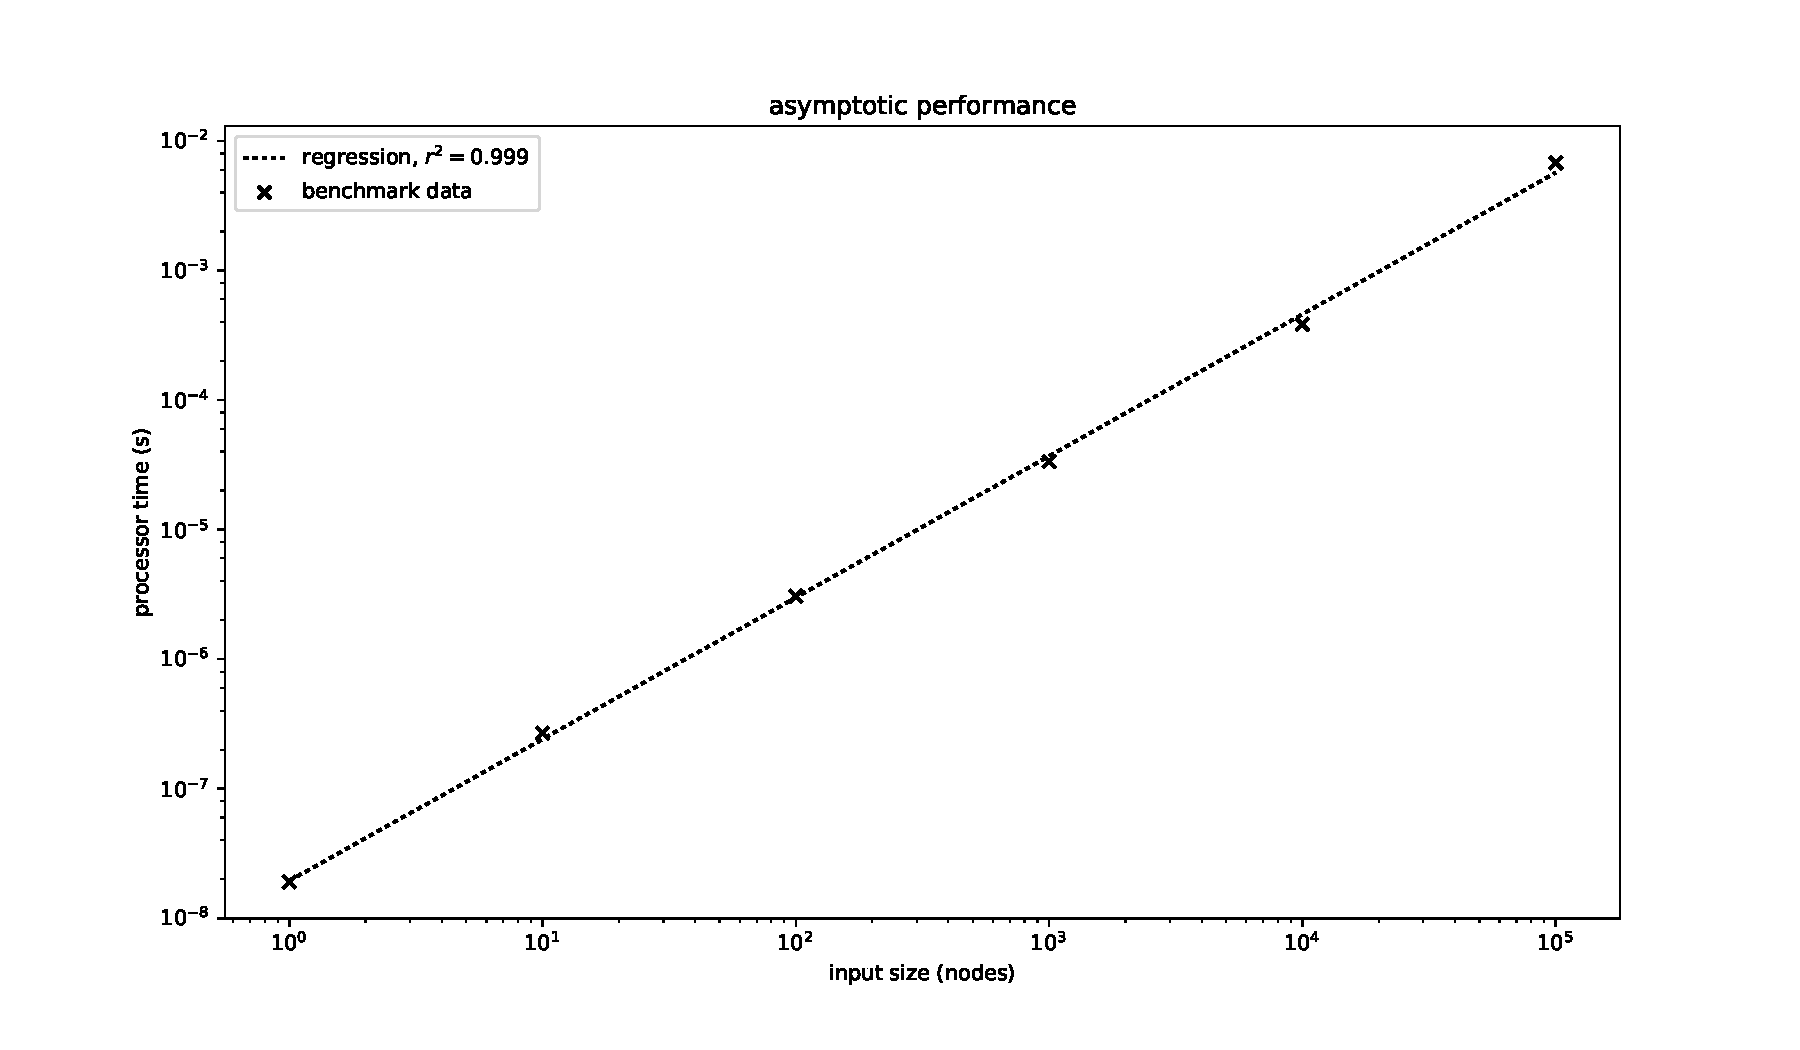
\includegraphics[width=\textwidth]{chapters/evaluation/plots/welltyped}
\caption{log-log plot of benchmark data size vs processor time, with a linear regression fitted}
\label{fig:results-welltyped}
\end{figure}

\begin{figure}
\centering
\begin{subfigure}{.49\textwidth}
 \centering
 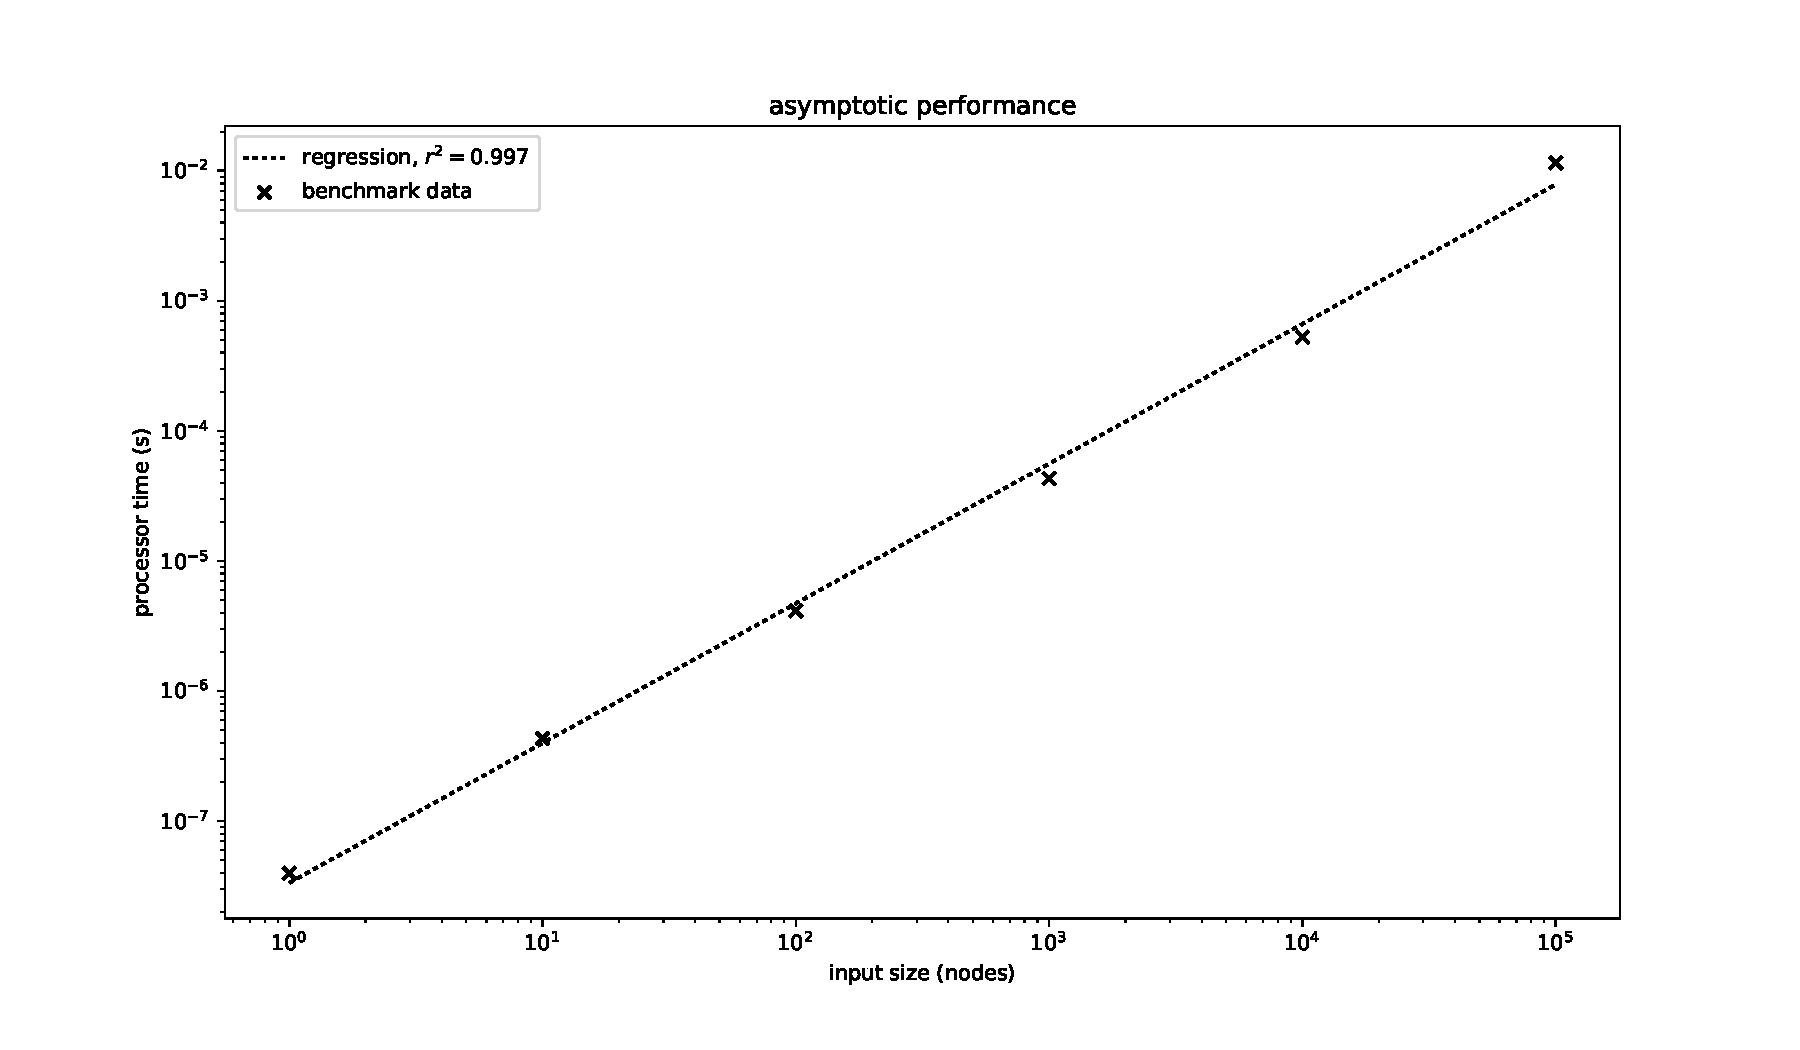
\includegraphics[width=\linewidth]{chapters/evaluation/plots/pair}
 \caption{pairs}
\end{subfigure}
\begin{subfigure}{.49\textwidth}
 \centering
 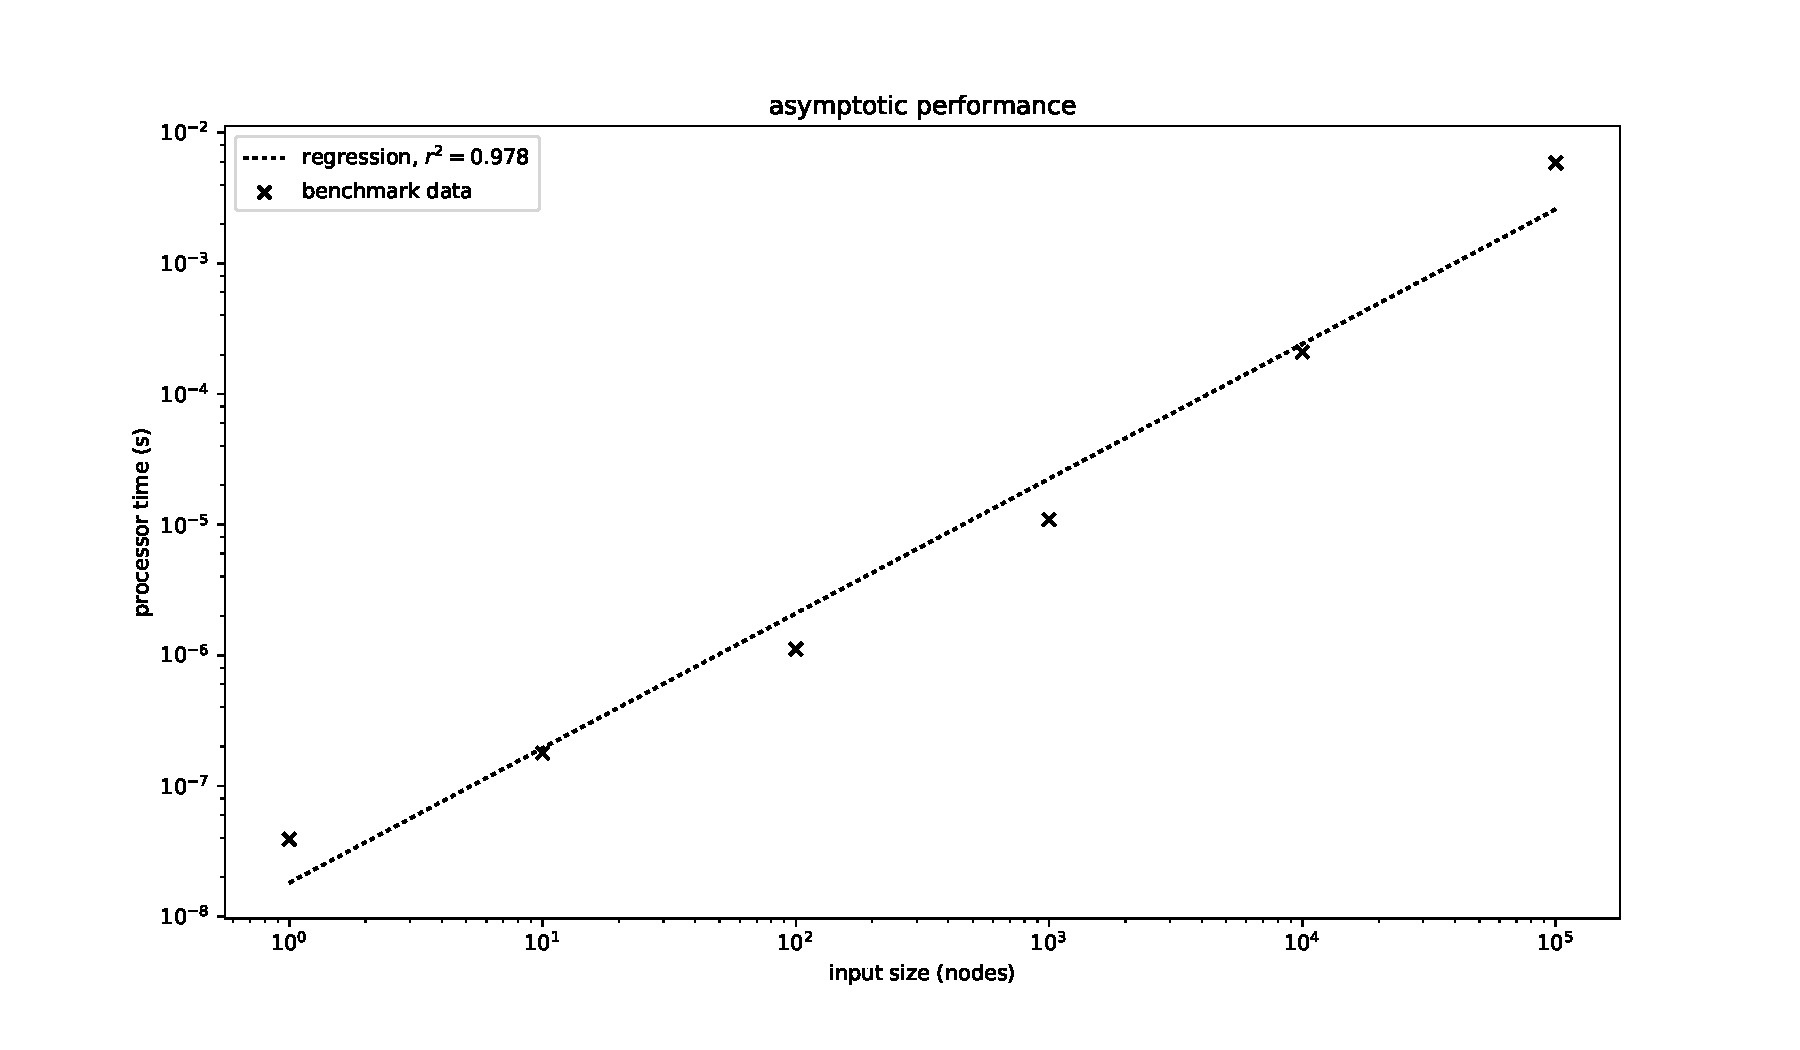
\includegraphics[width=\linewidth]{chapters/evaluation/plots/projections}
 \caption{projections}
\end{subfigure}
\begin{subfigure}{.49\textwidth}
 \centering
 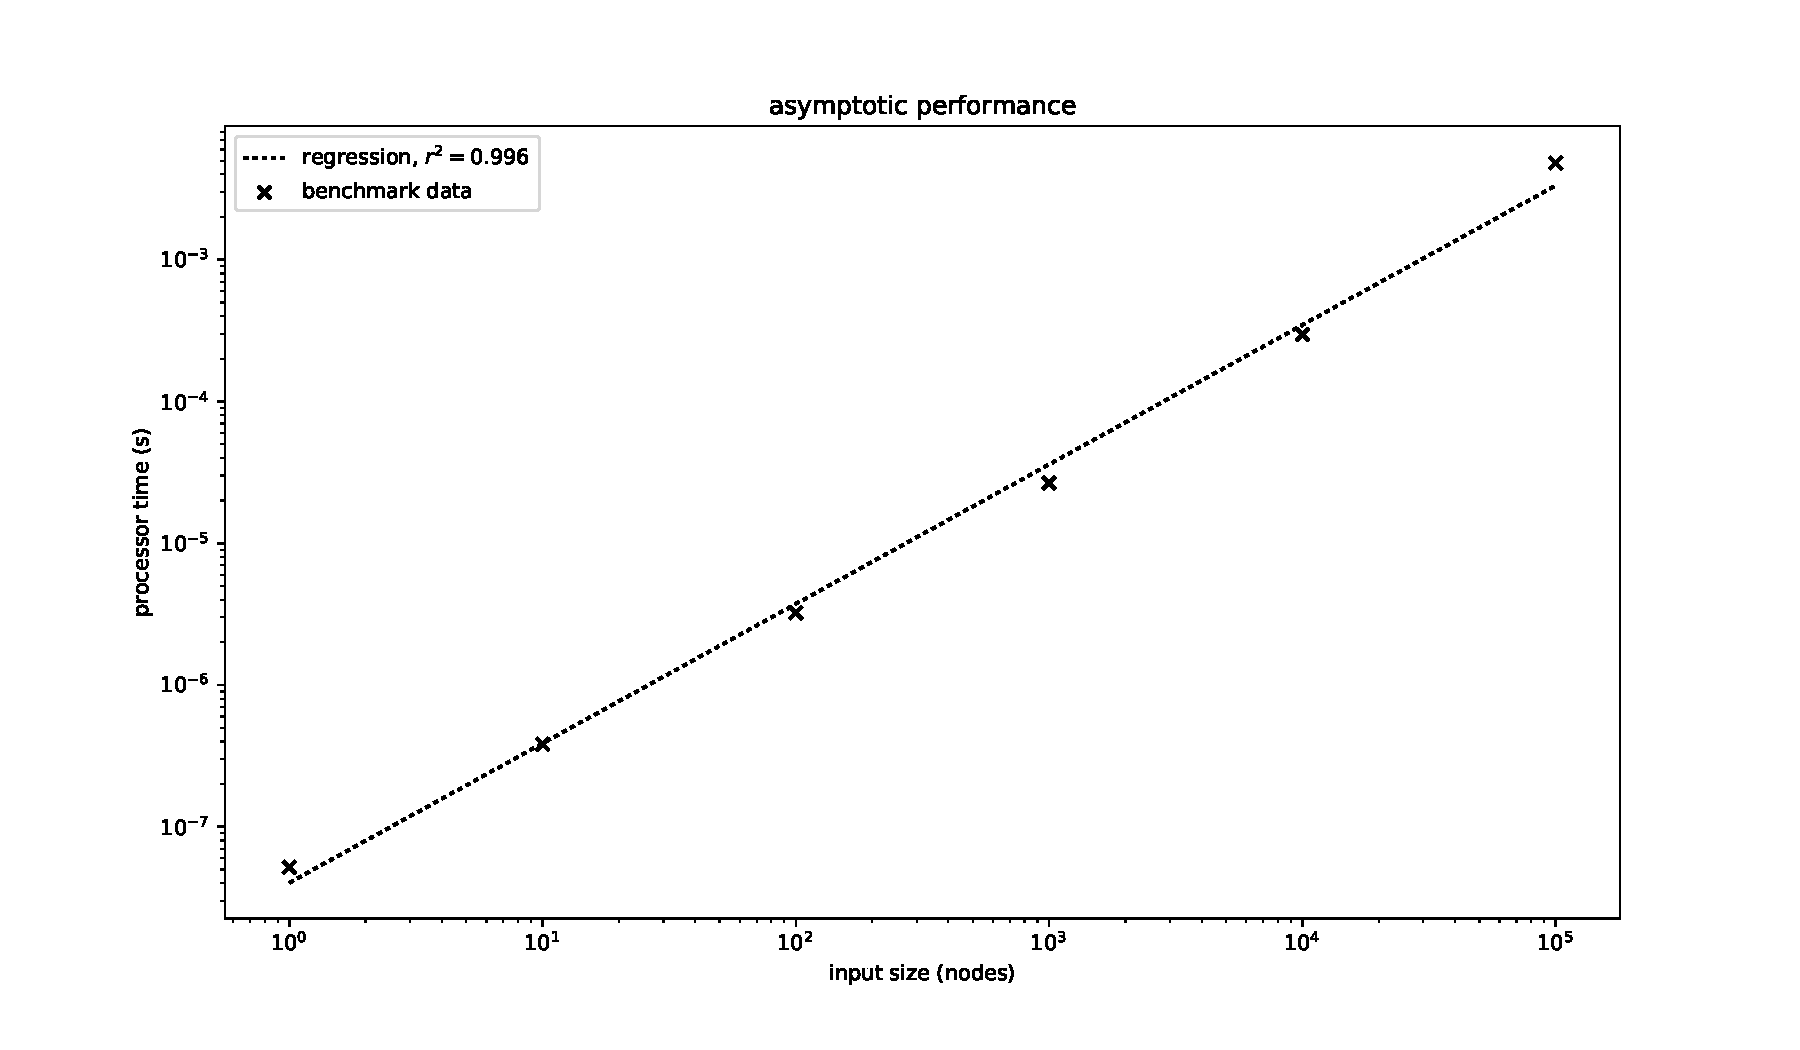
\includegraphics[width=\linewidth]{chapters/evaluation/plots/app}
 \caption{balanced applications}
\end{subfigure}
\begin{subfigure}{.49\textwidth}
 \centering
 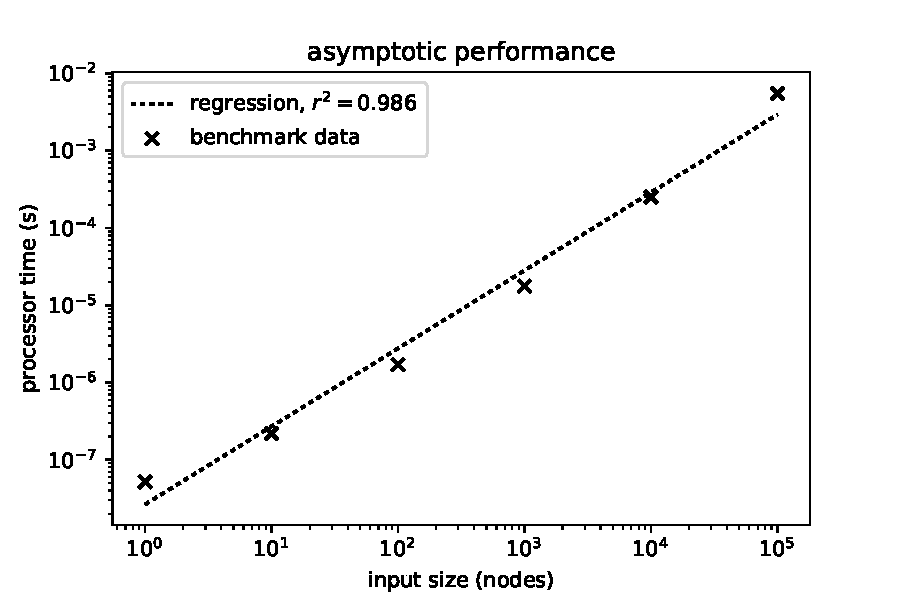
\includegraphics[width=\linewidth]{chapters/evaluation/plots/biased-app}
 \caption{applications, biased to one side}
\end{subfigure}
\begin{subfigure}{.49\textwidth}
 \centering
 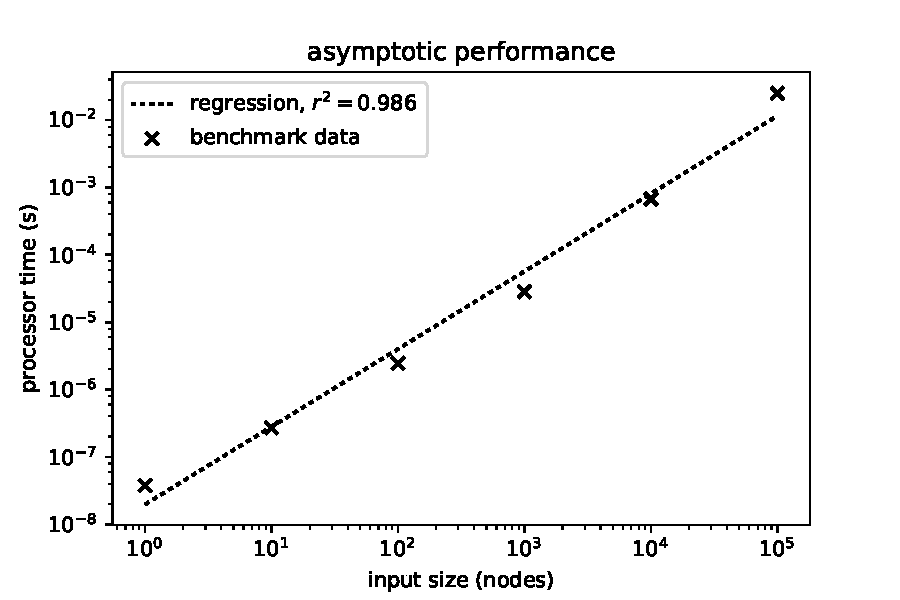
\includegraphics[width=\linewidth]{chapters/evaluation/plots/fn}
 \caption{chain of function binders}
\end{subfigure}
\begin{subfigure}{.49\textwidth}
 \centering
 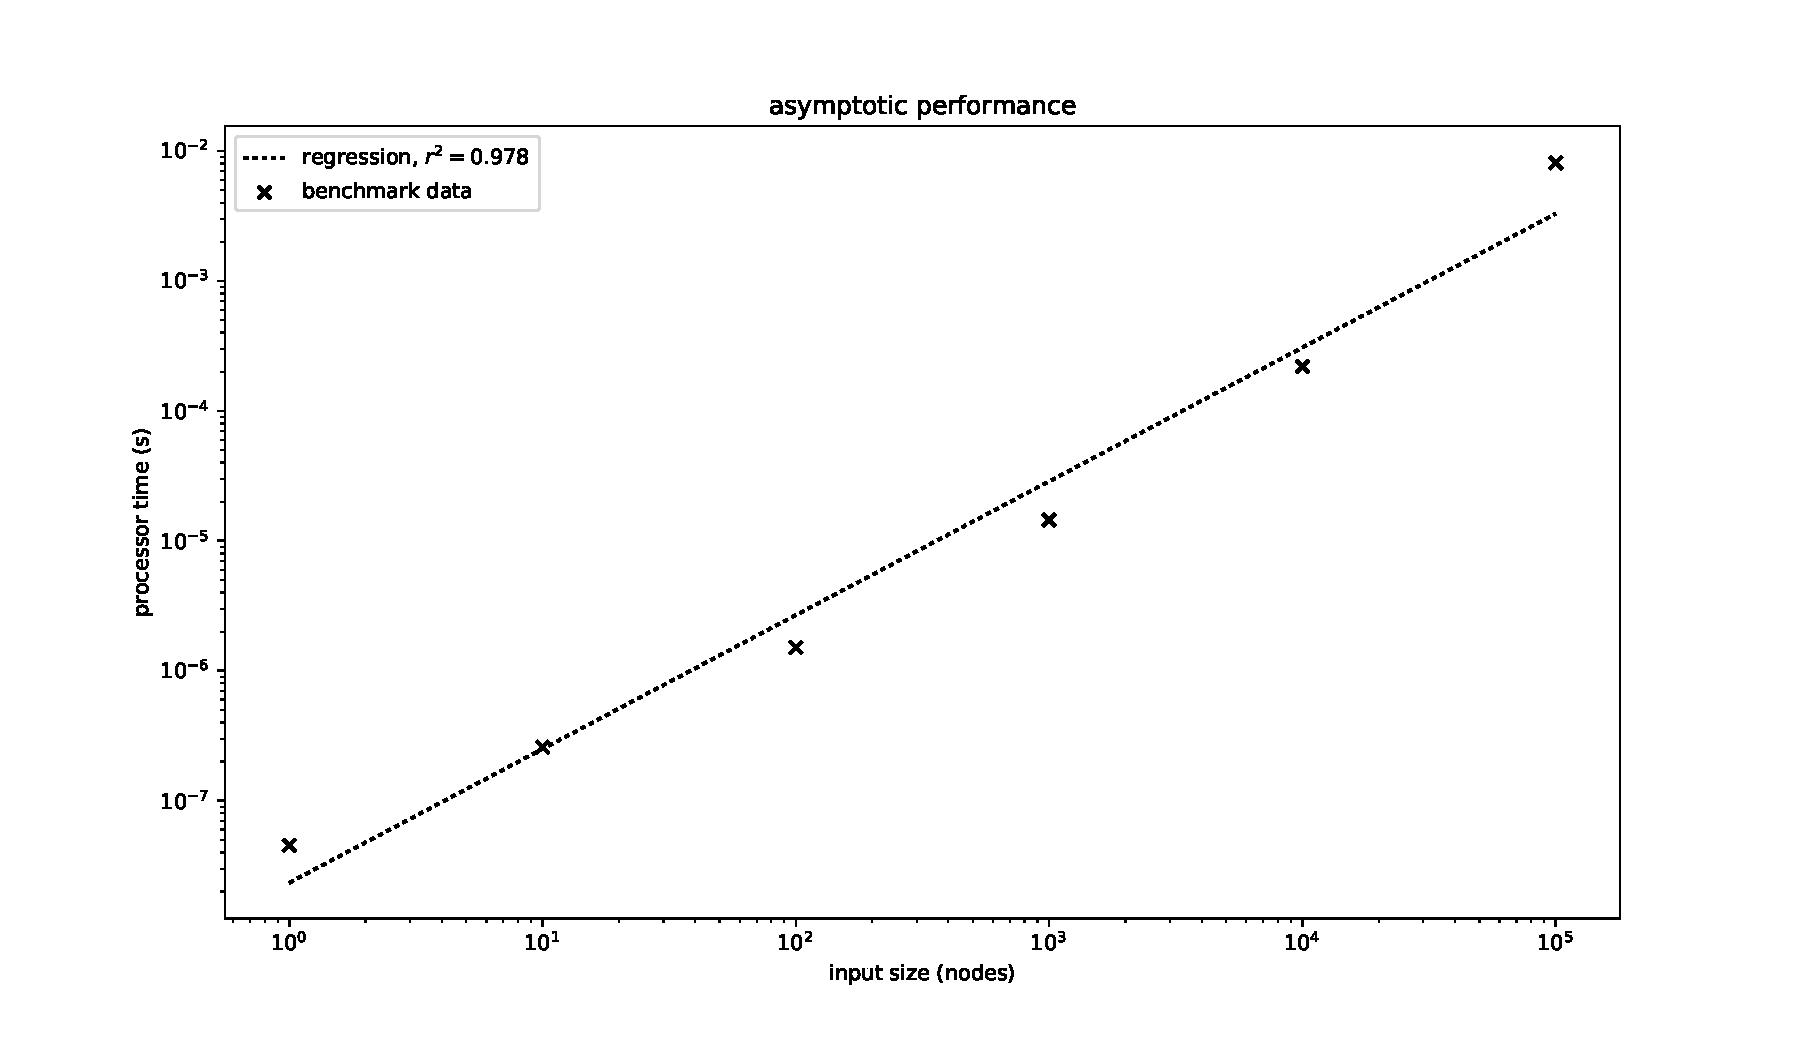
\includegraphics[width=\linewidth]{chapters/evaluation/plots/lookup}
 \caption{typing context stress}
\end{subfigure}
\caption{log-log plots (similar to Figure \ref{fig:results-welltyped}), showing performance on specialised inputs}
\label{fig:results-combined}
\end{figure}

Of particular interest is the context stress-test: this was included as the extracted code uses a method of representing finite maps using closures that should be extremely inefficient.
It implements the lookup and update operations as follows:

\begin{minted}{Haskell}
type Context k a = k -> Maybe a

lookup :: Context k a -> k -> Maybe a
lookup c k = c k

update :: Eq k => Context k a -> k -> a -> Context k a
update c k a = \x -> if x == k then Just a else c x

empty :: Context k a
empty = \x -> Nothing
\end{minted}

In the case of the extracted inference algorithm, this implementation of map should result in quadratic slowdown when applied to binders followed by variable lookup, as the closure representing the finite map grows in size.
Unexpectedly, in the typing-context dataset, this does not appear to be the case: even profiling the executable does not show significant time spent in the closure, or in the equality implementation.
It is possible that the compiler is able to spot the idiom of using a closure as a dictionary and optimise this away to a lookup table, or at least mitigate the poor performance of repeatedly branching to a new closure while looking up a key.
However, this seems very unlikely given the current level of optimisations possible.
GHC does use a somewhat unusual execution model~\cite{STG} as a compilation step, which may offer a performance improvement in this case, compared to the na\"ive idea of how such an algorithm is compiled to a physical architecture.
More likely is that the input size is simply not large enough yet to cause the linear-time lookup of the context to become significant compared to other (constant-time) parts of the algorithm.

However, I would still expect a reasonable implementation with e.g. an ordered map to be more performant: Figure \ref{fig:results-map} shows that a hand-implemented version using Haskell's \emph{containers} ordered-map implementation still matches a linear trend in the size of the input (as expected, since context lookup was not significant with the original implementation), but the implementation is considerably slower than the na\"ive version.
It seems that context lookup may well be inefficient, but on reasonable input sizes it does not take enough time to become significant.

\begin{figure}
\begin{subfigure}{.49\textwidth}
 \centering
 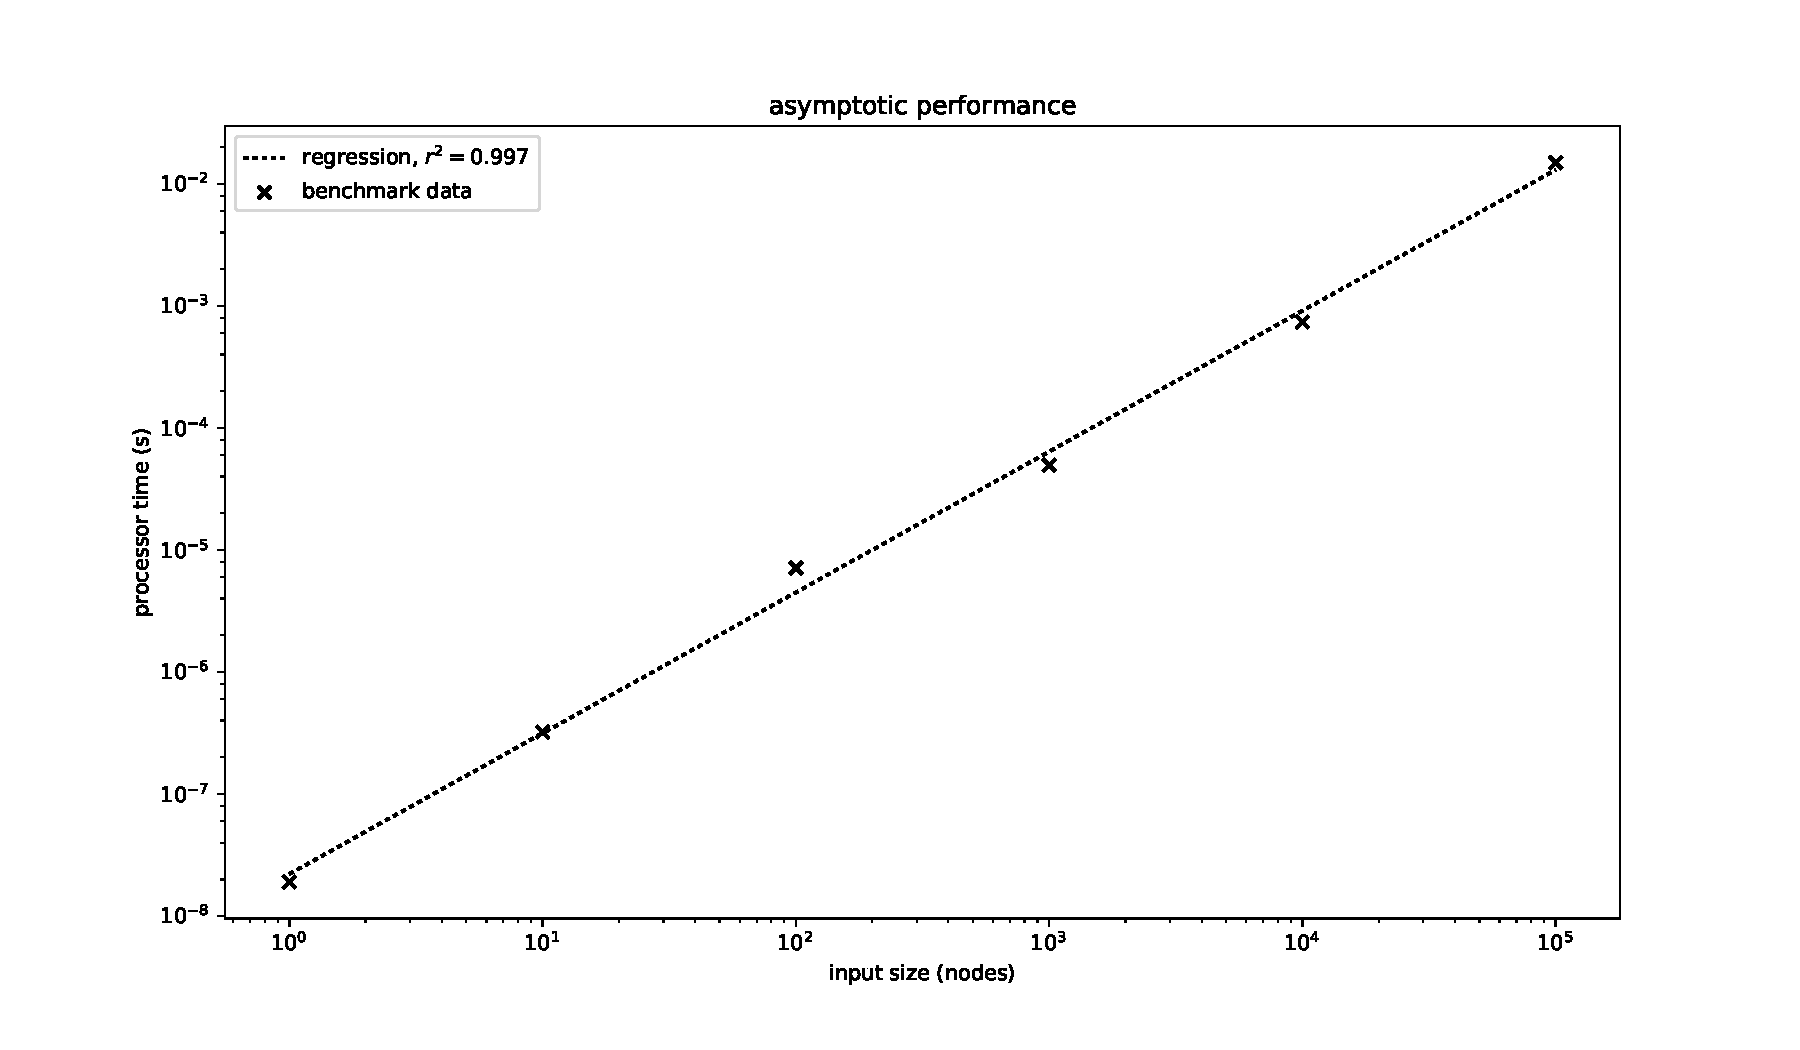
\includegraphics[width=\linewidth]{chapters/evaluation/plots/welltyped-map}
 \caption{asymptotic performance}
\end{subfigure}
\begin{subfigure}{.49\textwidth}
 \centering
 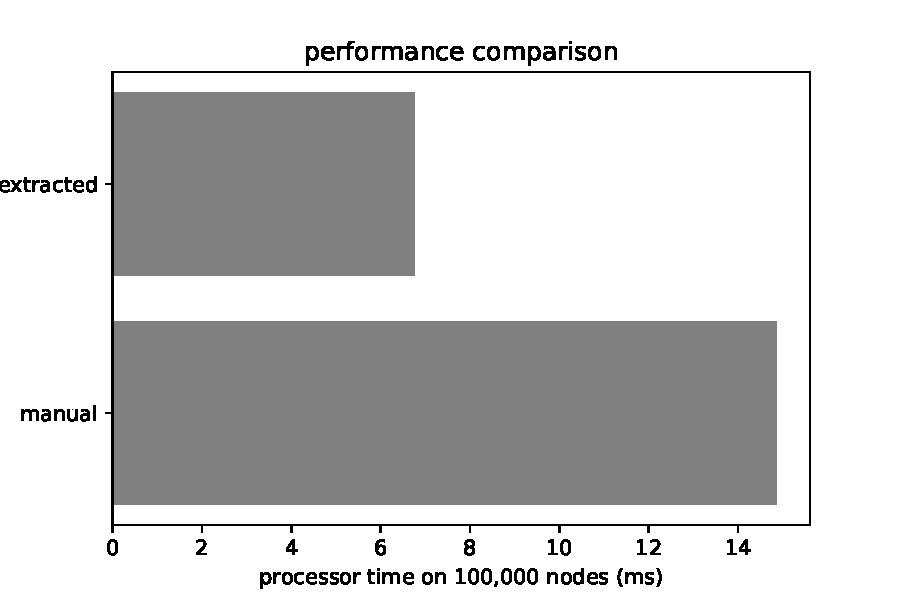
\includegraphics[width=\linewidth]{chapters/evaluation/plots/comparison}
 \caption{comparison against extracted code}
\end{subfigure}
\caption{plots showing the performance of the manual implementation}
\label{fig:results-map}
\end{figure}

\section{Comparison to Previous Work}
\label{sec:comparison}
There have been other Isabelle formalisations of typed \(\lambda\)-calculi.
Isabelle has its own implementation (in \texttt{src/HOL/Proofs/Lambda/} in the Isabelle source tree), which I will use as a context in which to evaluate my project --- using another implementation written with different proof tools would confuse the issue, as different tools produce different approaches to play to their strengths and weaknesses.

Despite using the same tooling, the two implementations are still very different: Isabelle's implementation uses chained, tactic-style reasoning almost exclusively, introduces types separately to terms, and uses a nameless representation of bound variables, whereas my project uses explicit reasoning steps almost exclusively, attaches an explicit type to every binder, and uses a named representation, combined with the use of a quotient type to represent \(\alpha\)-equivalence.

\subsection{Chained Tactics vs. Isar}
Using only tactics does tend to make the proof shorter (as can be seen from the proof lengths for comparable lemmas in both implementations: subject reduction is shown in approximately 15 lines in an apply-style proof, but my more explicitly-reasoned proof takes over 90), but can also (albeit subjectively) decrease readability of the generated proof~\cite{isar-phd}.
It should be noted that line count is not in general a good metric for proof length: the use of previous results and different proof approaches, proof steps, and tools can affect line count significantly.
Another advantage of the Isar approach is ease of learning: if I could not get a tactic to show what I wanted, it was easier to break down the proof statement into smaller steps using Isar and invoke a prover on each than it was to learn what sequence of tactic applications would produce the desired result.

\subsection{Church- vs. Curry-style Types}
The Isabelle implementation actually formalises the untyped calculus, before adding simple types afterwards.
This approach allows for multiple type systems to be implemented on top of a base that deals only with untyped operations, a great improvement on my project, which would need to be re-written totally in order to add a significant change to the type system.

However, not adding explicit types to binders does produce a marked difference in what the theory shows: this is now Curry-style typing, where the question for type schemes given a term \(M\) is no longer the Church-style ``what is the type of \(M\)?'', but ``what is the set of possible types for \(M\)?''.
Of course, this is intentional --- but if a Church-style typing system is desired, then this approach is not possible.

One way to achieve this modularity in a Church-style context would be to parameterise the datatype for representing terms over all possible datatypes for representing types, as well as variables.
With this modification, adding a new type system would involve only defining a new datatype representing the new types, and building the new typing system around the term parameterised by these new types.

Even more generally, most of the work with binders and substitution could be done on an abstract notion of terms-with-names.
Consider defining \emph{abstract terms} \(\mathcal A\) to be either
\begin{enumerate}
\item a variable (bound or free) \(x\)
\item a pair \((\mathcal A, \mathcal A)\)
\item a binder \(x_C.\mathcal A\), binding a variable in an abstract term with some ``context'' \(C\)
\end{enumerate}
This is sufficient to define \(\alpha\)-equivalence, substitution and so forth.
Then define a bijection \(f\) between abstract terms and the concrete terms of the simply-typed calculus as follows:
\begin{align*}
f(x) &= x\\
f((M\ N)) &= (f(M), f(N))\\
f(\lambda (x : C). M) &= x_C.f(M)
\end{align*}
and the obvious definition of \(f^{-1}\).
All reasoning purely about operations involving names can now be done on the abstract terms, then added to the concrete terms by defining the concrete operation in terms of the abstract operation and \(f\).

By way of example, suppose the notion of substitution on abstract terms has been defined, and that we have proven Barendregt's substitution lemma --- that is, if \(x \neq y\) and \(x\) is not free in \(\mathcal L\), then
\[
\mathcal M[x ::= \mathcal N][y ::= \mathcal L] = \mathcal M[y ::= \mathcal L][x ::= \mathcal N[y ::= \mathcal L]]
\]
It can now be shown without proving the lemma again that this property holds for the concrete terms as well.
Define substitution on concrete terms (using a different notation for clarity) by reference to substitution on abstract terms, using \(f\) as follows:
\[
M[N/x] \equiv f^{-1}\wrap{f(M)[x ::= f(N)]}
\]
Then the lemma holds easily, since
\begin{align*}
M[N/x][L/y]
	&\equiv \wrap{f^{-1}\wrap{f(M)[x ::= f(N)]}}[y ::= L]\\
	&\equiv f^{-1}\wrap{f\wrap{f^{-1}\wrap{f(M)[x ::= f(N)]}}[y ::= f(L)]}\\
	&\equiv f^{-1}\wrap{f(M)[x ::= f(N)][y ::= f(L)]}\\
	&\equiv f^{-1}\wrap{f(M)[y ::= f(L)][x ::= f(N)[y ::= f(L)]]}\\
	&\equiv f^{-1}\wrap{f\wrap{M[L/y]}[x ::= f(N)[y ::= f(L)]]}\\
	&\equiv f^{-1}\wrap{f\wrap{M[L/y]}[x ::= f\wrap{N[L/y]}]}\\
	&\equiv M[L/y][N[L/y]/x]
\end{align*}

These terms also form a nominal set with similar structure to the original calculus, so all results still hold with little modification.
In this way a level of modularity and re-usability can be achieved, without sacrificing Church-style typing.
Currently, the amount of project-specific Isabelle stands at around 4000 lines, with around 500 lines of reusable theories.
With this modification, the majority of work would be re-usable, and the only project-specific work to deal with names would be defining a bijection with these abstract terms and any language with similar semantics about binders.
While this idea is my own, it was previously found in a more general form by Gabbay \emph{et al}~\cite{nominal-algebra}.
Implementing this approach as a library in Isabelle is left as future work.

\subsection{Approaches to Binders}
The treatment of binders is a difficult part of the formalisation of any system that uses them.
The authors of the \textsc{PoplMark} challenge~\cite{poplmark} specifically mention this topic, and note that, of the solutions they have seen, there was no clear winner.

It can be seen from the extremely-small Isabelle implementation of de Bruijn indices that a nameless representation (where \(\alpha\)-equivalence is simply equality) is much easier to formalise initially than the approach taken in my project --- no permutation lemmas, no \(\alpha\)-equivalence arguments, no quotient types and so on.
However, the subsequent effort required to argue simple theorems such as the substitution lemma described above with de Bruijn indices is significant.
Berghofer and Urban argue~\cite{head-to-head} that a nominal representation has many advantages over indices, particularly in the context of the \textsc{PoplMark} challenge, once the initial infrastructure has been set up.
They mention that de Bruijn indices are convenient to define, but become tedious after a while (at least in the context of \textsc{PoplMark}), while nominal techniques have a significant setup cost but are convenient thereafter in general.
However, the paper does not draw a significant conclusion as the scope of usage is limited to only a few problems.

Assuming that Berghofer and Urban's conclusions and my own are correct, then, nameless representations are a good choice for (shorter) implementations that do not use the binding aspects of \(\lambda\)-calculus much, whereas the initial effort of nominal methods produce easier results when applied to more difficult theorems about binding.
Additionally, the named representation is arguably more human-readable and presents less notational impedance than the nameless version, promoting later re-use.

\subsection{Nominal Implementation}
An important comparison to draw is that of a manual approach to a nominal implementation, with that of Nominal Isabelle.
I chose to perform things manually, as neither Nominal Isabelle, nor its successor Nominal 2 support code generation at the time of writing, and code generation was a required part of the project.

Unfortunately, this led to a lot of effort, that while educational, could have been avoided with use of the automation provided by Nominal Isabelle.
I had to manually implement:
\begin{itemize}
\item
A theory of permutations.
While a theory was added to Isabelle's library after I began my project, initially there was no implementation of permutations in the standard library.
\item
(strong) Induction principles for \(\alpha\)-equivalent terms.
\item
A quotient type.
\item
Inequality rules for these terms, such as \(\forall A, B.\ (A, B) \neq \unit\) --- these are particularly unfortunate as the number of lemmas required grow quadratically with the number of different varieties of term.
\item
Structural equality rules, such as \(\forall A, B.\wrap{\pi_1(A) = \pi_1(B) \implies A = B}\).
\item
Proofs showing that functions on pre-quotient terms can also be functions on \(\alpha\)-equivalence classes, like the type inference function, then lifting them over the quotient.
This property is not true in general (consider the function that returns the bound variables of a term), but Nominal Isabelle provides a couple of ways to define functions which generate a proof obligation to show this property~\cite{fresh-fun}.
\end{itemize}

Nominal Isabelle would have saved a considerable amount of effort, and made several tedious aspects of the project significantly shorter.
However, the ability to extract code allowed the project to be more practically useful, and testing this allowed for another dimension that would not have been avaible with Nominal Isabelle.

\section{Lessons Learned}
\label{sec:lessons}
I learned several lessons during the course of the project.
The first and most important, was that the treatment of names in any language featuring binders is a large aspect of formalising the language.
Considerable thought must be dedicated to correctly-formalising the precise semantics of an area that is traditionally avoided as mathematically uninteresting.

Secondly, there is a tradeoff between preparatory work and ease of use: nameless representations of the \(\lambda\)-calculus allow for an easy definition of both the calculus and \(\alpha\)-equivalence, but become tedious to use later on.
Nominal techniques require a lot of initial work to set up, but make subsequent work easier by comparison to nameless representations.

More practically, extracting code from formalised implementations produces correct code, but it may have unusual performance characteristics that do not match the idealised versions.

\section{Summary}
In this chapter, I prepared the project for evaluation (\S\ref{sec:framework}), ran some property tests to add confidence of the project's correctness (\S\ref{sec:property-testing}).
Moving on to benchmarking, I produced some benchmark data, then ran benchmarks to determine both asymptotic and relative performance of the inference algorithm (\S\ref{sec:benchmarking}).
Finally, I evaluated techniques for implementing this project's brief against similar work (comparing proof styles, church and curry-style typing, approaches to binders, and automatic versus manual nominal implementation) in Isabelle (\S\ref{sec:comparison}), before finishing with the lessons I learned from the project (\S\ref{sec:lessons}).

\chapter{Conclusion}
I have shown the development of a formalised implementation of a typed \(\lambda\)-calculus in the proof assistant Isabelle, complete with correctness properties about the type system and verified, extracted, code for type inference.
All success criteria have been met, and some extensions have been made, augmenting the core calculus and showing the confluence property.
This work differs from, and improves upon a typical implementation in its use of nominal techniques that have several advantages over other methods of name binding.

\section{List of Results}
Taking success criteria from my project proposal, they have all been met:
\begin{enumerate}
\item
I have now learned sufficient theory to understand, implement, and justify my approach to the problem.
\item
I gained sufficient practical experience before and during my project about the Isabelle proof assistant to efficiently implement the project.
\item
The representation of the calculus I chose has been sufficient to produce the rest of my dissertation with.
\item
I have proven the progress, preservation, and safety properties of the type system.
\item
The implementation of type inference has been verified by showing it equivalent to the inductive typing rules.
\item
The extracted Standard ML code does compile and run as expected.
Although Haskell was the language I eventually used for testing, I don't consider that this change of decision disqualifies this success criterion.
\item
The dissertation is complete.
\end{enumerate}

\section{Further Work}
There is significant scope for further work in this area, and any one of several areas could be pursued.
Improving the nominal approach is one possible extension, perhaps adding some automation to remove some of the painful points.
Perhaps Nominal Isabelle could be improved/extended so that code extraction is possible, or alternatively the abstract-term approach could be implemented so that only relevant theory is implemented for any given system and issues of names can be avoided altogether.

Alternatively, extending or modifying the calculus to more interesting calculi, like System F.
System F includes binders at the type level as well as at the term level, so this would be a good test of the nominal approach when multiple binders are present.
Additionally, the type system is much more complex, allowing for more practical programming, while (with some restrictions) type inference remains decidable~\cite{hindley-milner}.

Improving performance of the extracted code is certainly possible.
While performance of the extracted code (surprisingly) is good without modification, I do not yet know \emph{why} this is the case.
Investigating this will no doubt lead to some optimisations.
Combined with a more powerful type system (such as System F), there are plenty of opportunities for efficiency improvements.

Further properties of the calculus can be shown, such as the strong normalisation property.
Strong normalisation is an important property of the simply-typed calculus from the perspective of computability theory, as it shows that the calculus is not Turing-complete (Turing machines may run forever).

\section{Closing Remarks}
\(\lambda\)-calculus produces a model of computation by manipulating terms involving bound and unbound names.
By investigating a variety of approaches to binding names, and implementing the most theoretically-pleasing approach, I have arrived at a verified representation of the \(\lambda\)-calculus, as used informally in mathematical arguments.
Further, I have shown that representing \(\lambda\)-terms by means of an explicit quotient with a nominal equivalence relation over the concrete syntax is laborious, but feasible as an approach, and comes with many advantages.

\addcontentsline{toc}{chapter}{Bibliography}
\printbibliography
\appendix
\chapter{Project Proposal}
\documentclass[12pt]{article}
\title{Part II Project Proposal: Formalising Simply-Typed \(\lambda\)-Calculus}
\author{Michael Rawson}

\usepackage[backend=bibtex,sorting=none]{biblatex}
\bibliography{proposal}
\begin{document}
\begin{titlepage}
%\thispagestyle{empty}

\rightline{\large Michael Rawson}
\medskip
\rightline{\large Robinson College}
\medskip
\rightline{\large mr644}

\vfil

\centerline{\large Part II Project Proposal, Computer Science Tripos}
\vspace{0.4in}
\centerline{\Large\bf Verified Metatheory and Type Inference}
\centerline{\Large\bf for a Name-Carrying Simply-Typed \(\lambda\)-Calculus}
\vspace{0.3in}
\centerline{\large \today}

\vfil

{\bf Project Originator:} Dr.~Dominic Mulligan

\vspace{0.1in}

{\bf Resources Required:} None

\vspace{0.5in}

{\bf Project Supervisor:} Dr.~Dominic Mulligan

\vspace{0.2in}

{\bf Signature:}

\vspace{0.5in}

{\bf Director of Studies:} Dr.~Alastair Beresford

\vspace{0.2in}

{\bf Signature:}

\vspace{0.5in}

{\bf Overseers:} Dr.~Ian Wassell and Prof.~Lawrence Paulson

\vspace{0.2in}

{\bf Signatures:}

\vfil
\end{titlepage}


\section*{Introduction}
\(\lambda\)-calculus (see \parencite{lambda-overview} for an overview) is a formal system of terms, often used in computability theory, but also more recently as a base system for various \emph{type theories}.

The calculus expresses computation as a series of \emph{abstractions} (anonymous first-class functions) and \emph{applications} (function application), with reduction relations between them.
For example, the identity function
\[
\lambda x.x
\]
applied to some term, say \(T\), is clearly \(T\): thus, the term
\[
(\lambda x.x)\ T
\]
reduces to \(T\).

This calculus, the ``untyped'' \(\lambda\)-calculus, clearly lacks any sort of type system.
Adding types to the calculus allows for various \emph{typed} \(\lambda\)-calculi: these add many useful properties, including strong normalisation for some calculi\parencite{strong-normalisation}, even allowing for mathematical theorems to be expressed under the ``propositions-as-types'' slogan\parencite{curry-howard}.
The simplest of these is the \emph{simply-typed} calculus \(\lambda_\to\), consisting only of type names \(A, B, \ldots\) and a function-arrow type constructor, e.g. \(A \to B\).

\emph{Formalising} such a calculus in a computerised proof assistant has several advantages: for one thing, theorems and proofs about the calculus can be expressed, and therefore automated, in the assistant.
For another, it allows the generation of formally-verified code from the assistant to a target language more suited for execution, thus achieving the holy grail of bug-free software development.

Therefore, I propose that I use Isabelle, a mature and versatile proof assistant \parencite{isabelle-overview} to formalise \(\lambda_\to\) and prove some metatheory about the encoded calculus.
In order to achieve this, and by means of innovation, I will also attempt to use an unusual method for encoding the calculus' bound variables.
Finally, to better evaluate my work, I will implement a type inference algorithm for \(\lambda_\to\), prove it correct, then extract executable code for it.

\section*{Required Resources}
No extra resources other than the Isabelle software package is required for this project.
Isabelle's 2016 release is freely available online\parencite{isabelle-installation}, so this should not present a problem.

\section*{Starting Point}
I'm familiar with types and the \(\lambda\)-calculus, both together and separately, through extra-curricular study and through the various theory courses present in part I of the tripos.

However, I'm not familiar with the Isabelle proof assistant, or with any similar proof assistants with a structured proof language, or with the underlying logical system (in Isabelle's case, this is in fact interchangeable, but I'll be using the default option, \emph{Isabelle/HOL}).
I have been given a crash course in the assistant by my supervisor over the course of the summer break in the form of exercises, reading, and advice, but my Isabelle could still use some improvement.

\section*{Structure of the Project}
The aim of this project is to verify some metatheory about the calculus, but I will use the goal of producing a verified type inference implementation to drive this process.
Additionally, this type inference goal allows me to evaluate the project more intelligently than as a collection of theorems.
A number of design choices have already been made in order to make a concrete plan.
\begin{enumerate}
\item
The \(\lambda\)-calculus contains \emph{binding} terms, the abstractions, which it uses to bind variables ``under'' the term.
The subject of binders is surprisingly complex, with many possible representations, including:
\begin{itemize}
\item
a concrete representation involving explicitly-bound variables
\item
de Bruijn indices, in which variables are referred to by the number of binders from the point of reference
\item
higher-order abstract syntax, which embeds the binding in the implementation language's binders
\item
more complex approaches involving \emph{permutations} of variables, such as in Nominal Logic\parencite{binding}
\end{itemize}
I have chosen the permutation approach, as it is the most mathematically interesting and offers some advantages over other approaches (as argued in \parencite{binding}).
A further advantage of this explicit approach to name-carrying over existing implementations, such as Nominal Isabelle, is the ability to extract executable code from the verification.

\item
In a similar vein, the notion of \(\alpha\)-equivalence --- that is, two terms are equivalent iff they are the same except for their use of different bound variable names: \(f(x) = x^2\) and \(f(y) = y^2\) would be said to be \(\alpha\)-equivalent --- needs to be expressed in the statement of lemmas in order to be fully general.
This can either be interjected wherever necessary, or equality of terms can be redefined using Isabelle's \emph{quotient type} implementation.
The latter simplifies later lemma definitions in exchange for implementation difficulty, so I have chosen the quotient-type option for greater elegance.
\item
The simply-typed calculus is often extended to allow general recursion by means of a fixpoint operator.
I've chosen not to implement this, as it significantly complicates the theory by allowing \(\lambda_\to\) to become Turing-powerful.
\item
Several properties of the implementation can be used to check its correctness.
Specifically, I will prove the progress, type-preservation, and safety properties (as seen in the part IB semantics course) for my implementation.
Additionally, I will show that the type-checking procedure always produces the same results as the type inference rules expressed inductively.
This should suffice to ``verify'' the implementation has been formalised as expected.
\end{enumerate}

The structure of the project is as follows, with several main sections:
\begin{enumerate}
\item
An in-depth study of the simply-typed calculus and varieties (see above), to ensure I have details correct before starting work.
\item
Any necessary research in order to operate the Isabelle package effectively for this task.
\item
Development of the representation and operations of the calculus in Isabelle, allowing expression of more complex theorems.
\item
Proof of the progress, preservation, and safety properties of the calculus, following on from the representational work.
\item
Implementing and verifying the type inference algorithm.
\item
Extracting Standard ML code for the algorithm.
\item
Producing the dissertation.
\end{enumerate}

\section*{Success Criteria}
Each section from the project has its own success criterion:
\begin{enumerate}
\item
Do I have sufficient \emph{theoretical} knowledge to implement the project confidently?
\item
Do I have sufficient \emph{practical} knowledge to implement the project confidently?
\item
Can I verify the representation is correct with later proofs?
\item
Have I proven the aforementioned properties for the encoded calculus?
\item
Is the type inference algorithm verifiable?
\item
Does the Standard ML code compile/work as expected?
\item
Is the dissertation complete?
\end{enumerate}
Since the project is formally-verified, the final success criterion is remarkably simple: does the proof assistant tell me that I have proved my theorems?

In order to properly evaluate the project, some other metrics of success might be employed:
\begin{itemize}
\item
speed of generated code
\item
fuzz-testing generated code, as a sanity check
\item
quality/complexity of the formalisation: compare my implementation to prior art for code quality or complexity
\item
compare and contrast my unusual approach of using Isabelle's quotient types directly for name binding with other approaches
\end{itemize}

In case of finishing early, I have also planned some extensions:
\begin{itemize}
\item
extend the implementation to more advanced calculi, like System F or \(\lambda\Pi\)
\item
prove more properties about the calculus, like the congruence property --- almost any metatheoretical result about the calculus is relevant here
\item
experiment with different formulations of the type inference algorithm and observe the effects on generated code and its performance
\end{itemize}
\section*{Timetable}
In 10 fortnightly steps, the proposed timetable for this project is as follows:
\begin{enumerate}
\item
Prepatory academic work: survey the current state of the art, particularly in the areas of name-binding and typed calculi.
I should be able to implement and explain ideas from relevant papers in order to complete my project.
\item
Prepatory practical work: experiment and practise with the Isabelle proof assistant.
I should be able to express relevant ideas and theorems more easily in the software.
\item
Encode the calculus in Isabelle and start work on the permutation approach to \(\alpha\)-equivalence.
\item
Finish work on the permutation theory and encode equivalence with a quotient type.
I will already have proven some vital properties of the calculus at this point to show that equivalence of terms is an equivalence relation.
\item
Start proving properties about the calculus.
I will aim to finish at least a few to show for the progress report and presentation.
\item
Complete as many properties as possible before moving on to the type inference.
Implement the type inference algorithm and extract executable code for it.
\item
Verify the type inference algorithm behaves correctly and finish any remaining tasks for the practical work.
\item
Start writing the dissertation.
The Introduction and Preparation chapters should be complete, with the Implementation chapter started.
\item
Finish writing the dissertation.
All chapters should be complete as far as possible at this point.
\item
Review, proof-read and make any required changes to the dissertation.
Reserve space for submission and emergencies.
\end{enumerate}
\printbibliography
\end{document}

\end{document}
